\documentclass[a4paper,12pt]{article}
\usepackage[utf8x]{inputenc}
\usepackage[T1]{fontenc}

%\usepackage[T2A]{fontenc} % jei yra kirilica
\usepackage[hmargin={30mm,15mm},vmargin={20mm,20mm},bindingoffset=0mm]{geometry}
\usepackage[onehalfspacing]{setspace}
\usepackage[colorlinks=true, linkcolor=blue, citecolor=blue, urlcolor=blue, unicode]{hyperref}

%\parindent=7mm
\renewcommand{\refname}{Literatūros sąrašas} % article
%\renewcommand{\bibname}{Literatūros sąrašas} % report
\renewcommand{\contentsname}{Turinys}
\usepackage[T1]{fontenc} 

% Lukas paketai
\usepackage{lmodern,textcomp}
\usepackage{booktabs}% http://ctan.org/pkg/booktabs
\newcommand{\tabitem}{~~\llap{\textbullet}~~}
\usepackage{graphicx}
\usepackage{verbatim}
\usepackage{indentfirst}
\usepackage{setspace}
\usepackage{placeins}
\usepackage{booktabs}% http://ctan.org/pkg/booktabs
\usepackage{tabularx}% http://ctan.org/pkg/tabularx
\usepackage[parfill]{parskip}
\usepackage[unicode]{hyperref}
\usepackage{hyperref}
\usepackage{tocloft}
\usepackage{graphicx}
\newcommand\AtPageUpperRight[1]{\AtPageUpperLeft{%
   \makebox[\paperwidth][r]{#1}}}
\usepackage[dotinlabels]{titletoc}
\usepackage[capposition=top]{floatrow}
\hypersetup{
    colorlinks,
    citecolor=black,
    filecolor=black,
    linkcolor=black,
    urlcolor=black
}
\usepackage{secdot}




\begin{document}
\graphicspath{ {/} }

\renewcommand{\cftdot}{.}	
\renewcommand{\cftsecleader}{\cftdotfill{\cftdotsep}}

\thispagestyle{empty} % nerasomas psl. nr


\begin{center}
 VILNIAUS UNIVERSITETAS 
 
MATEMATIKOS IR INFORMATIKOS FAKULTETAS

MATEMATINĖS INFORMATIKOS KATEDRA

\vspace{4cm}

Projekto vadovas \ \ \textbf{Lukas Tutkus} \\
\textbf{Julius Daukšas} \\
\textbf{Dominykas Smaliukas} \\
\textbf{Robert Stankevič} \\

\vspace{0.2cm}

Bioinformatikos studijų programos grupė BioSawmill



\vspace{3cm}
\textbf{\Large Programų sistemos projektas}\\


\vfill

Vilnius \ \  2015
\end{center}



\clearpage

\tableofcontents
\clearpage

\section{Duomenų bazės struktūra}


\section{Sistemos architektūra}


\section{Sudėtingesnių modulių veikimo apibrėžimai}

\subsection{ Paskyros parametrų keitimas }

\subsubsection{Parametrų keitimas}
Prisijungus galima pakeisti norimus paskyros duomenis.\\
Vartotojas gali keisti savo paskyros duomenis: \\
	prisijungimo vardą, el. paštą, slaptažodį. \\\\
	
Administratoriui atidariui paskyros keitimo langą\\
atsiranda sąrašas vartotojų. Spaudžiamas vartotojo \\
keitimo mygtukas "keisti" atsiradęs paspaudus ant vartotojo.\\
Dėl duomenų saugumo administratorius gali pakeisti tik\\
vartotojų prisijungimo vardus ir prisijungimo paštus. \\\\

Pakeitimai turi atitikti registracijos formos reikalavimus: \\
	\tabitem prisijungimo vardas >= 4 simboliai\\
	\tabitem unikalus paštas bei prisijungimo vardas.
    \tabitem slaptažodis >= 8 simboliai. \\\\
    
Pakeitimai patikrinami ir jei nera klaidų tada užklausa siunčiama \\
į duomenų bazėje. Taip pat pakeisti duomenys atnaujinami administratoriaus \\
vartotojų paskyrų sąraše. \\
Jei klaidų randama - neatitinka reikalavimų tada pažymimi neleistinas \\
reikšmes įgiję laukai.\\

\subsubsection{P.O. mokestis}
P.O. mokėjimą galima atlikti po prisijungimo. \\
Vartotojas paspaudęs mokėjimo mygtuką nurodo:
\begin{itemize}
	\item Aktyvuojamo vartotojo pašto adresą.
	\item Mokėjimo laikotarpį.
	\item Datą laikotarpio pradžiai.
\end{itemize} 
Mokėjimo laikotarpiai yra mėnesis(5€) ir metai(25€). \\
Jei vartotojas-aktyvuotas prie laikotarpio nurodoma galiojimo laikas.\\
Tokiu atveju vartotojas gali tik pratesti pagal pasirinktą laikotarpį 
bei data vėlesne už paskutinę galiojimo dieną.\\
Jei vartotojas-neaktyvuotas tada nurodo mokėjimo laikotarpį bei datą,
ne ankstesnę už šiandienos datą. \\
Spaudžiamas bankas per kurį bus daromas atsiskaitymas ir po to mygtukas "Mokėti".


Visų pirma nusiunčiama užklausa duomenų bazei patikrinti ar nurodytas paštas egzistuoja. \\
Jei neegzistuoja prie suvestų duomenų pranešama, kur įvyko klaida.\\

Tikrinama ar data įvesta ne ankstesnė nei šiandienos. Jei data bloga - vartotojui pranešama, \\
kad data turi būti ne ankstesnė nei šiandienos.

Toliau su dar viena užklausa db. gaunama data paskutinės galiojimo datos jei tokia yra. \\
Jei nėra vykdomas mokėjimas. \\
Jei paskutinė galiojimo data yra ankstesnė nei nurodyta mokėjimo formoje mokėjimas nevyksta, \\
pranešama paskutinė aktyvacijos galiojimo dienos data. Kitu atveju vykdomas mokėjimas. \\

Po sekmingai ivykdyto mokėjimo vartotojo būsena pakeičiama į aktyvuotą.
  


\subsection{ Paskyros ištrinimas }

Paskyras ištrinti gali tik administratorius.\\

Pateiktame vartotojų paskyrų saraše spaudžiamas vartotojo \\
trynimo mygtukas "trinti" atsiradęs paspaudus ant vartotojo.\\\\

Pirmaiausia automatiškai sukurtas pranešimas nusiunčiamas į \\
vartotojo paštą. Pranešama kad buvo pašalinta paskyra. \\\\

Ir tik tada nusiunčiama užklausa trynimui į duomenų bazę, \\
ištrinama paskyra iš paskyrų sarašą. \\\\
	
	
\subsection{ P.O. duomenų įvedimas }

Duomenys įvedami ir išsaugomi, taip kad vartotojas \\
kita kartą prisijungęs rastų įvestus paskutinius duomenis.\\\\
Paduotos dvi pasirenkamos standartinės panelės su dydžiais \\
1200x2500 ir 1200x3050. Bei mygtukas pasirinkti papildomas\\
norimo dydžio standartines panelės. \\\\
Detalės įvedamos po vieną arba įkeliamos ".csv" formatu. 

\subsubsection{Duomenų validavimas}
\textbf{Tikrinamas standartinių panelių validumas}:\\
	Ilgis ir plotis nuo 10mm iki 10000mm, kiekis nuo 1 iki 10.
Tikrinami pasirinkimo laukeliai(checkbox): \\
Bent vienas jų turi būti pažymėtas.

\textbf{Tikrinamas detalių validumas}:\\
Surandamos visos pasirinktos standartinės panelės, \\
ieškoma mažiausias ilgis bei plotis tarp standartinių panelių.\\
Tada tikrinama ar detalės ilgis ir plotis mažesnis už rastus \\
panelių metmenis.
Tikrinama ar detalių kiekis nedidesnis nei 1000.

\subsubsection{Detalių .csv failo validavimas}
\textbf{Tikrinamas detalių validumas}:\\
Pirmame lauke būtina nurodyti detalės kiekį nuo 1 iki 1000, \\
antrame ilgį ir trečiame plotį .\\

Surandamos visos pasirinktos standartinės panelės, \\
ieškoma mažiausias ilgis bei plotis tarp standartinių panelių.\\
Tada tikrinama ar detalės ilgis ir plotis mažesnis už rastus
panelių matmenys. \\
Tikrinama ar detalių sudėtinis kiekis nedidesnis nei 1000.


\subsubsection{Duomenų susiejimas}





\subsection{ Pjūvio plano informacijos išsaugojimas }


% ------------------------------------------------- INTERFEISAI ---------------------------------------------------
\section{Interfeisai}
\subsection{Namų puslapis (vartotojas prisijungęs)}
\hspace{-2cm}
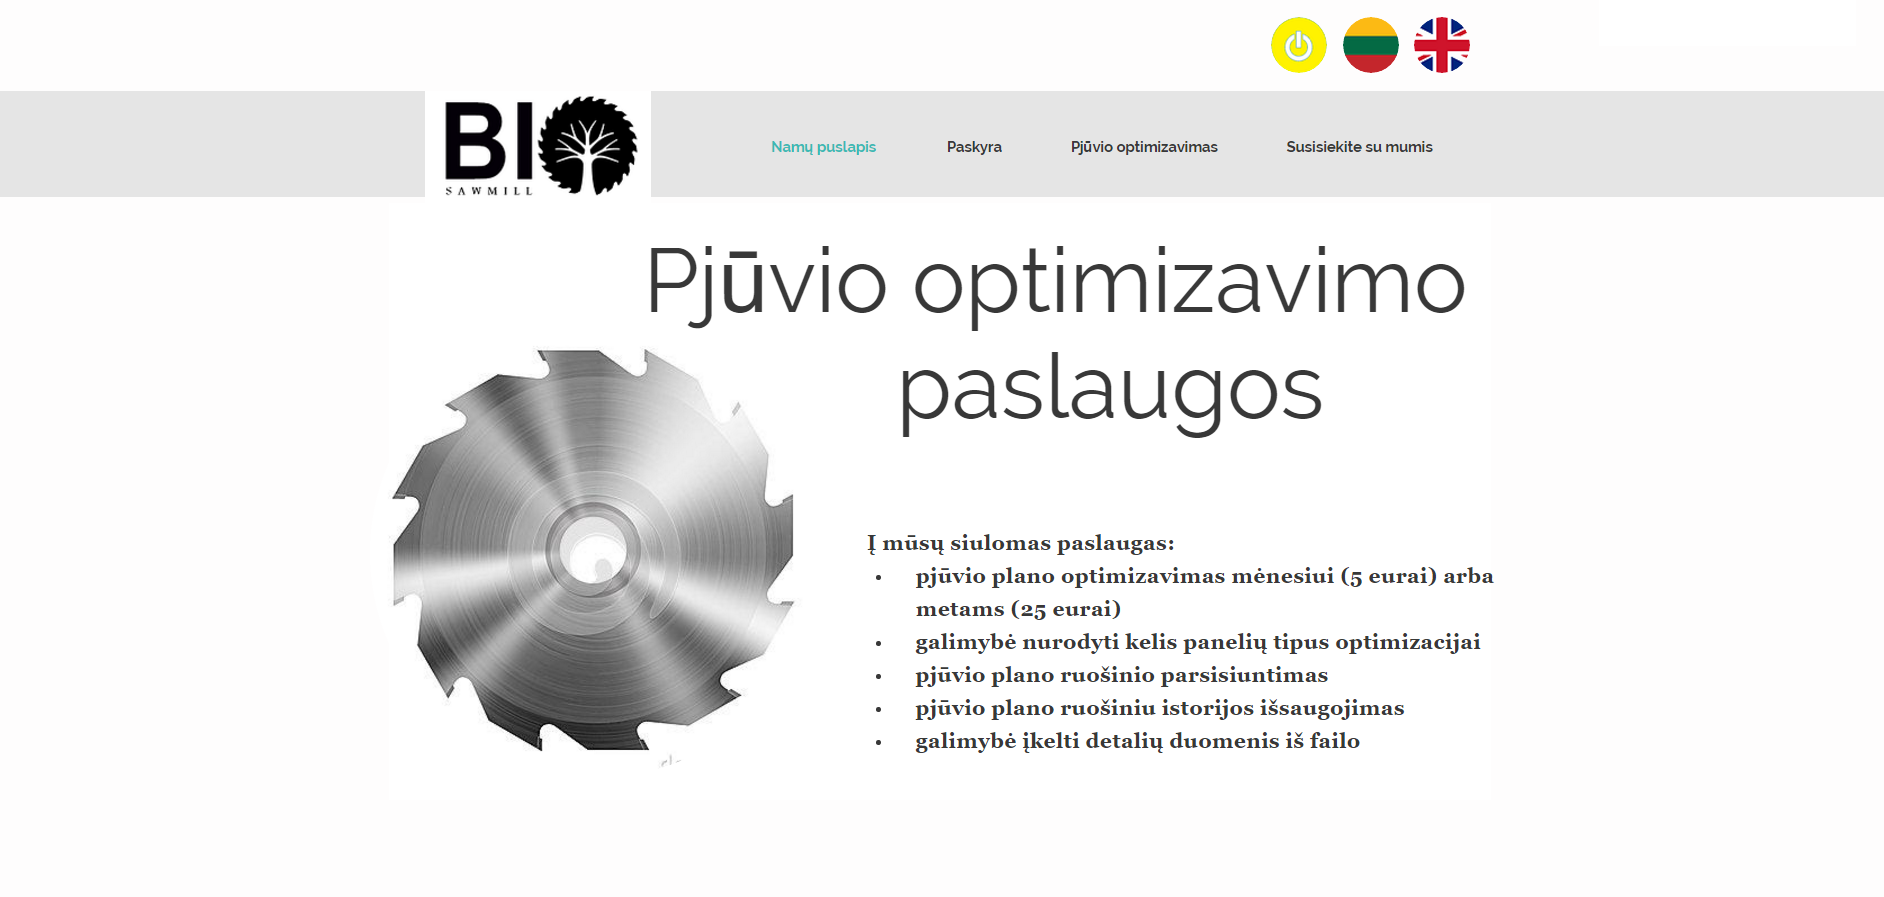
\includegraphics[scale=0.5]{interfeisai/pagrindinis}

\subsection{Vartotojo paskyros puslapis}
\hspace{-2cm}
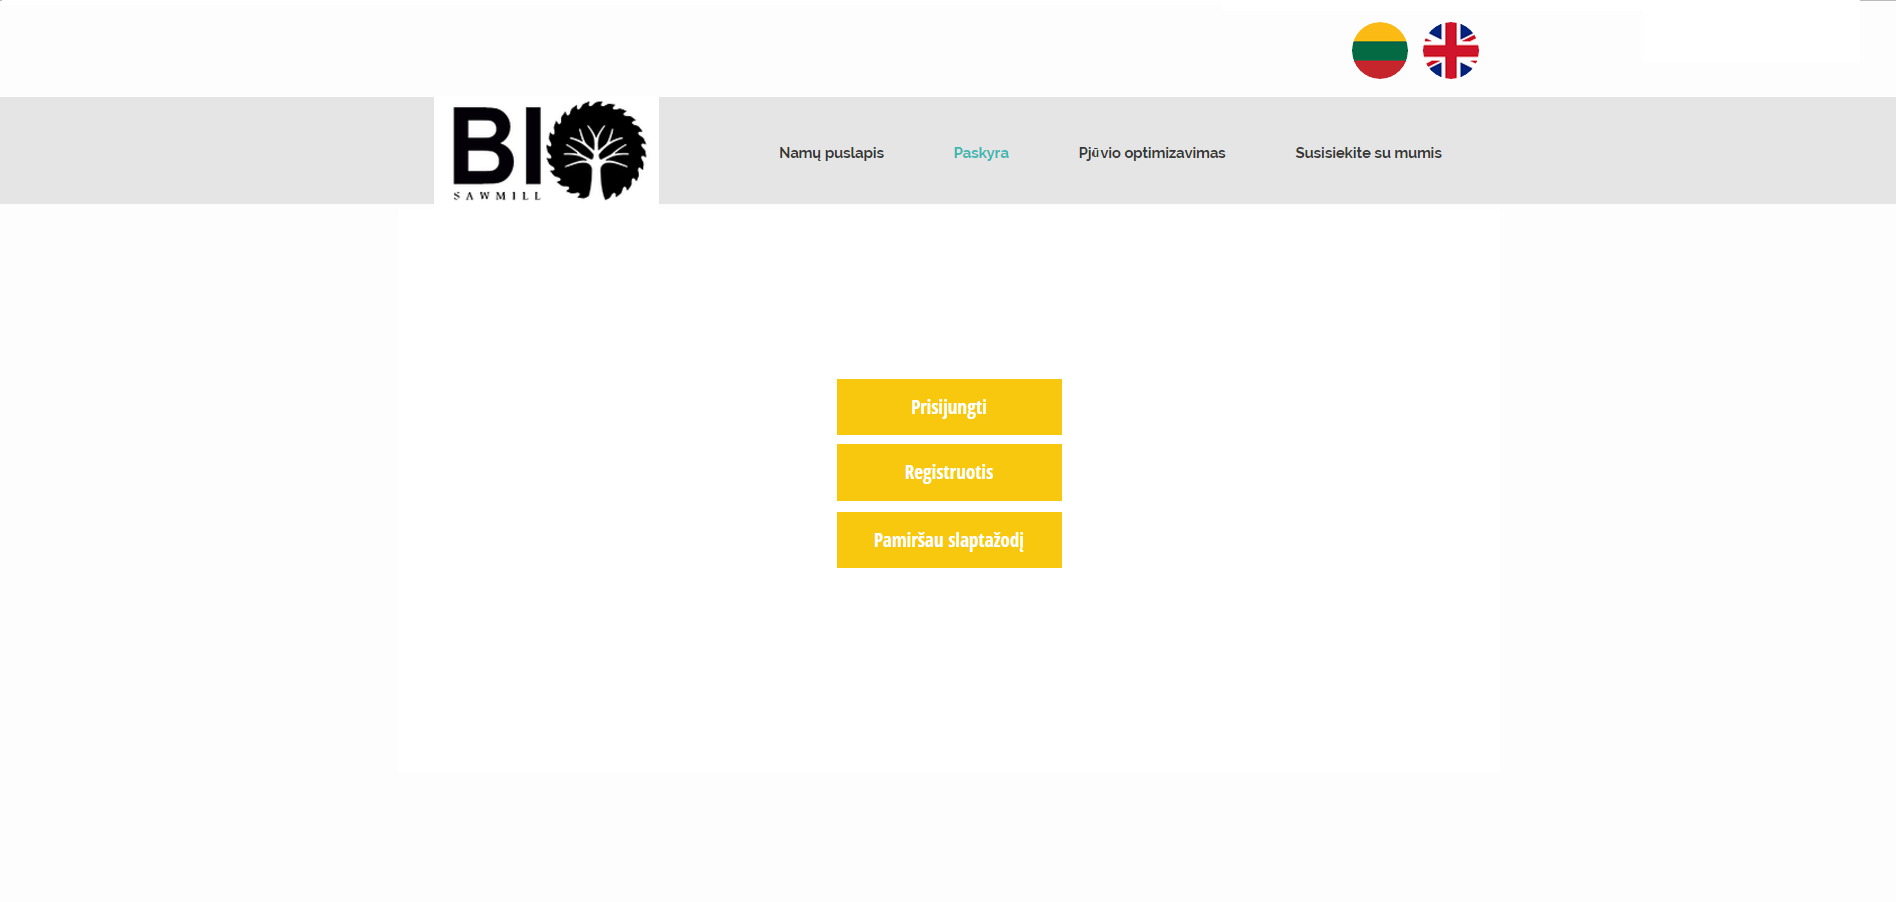
\includegraphics[scale=0.5]{interfeisai/paskyrosPuslapisNeprisijungta}

\subsection{Vartotojo paskyros puslapis - registracija}
\hspace{-2cm}
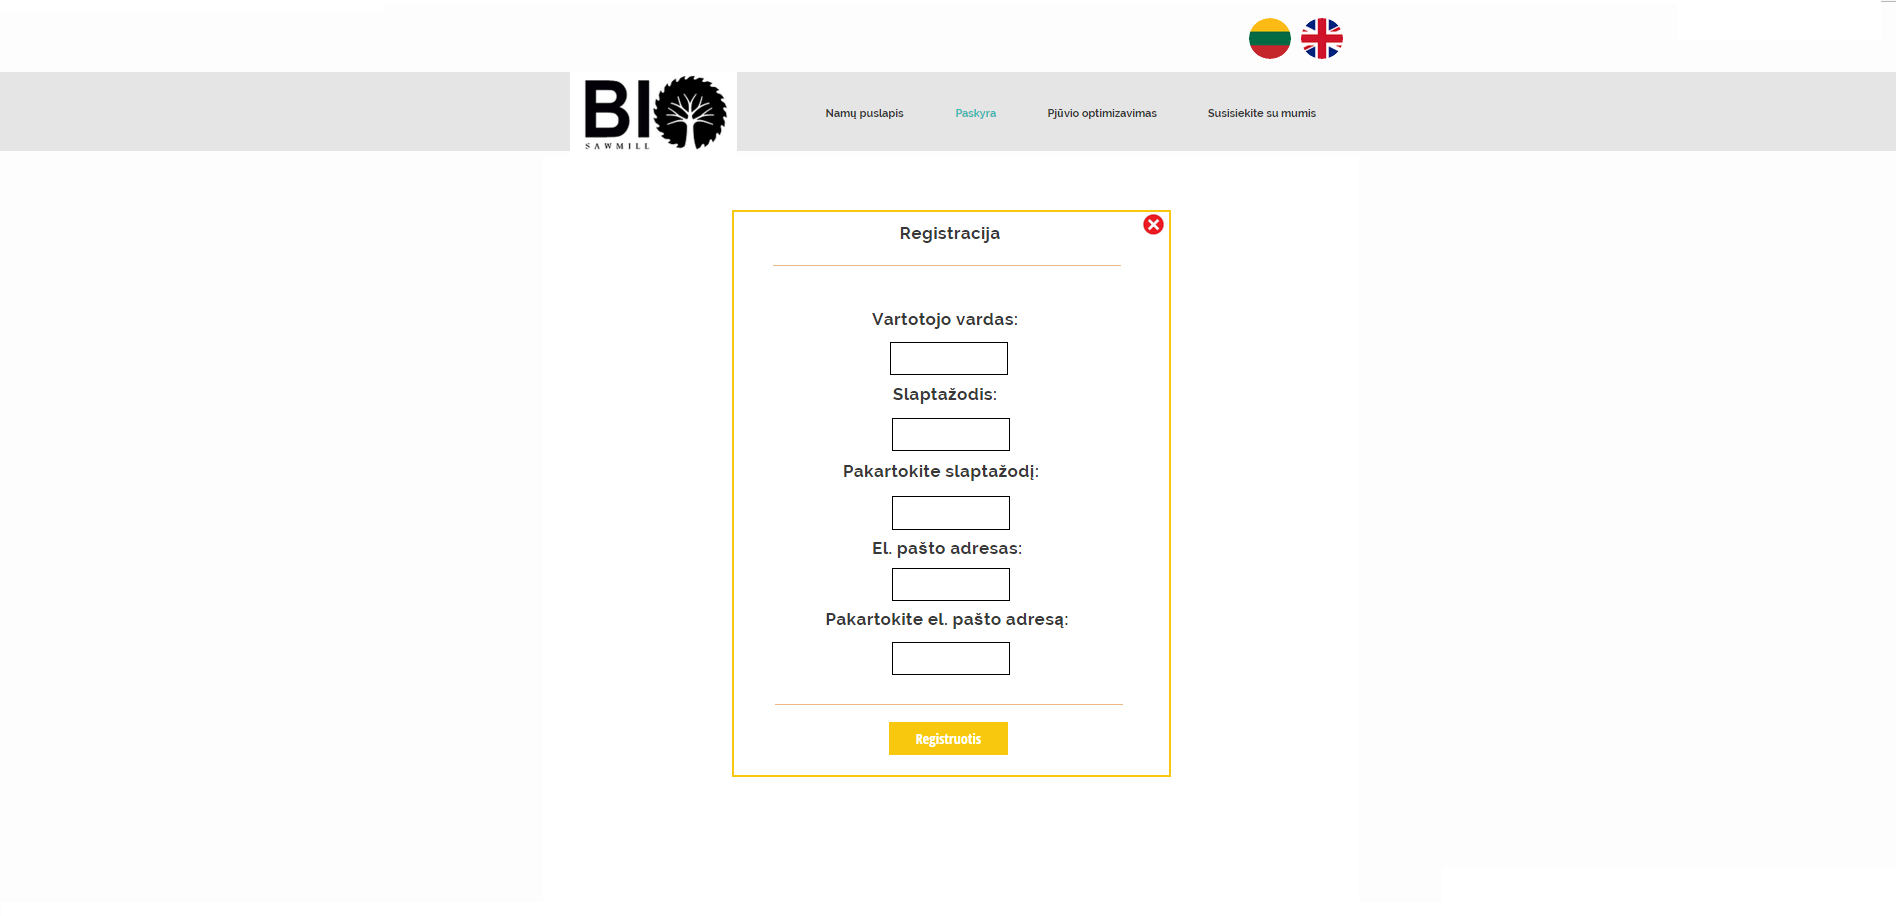
\includegraphics[scale=0.5]{interfeisai/paskyrosPuslapisRegistracija}

\subsection{Vartotojo paskyros puslapis - registracija (su klaida)}
\hspace{-2cm}
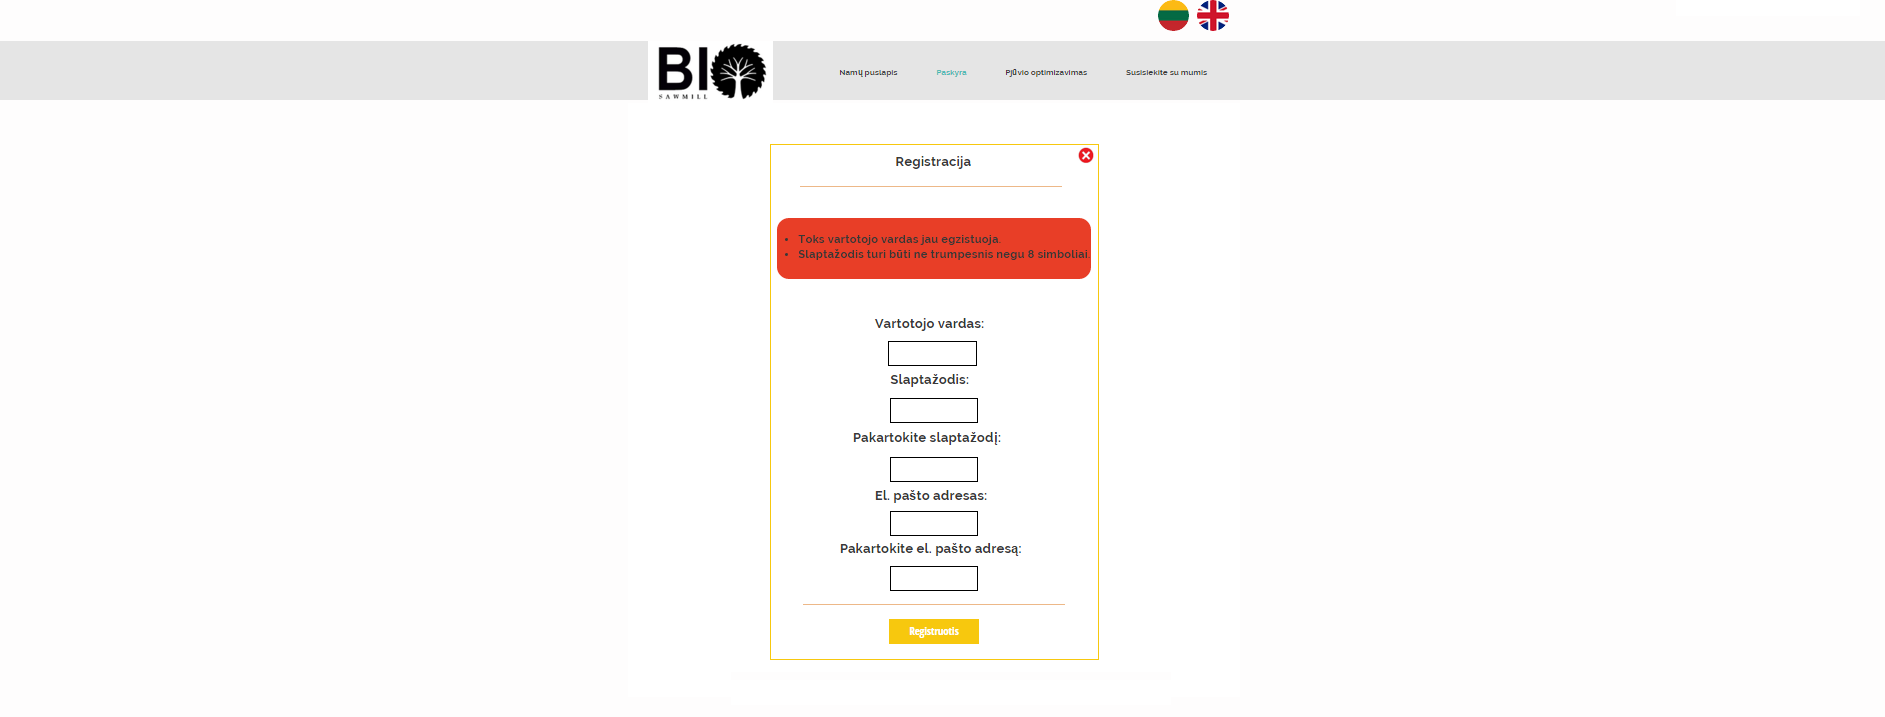
\includegraphics[scale=0.5]{interfeisai/paskyrosPuslapisRegistracijaSuKlaida}

\subsection{Vartotojo paskyros puslapis - sėkminga registracija}
\hspace{-2cm}
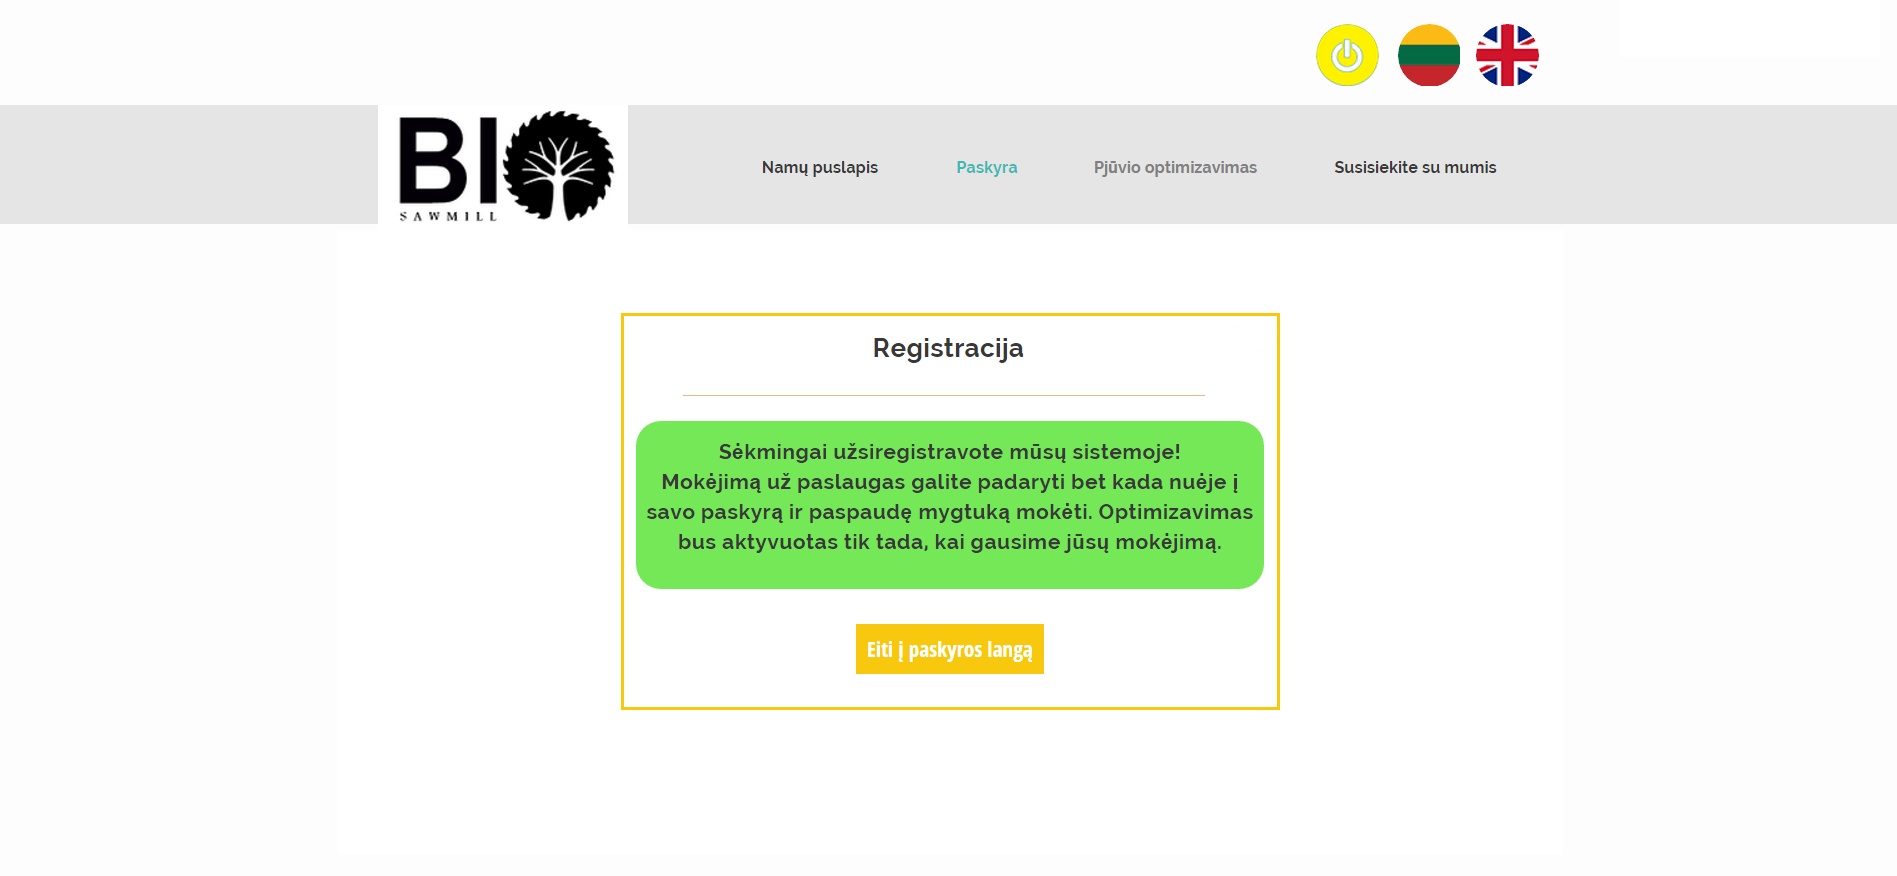
\includegraphics[scale=0.5]{interfeisai/paskyrosPuslapisRegistracijaSekminga}

\subsection{Vartotojo paskyros puslapis - prisijungimas}
\hspace{-2cm}
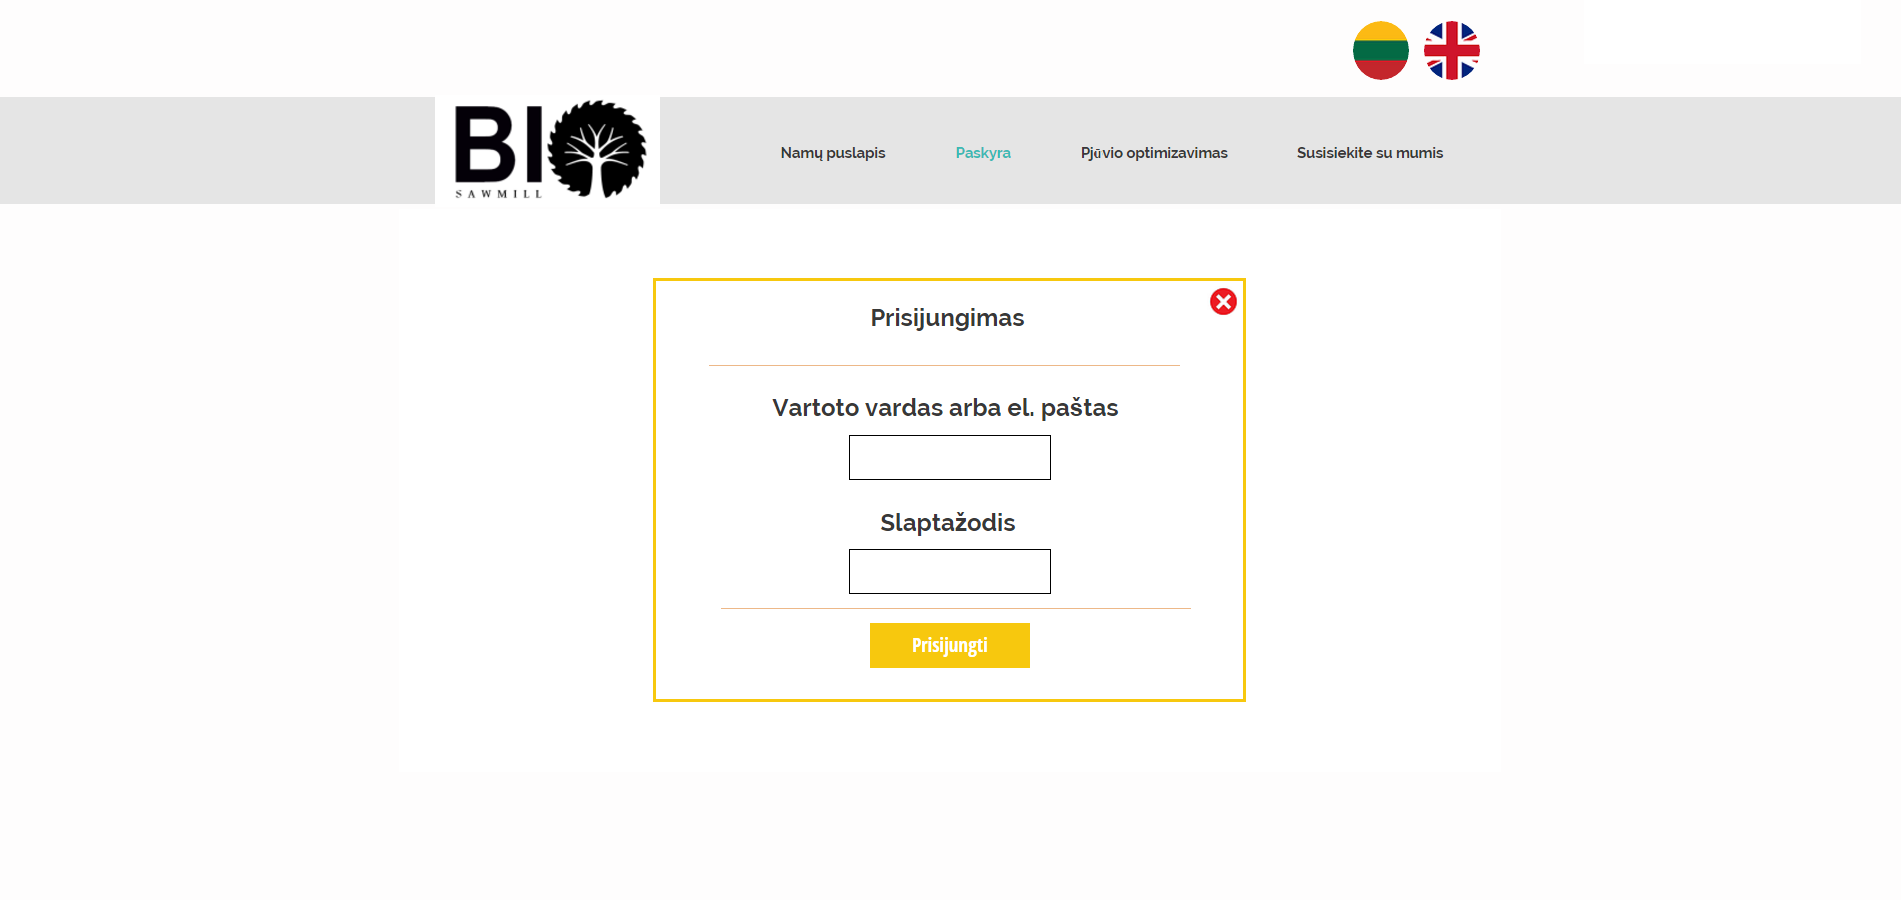
\includegraphics[scale=0.5]{interfeisai/paskyrosPuslapisPrisijungimas}

\subsection{Vartotojo paskyros puslapis - prisijungimas (su klaida)}
\hspace{-2cm}
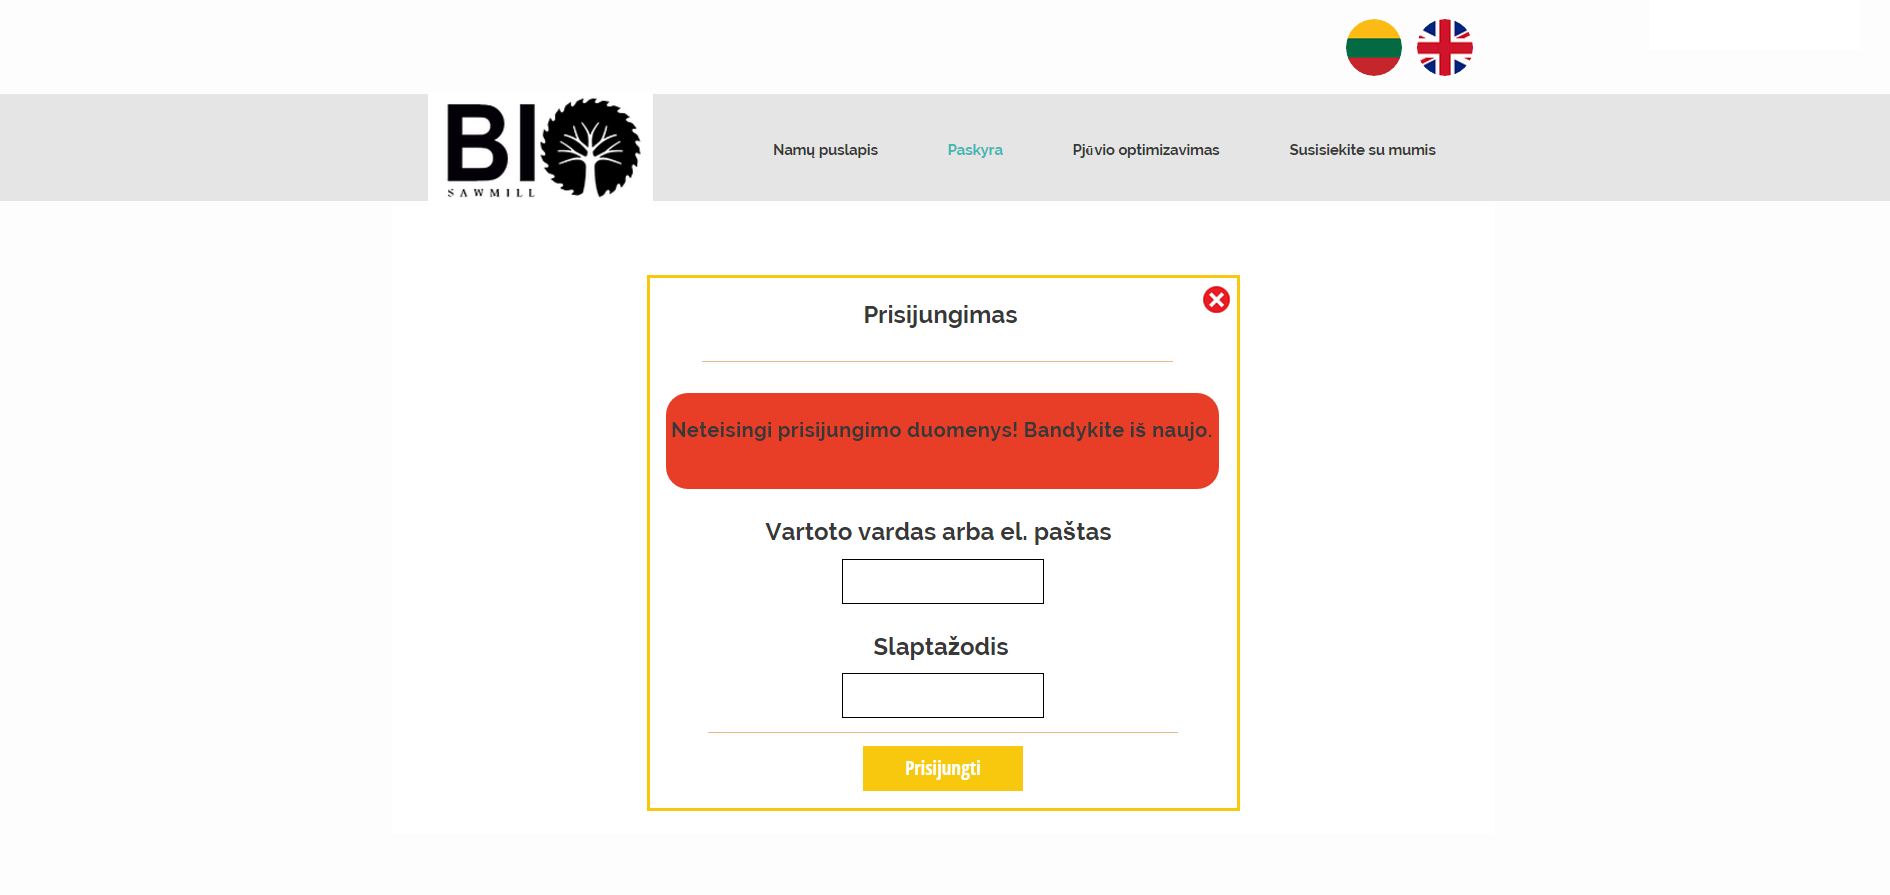
\includegraphics[scale=0.5]{interfeisai/paskyrosPuslapisPrisijungimasSuKlaida}

\subsection{Vartotojo paskyros puslapis - pamirštas slaptažodis}
\hspace{-2cm}
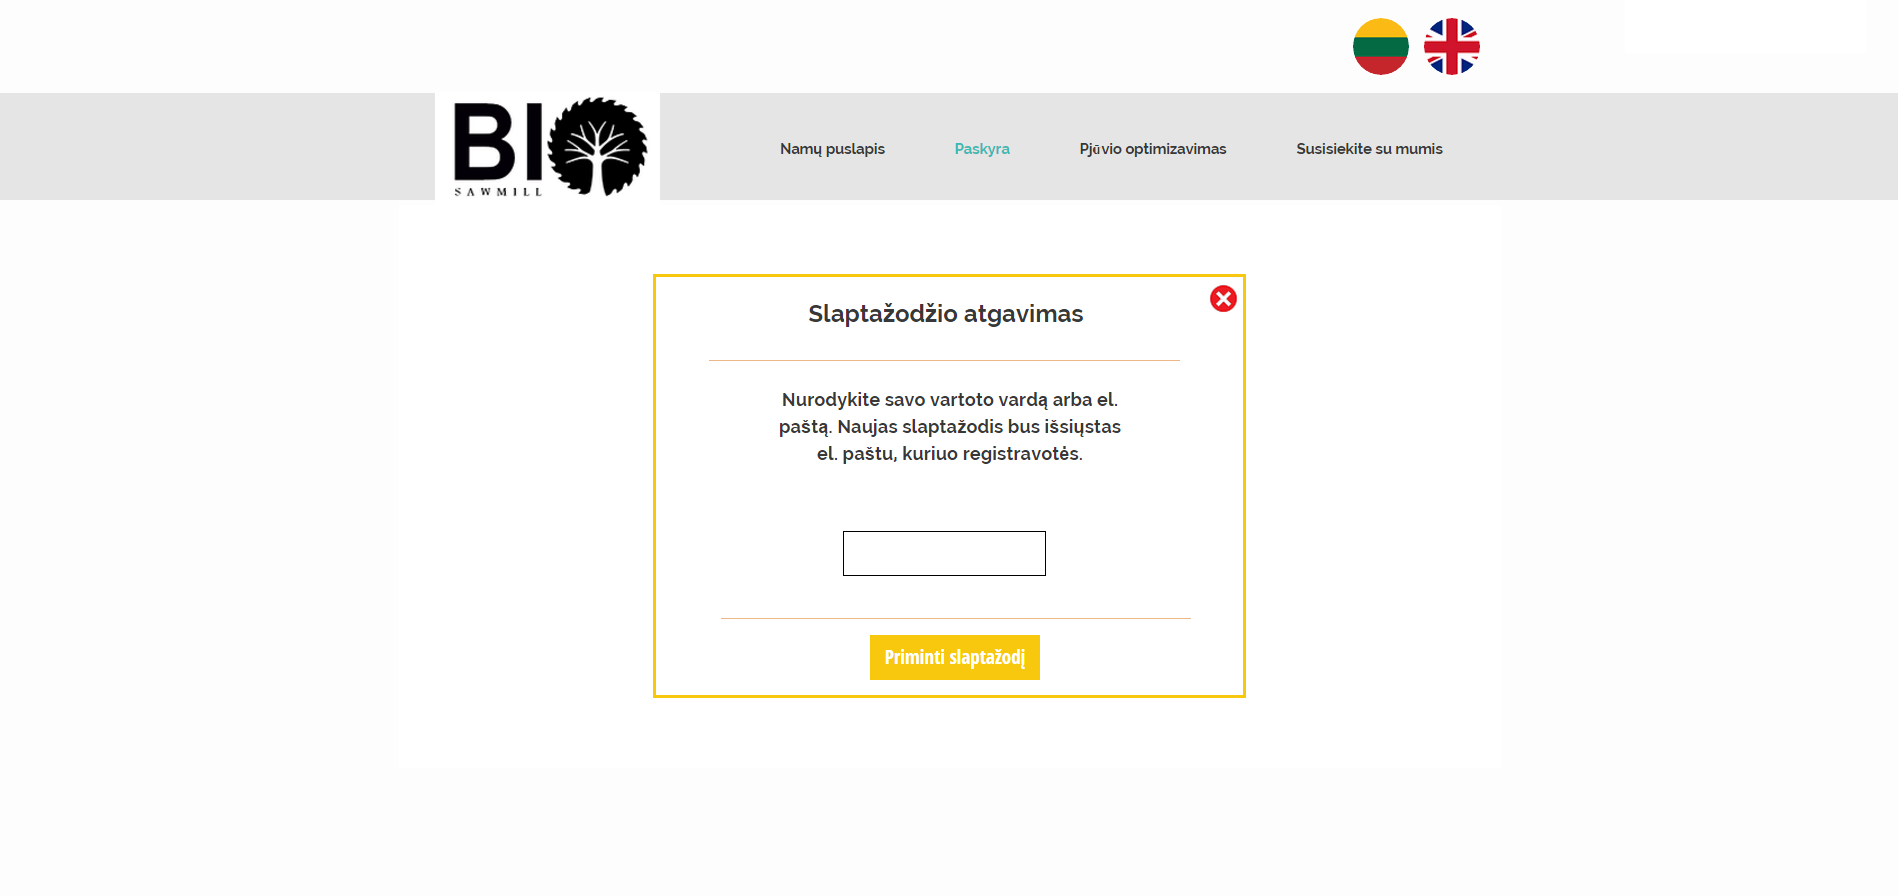
\includegraphics[scale=0.5]{interfeisai/paskyrosPuslapisPamirstasSlaptazodis}

\subsection{Vartotojo paskyros puslapis - pamirštas slaptažodis 2}
\hspace{-2cm}
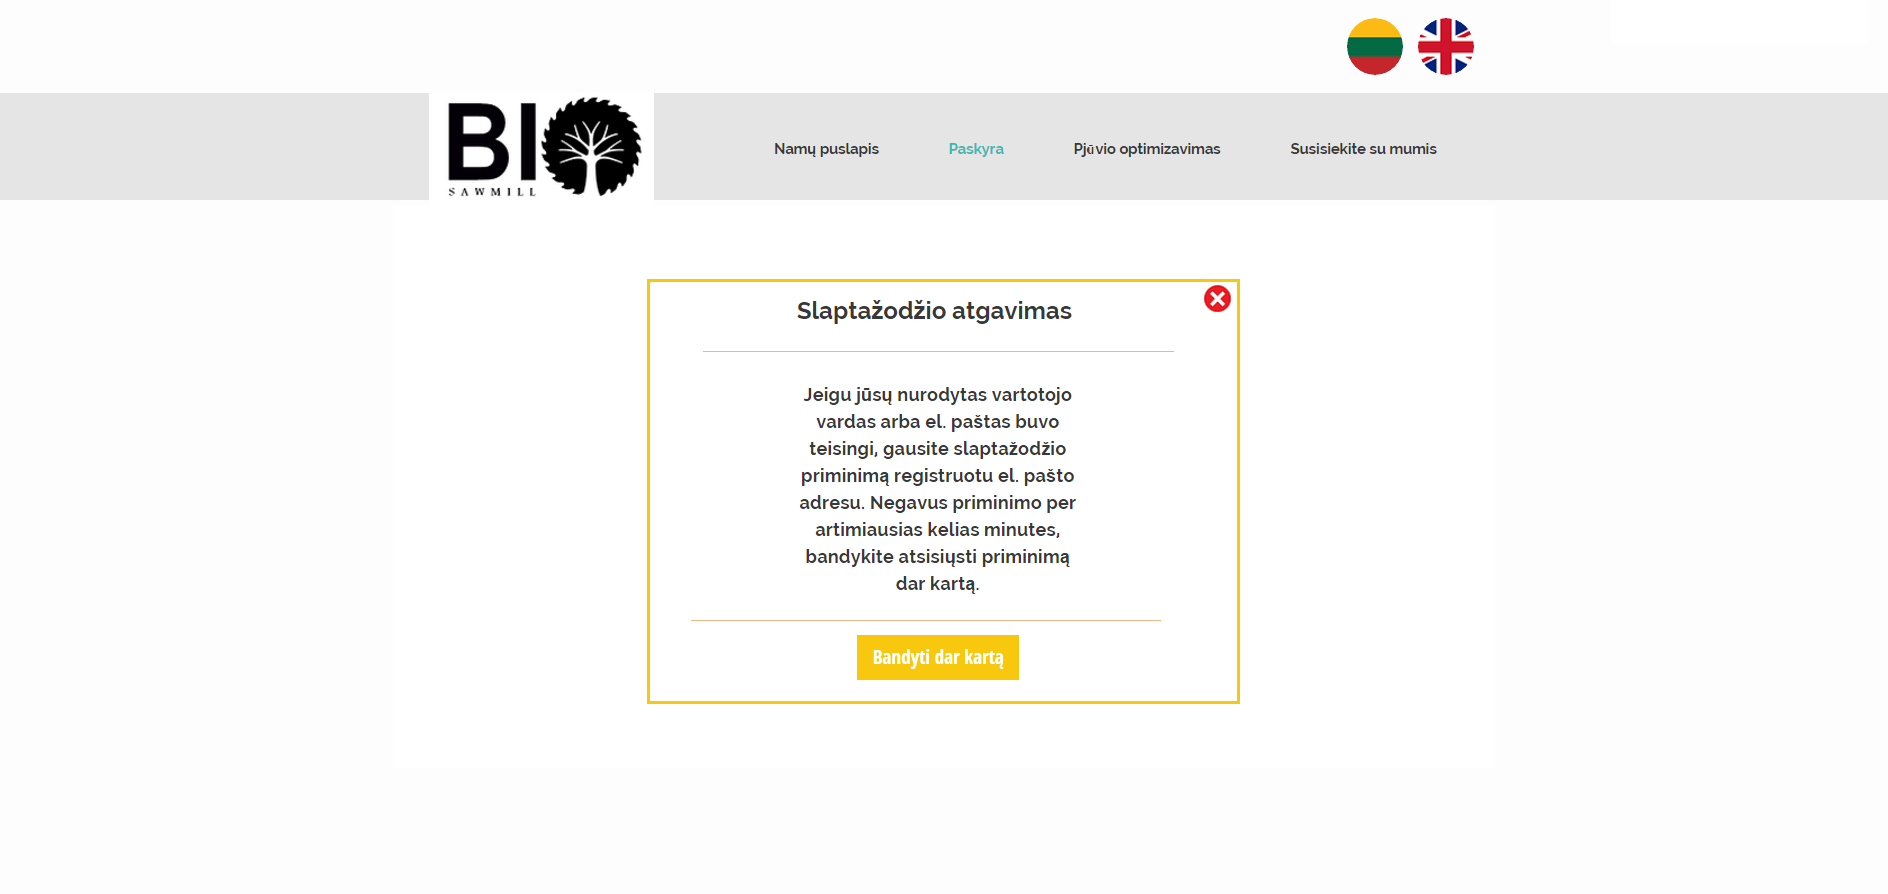
\includegraphics[scale=0.5]{interfeisai/paskyrosPuslapisPamirstasSlaptazodis2}

\subsection{Vartotojo paskyros puslapis - prisijungus (neapmokėta už paslaugas)}
\hspace{-2cm}
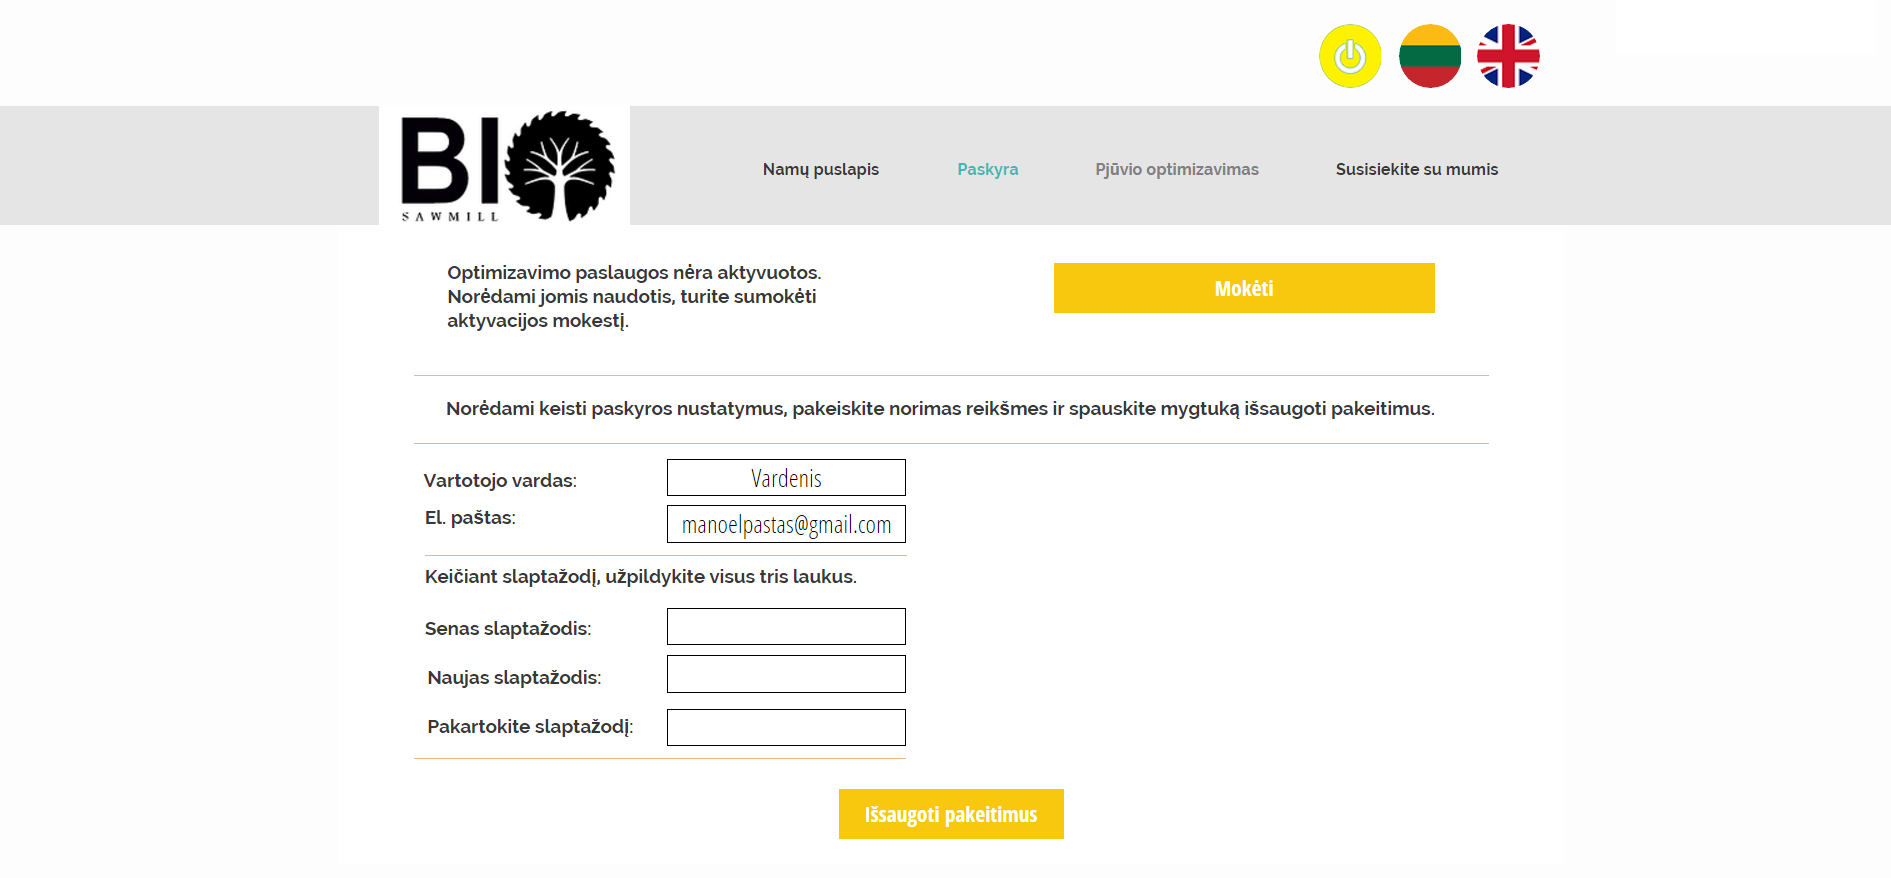
\includegraphics[scale=0.5]{interfeisai/paskyrosPuslapisVartotojasNeapmoketas}

\subsection{Vartotojo paskyros puslapis - prisijungus (apmokėta už paslaugas)}
\hspace{-2cm}
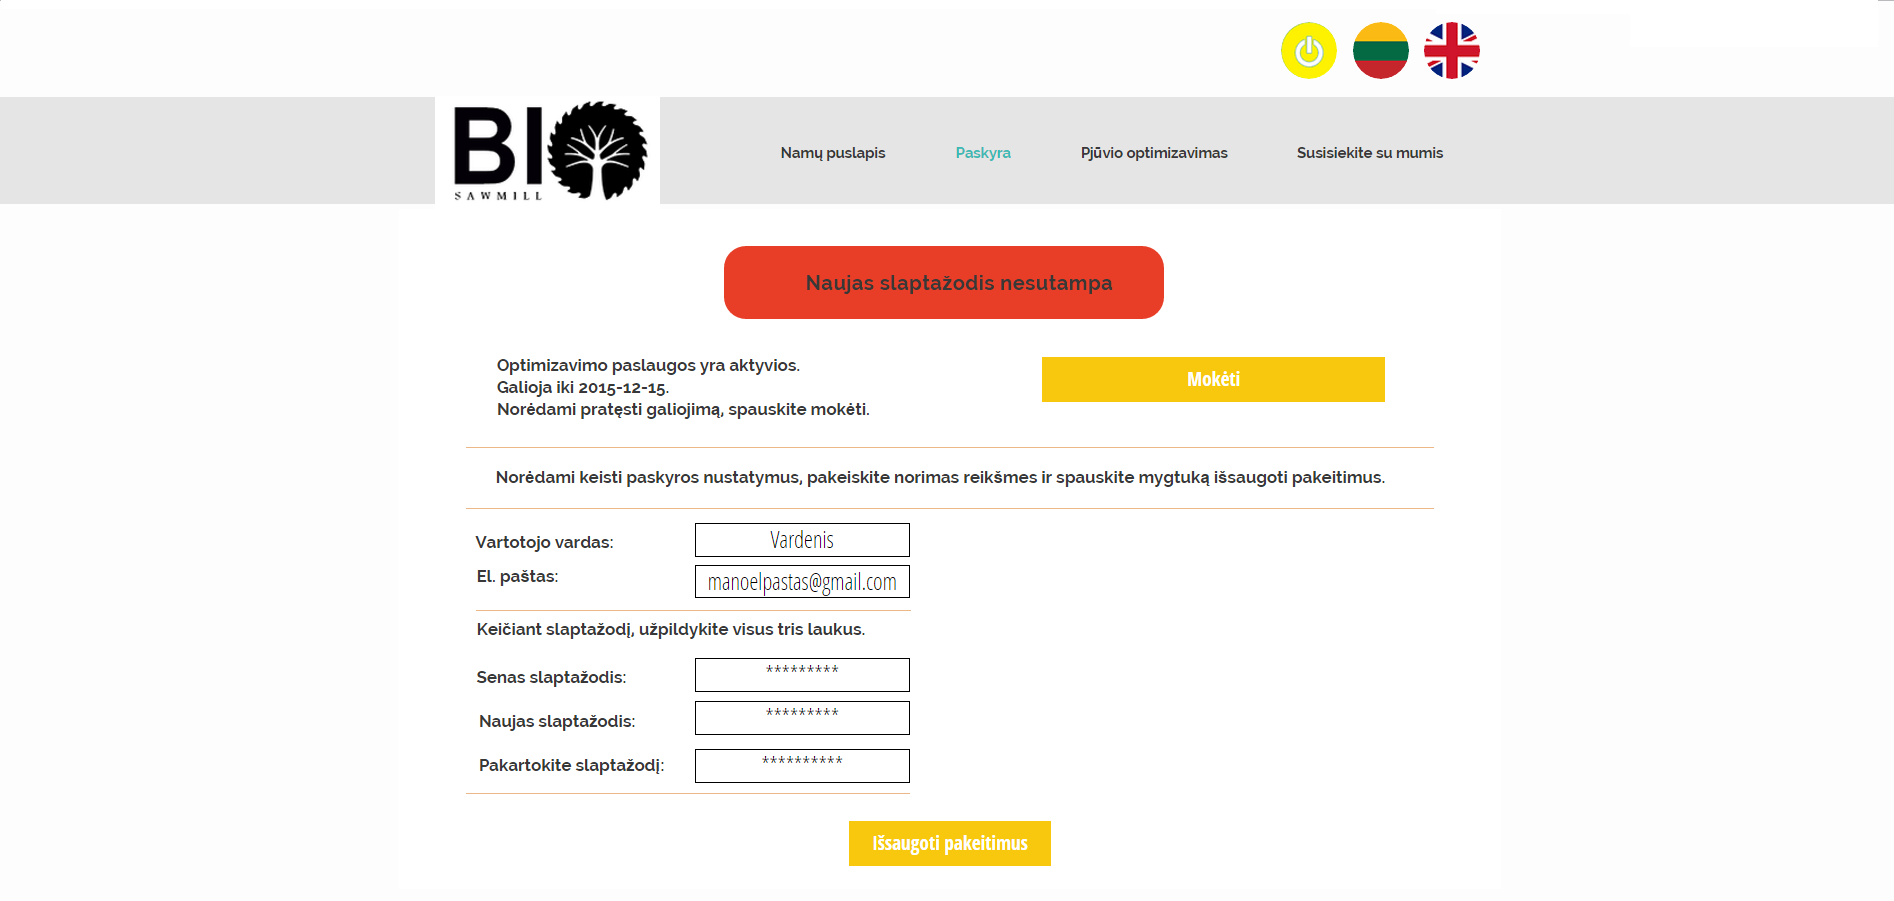
\includegraphics[scale=0.5]{interfeisai/paskyrosPuslapisVartotojasApmoketas}

\subsection{Vartotojo paskyros puslapis - prisijungus - mokėjimas}
\hspace{-2cm}
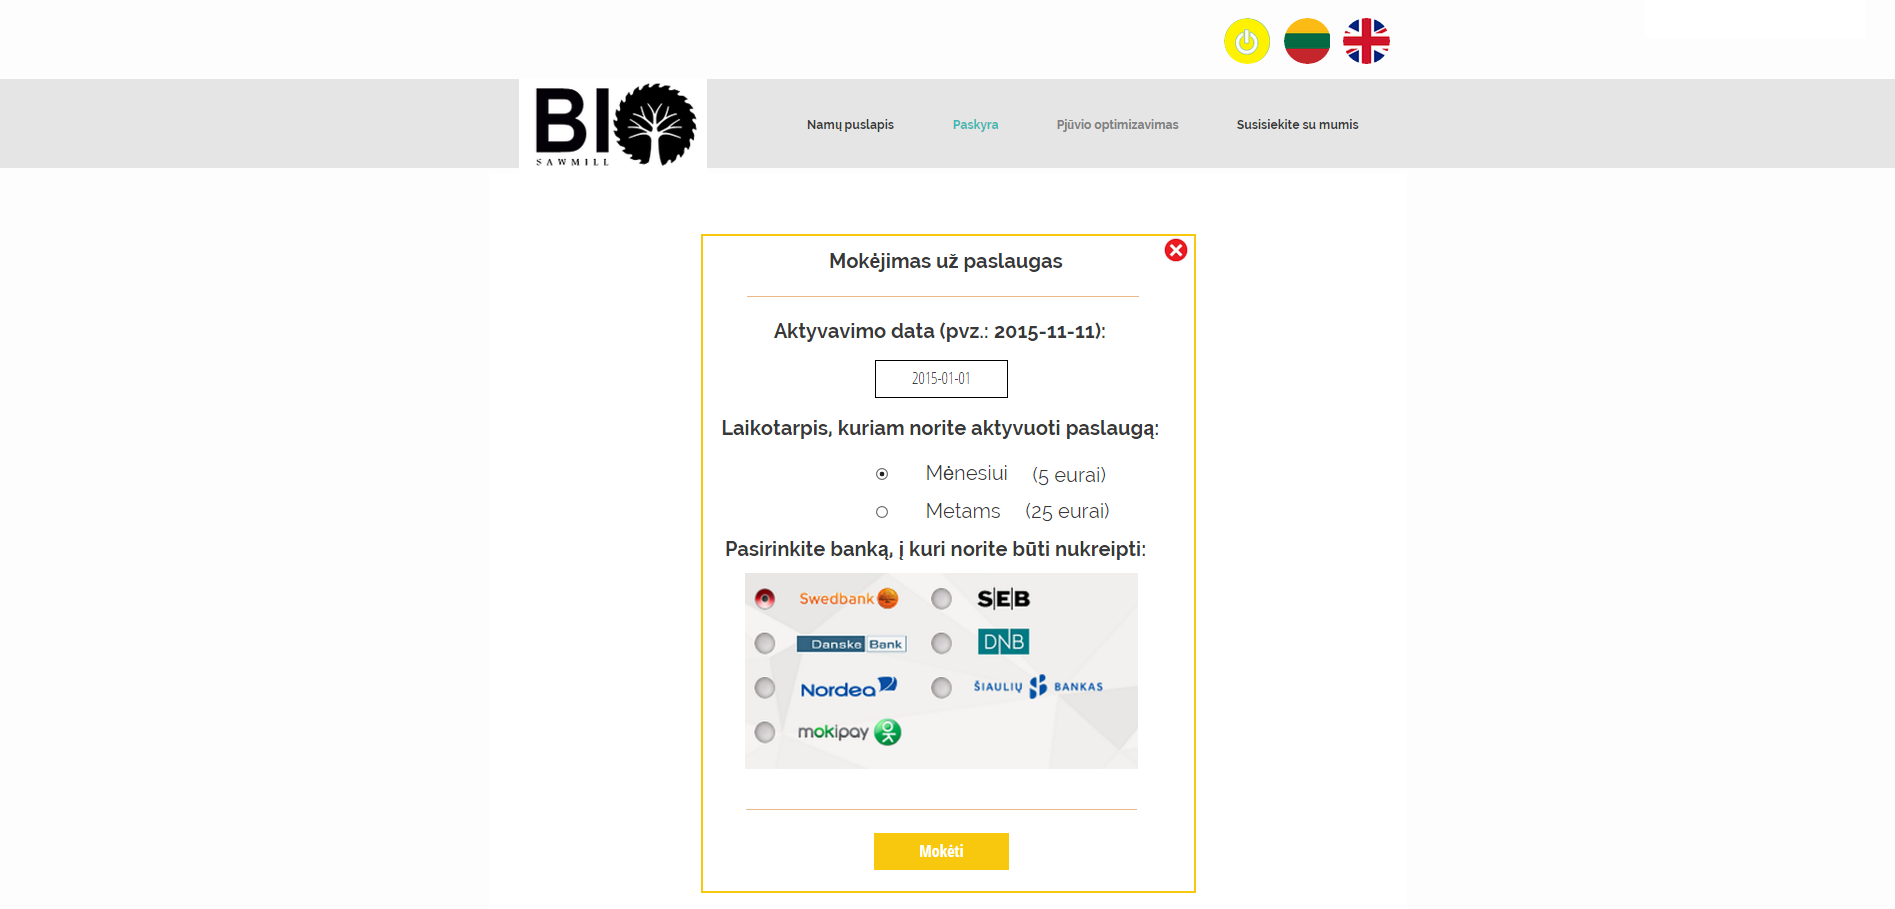
\includegraphics[scale=0.5]{interfeisai/paskyrosPuslapisVartotojasMokejimas}

\subsection{Vartotojo paskyros puslapis - prisijungus - mokėjimas (su klaida)}
\hspace{-2cm}
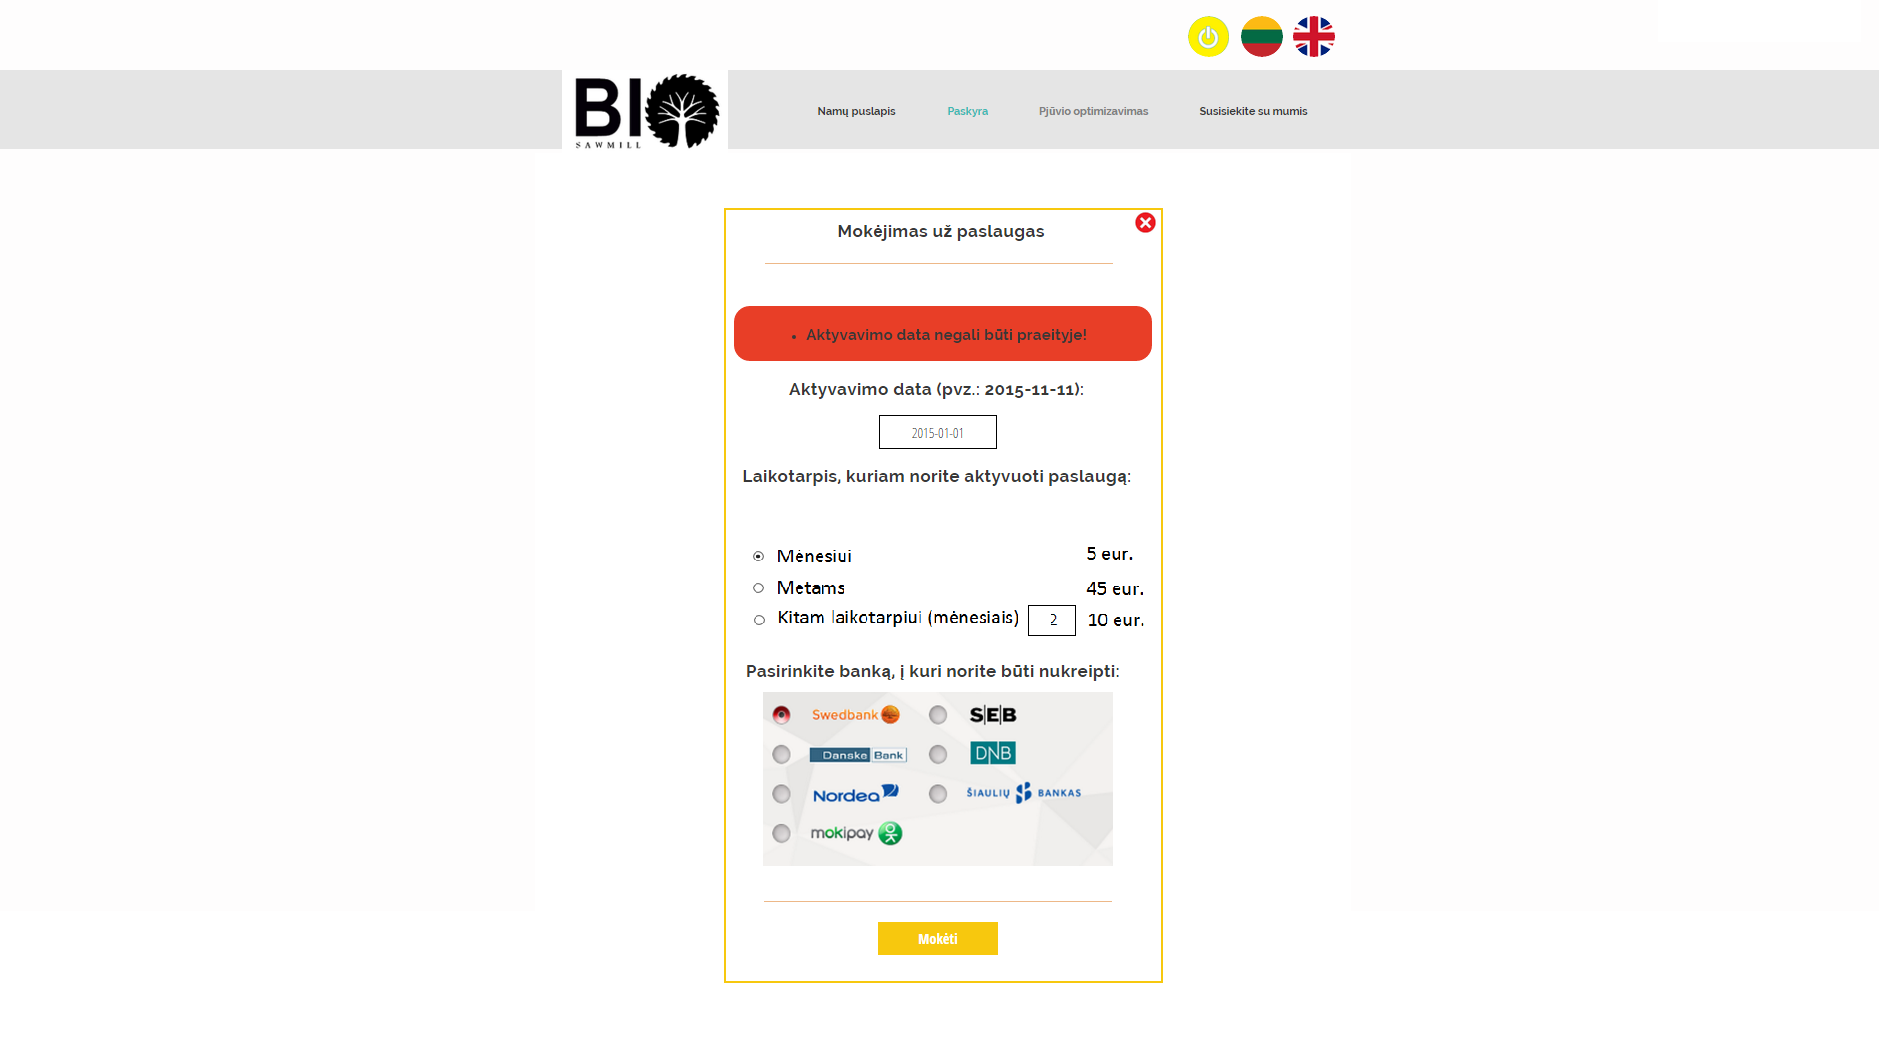
\includegraphics[scale=0.5]{interfeisai/paskyrosPuslapisVartotojasMokejimasSuKlaida}

\subsection{Vartotojo paskyros puslapis - administratorius}
\hspace{-2cm}
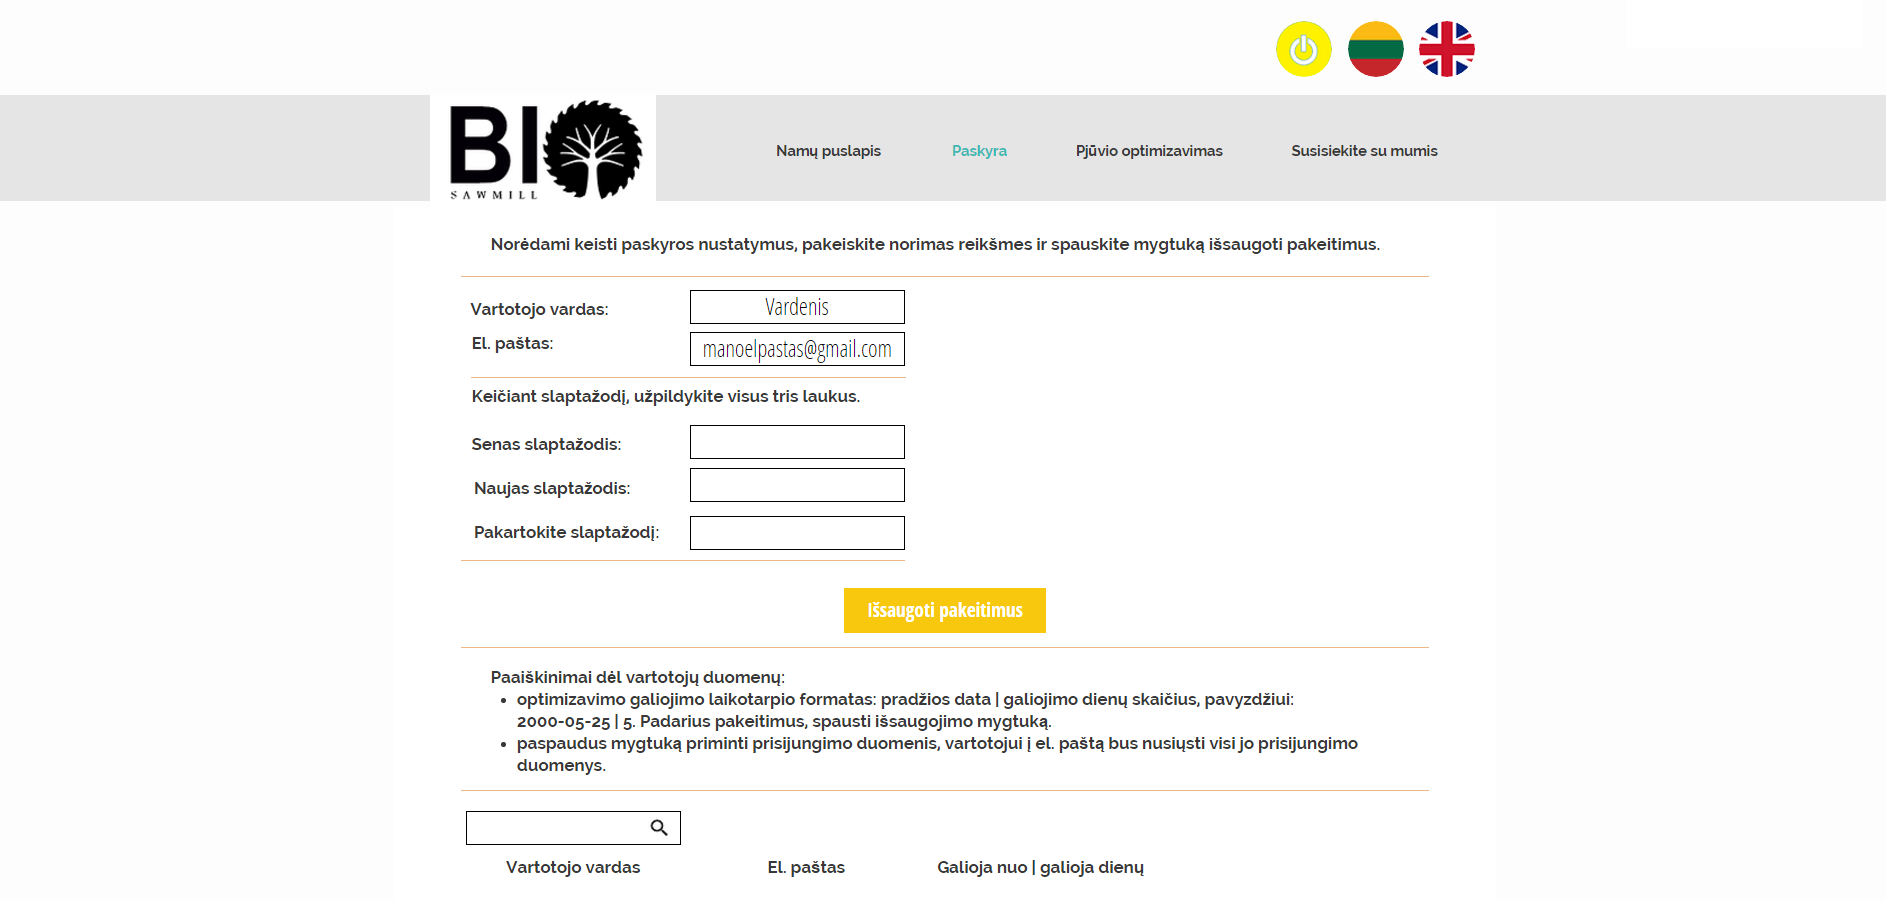
\includegraphics[scale=0.5]{interfeisai/paskyrosPuslapisAdministratorius}

\subsection{Vartotojo paskyros puslapis - administratorius (su klaida)}
\hspace{-2cm}
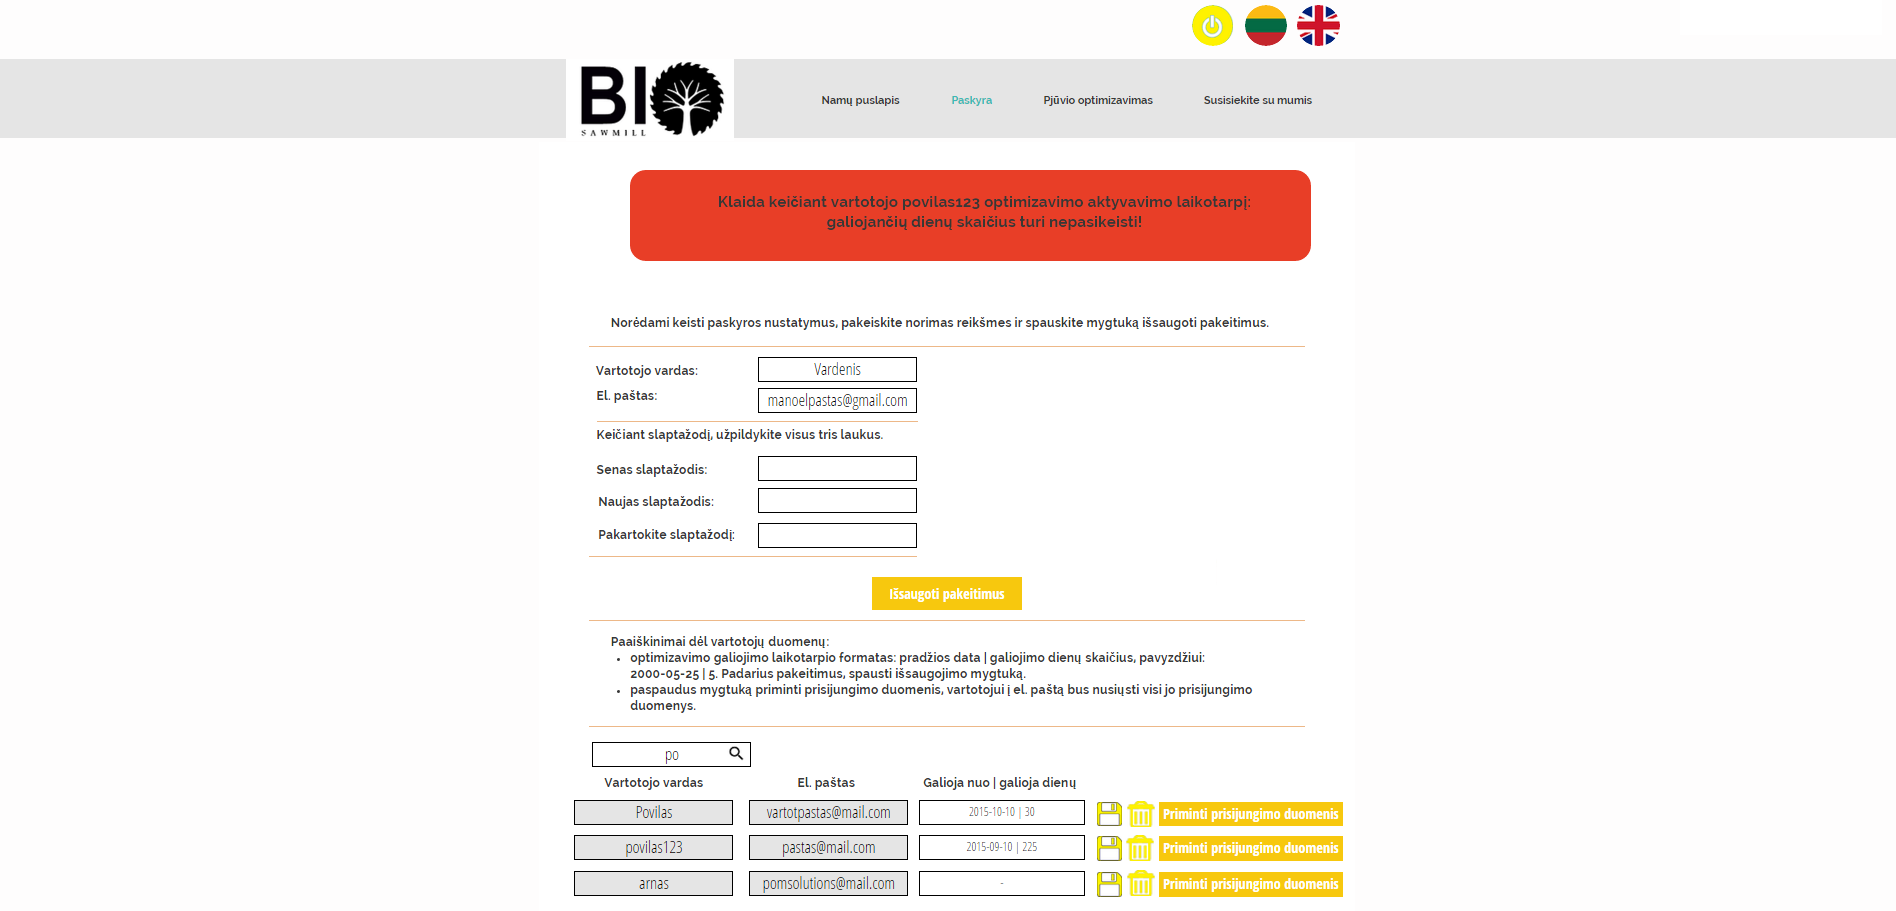
\includegraphics[scale=0.5]{interfeisai/paskyrosPuslapisAdministratoriusSuKlaida}

\subsection{Optimizavimo puslapis - neprisijungus}
\hspace{-2cm}
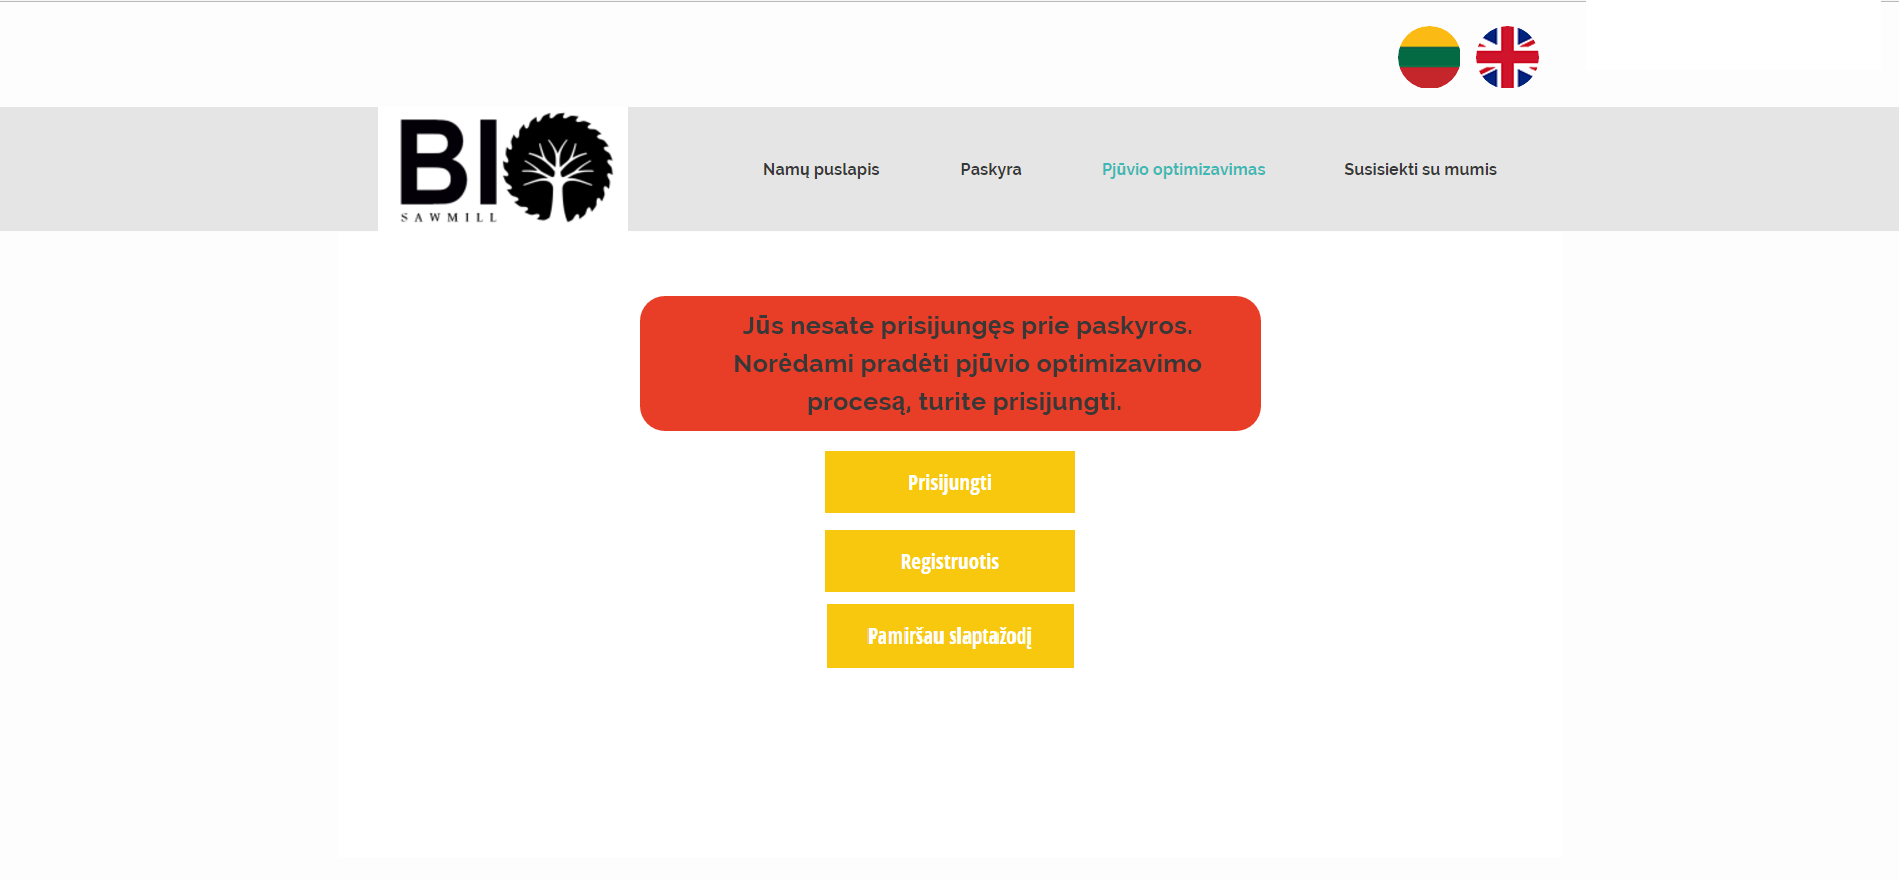
\includegraphics[scale=0.5]{interfeisai/optimizavimoPuslapisNeprisijungus}

\subsection{Optimizavimo puslapis - prisijungus}
\hspace{-2cm}
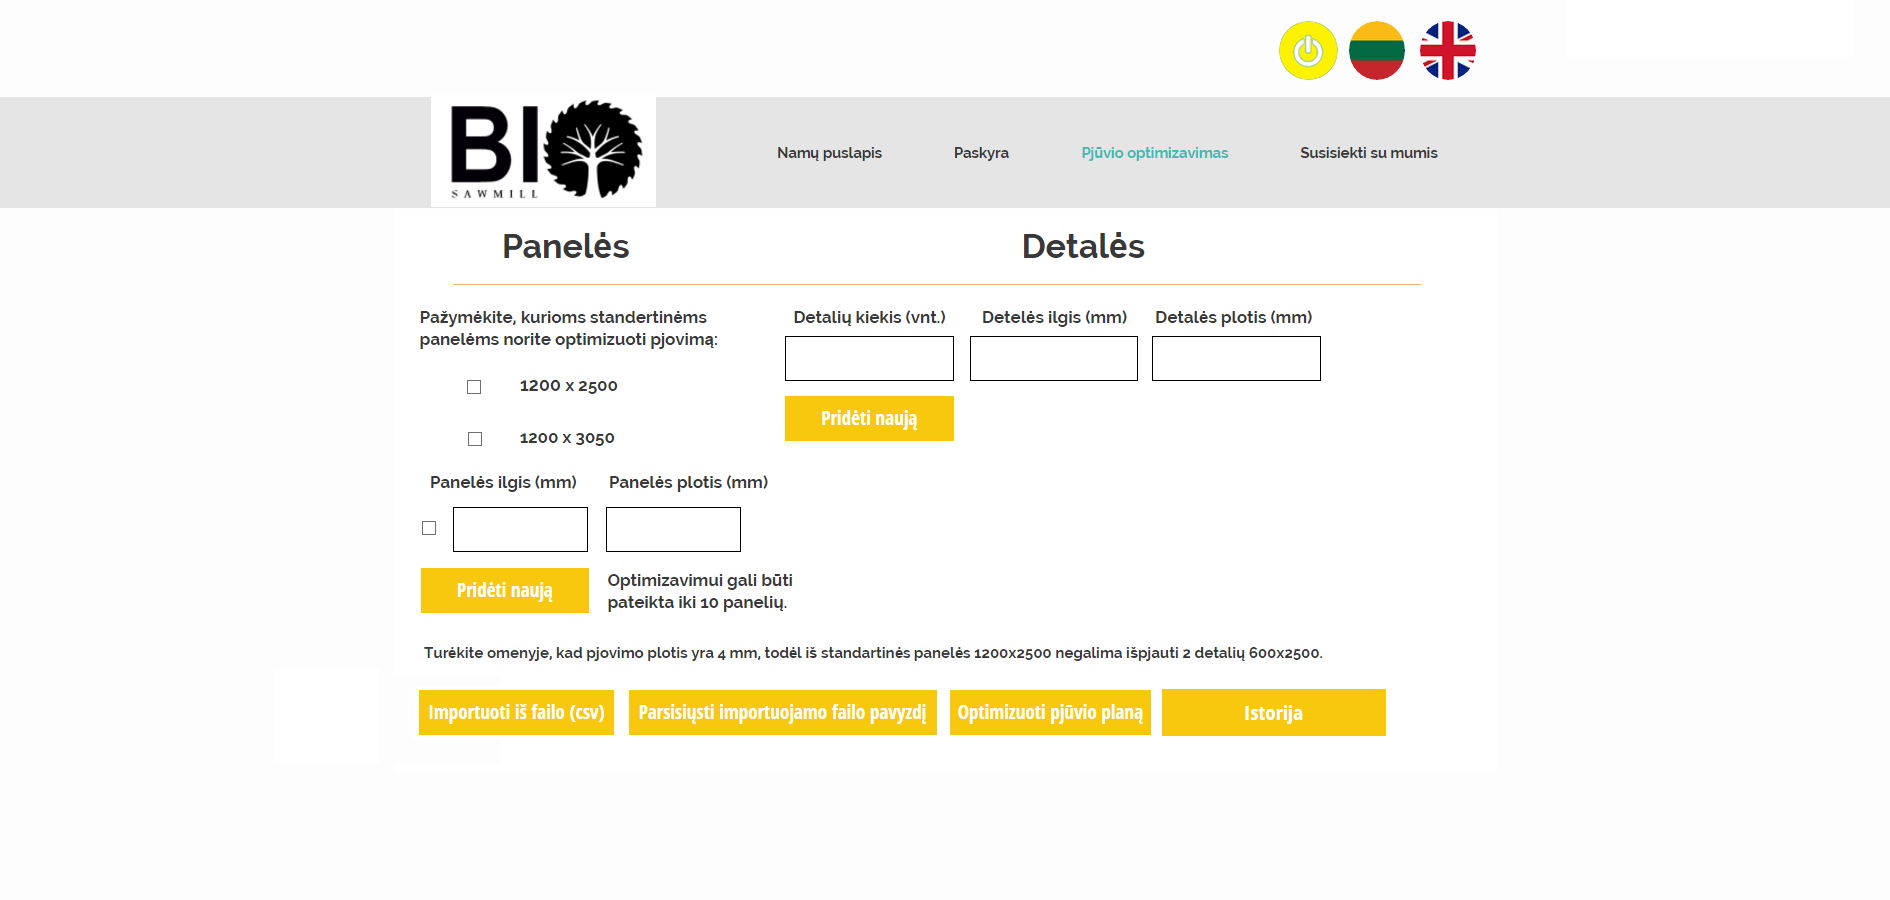
\includegraphics[scale=0.5]{interfeisai/optimizavimoPuslapisPrisijungus}

\subsection{Optimizavimo puslapis - prisijungus (su klaida)}
\hspace{-2cm}
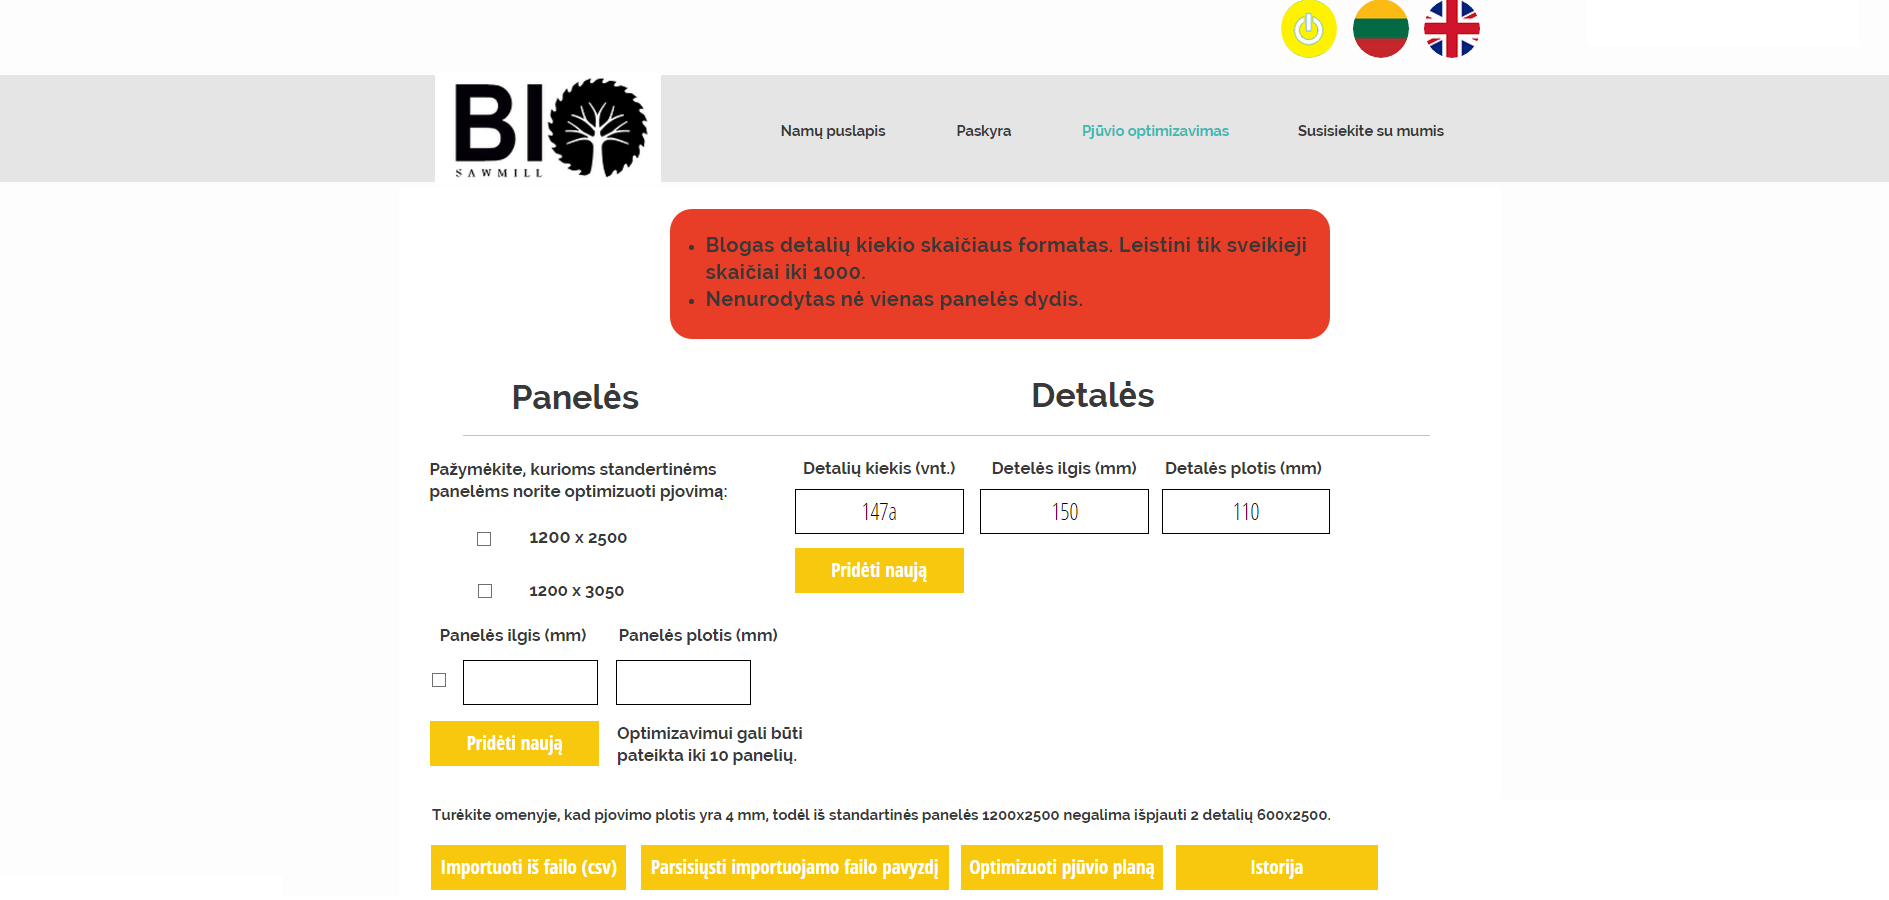
\includegraphics[scale=0.5]{interfeisai/optimizavimoPuslapisPrisijungusSuKlaida}

\subsection{Optimizavimo puslapis - po optimizavimo proceso}
\hspace{-2cm}
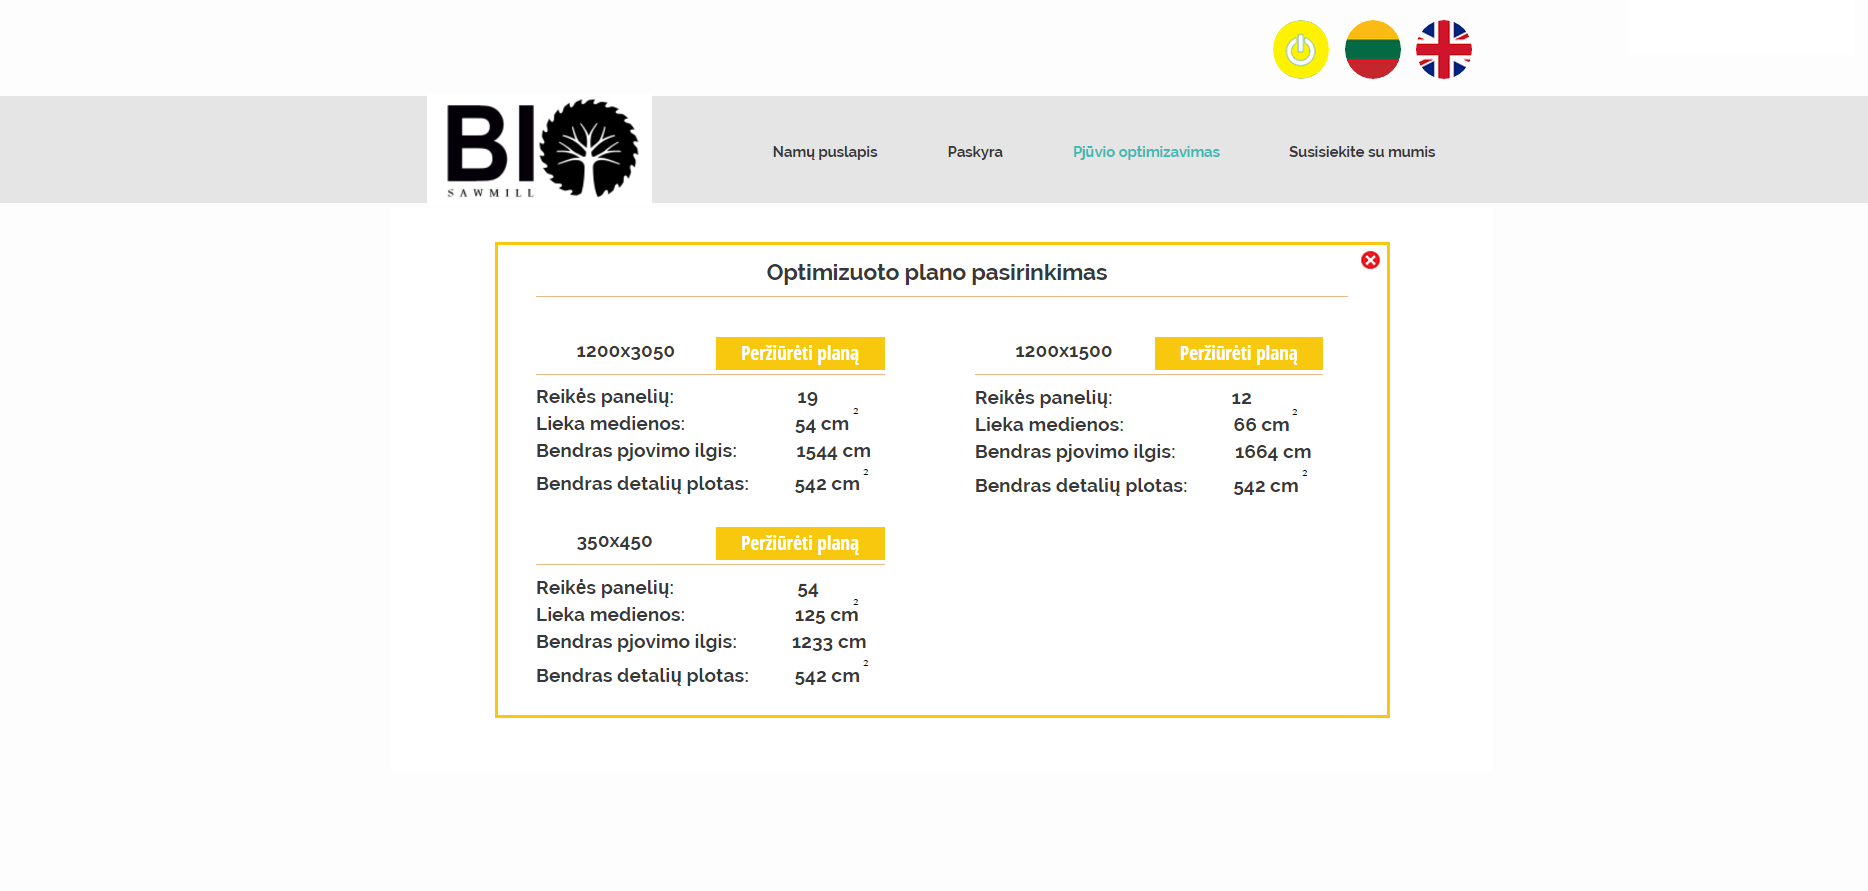
\includegraphics[scale=0.5]{interfeisai/optimizavimoPuslapisOptimizuotiPlanai}

\subsection{Optimizavimo puslapis - po optimizavimo, pasirinkus vieno iš planų peržiūrą}
\hspace{-2cm}
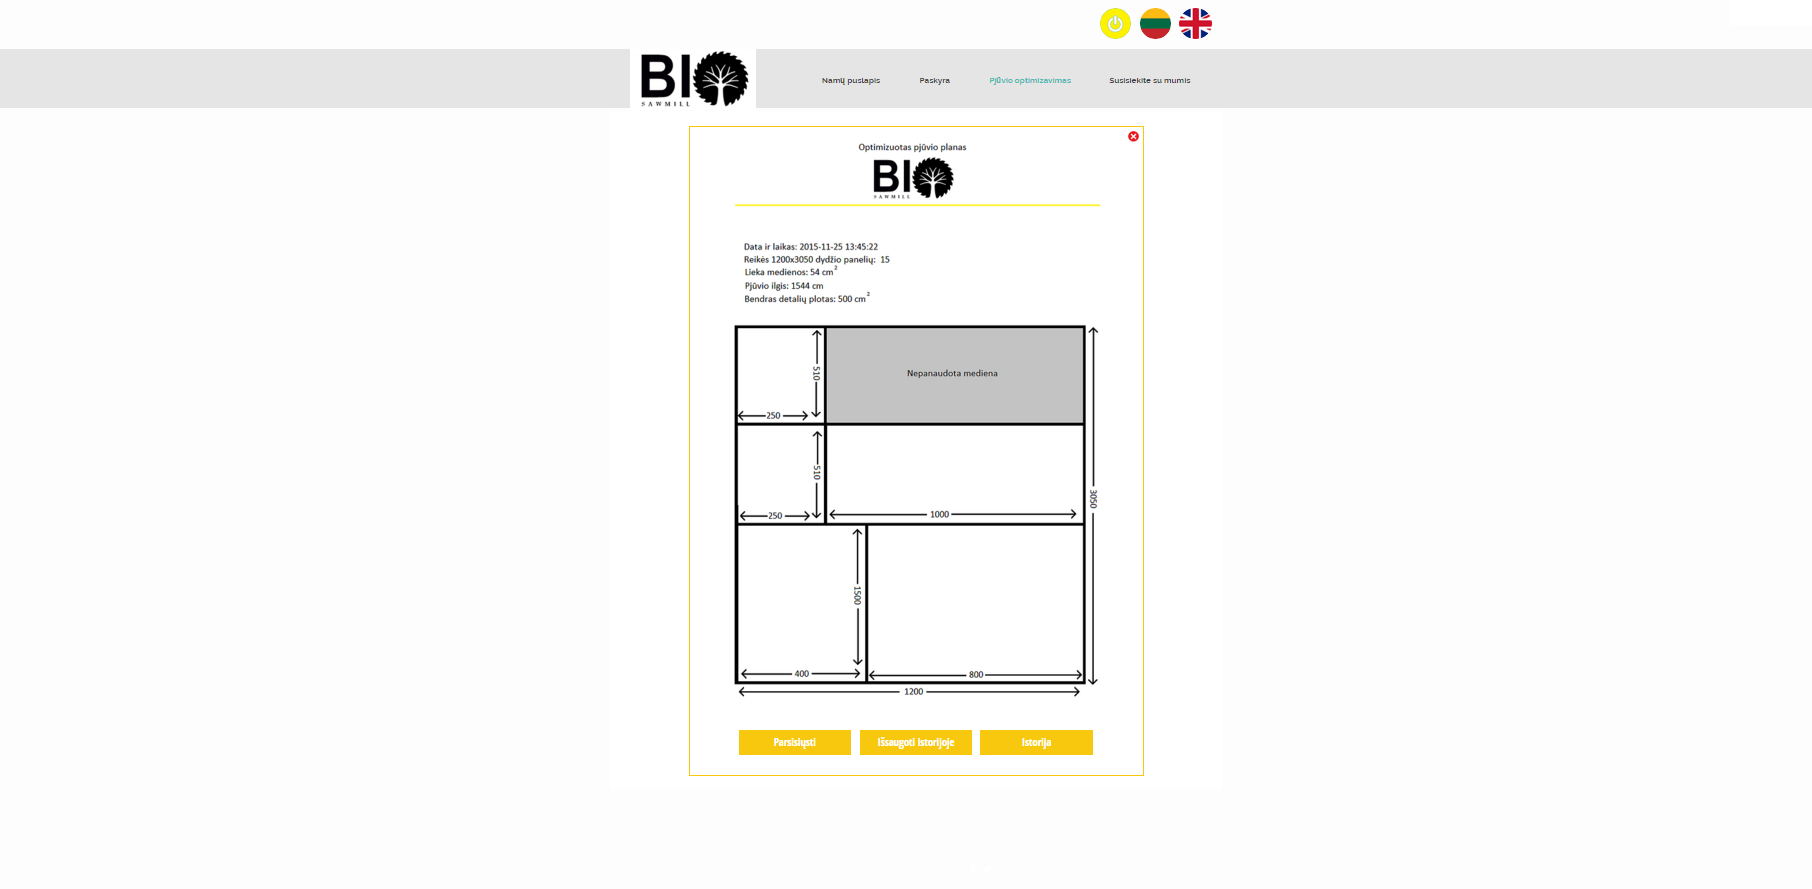
\includegraphics[scale=0.5]{interfeisai/optimizavimoPuslapisPrisijungusPasirinktoPerziura}

\subsection{Optimizavimo puslapis - po optimizavimo, pasirinkus vieno iš planų peržiūrą (iš arčiau)}
\hspace{-2cm}
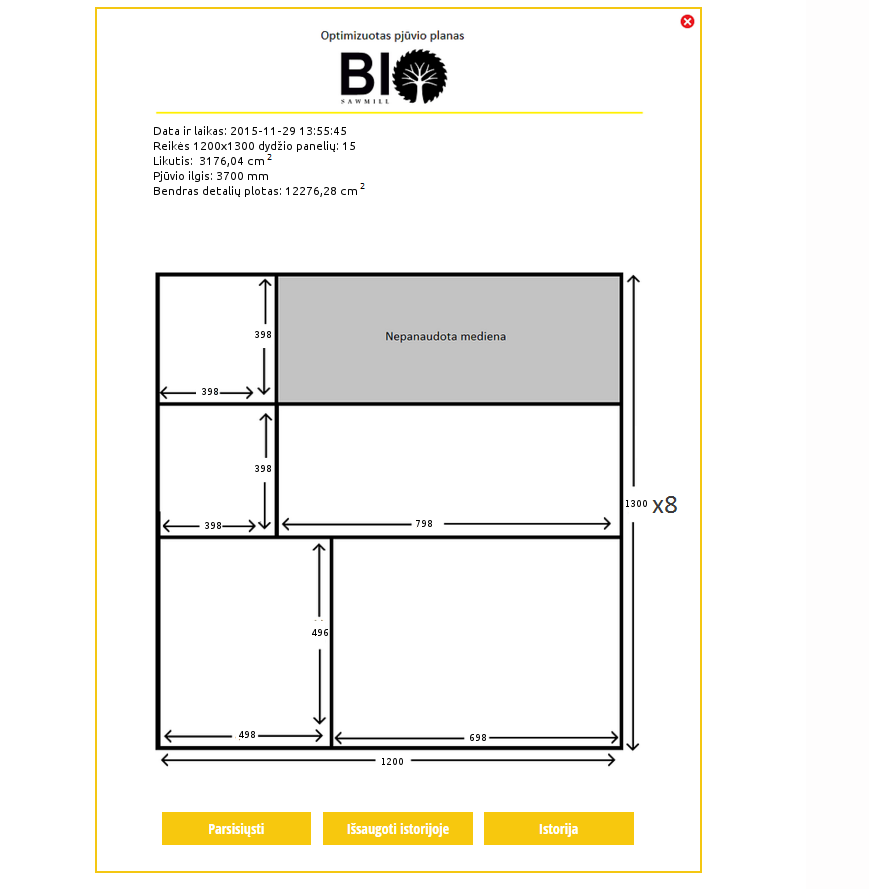
\includegraphics[scale=1.2]{interfeisai/optimizavimoPuslapisPrisijungusPasirinktoPerziura2}

\subsection{Optimizavimo puslapis - pasirinkto plano išsaugojimas}
\hspace{-2cm}
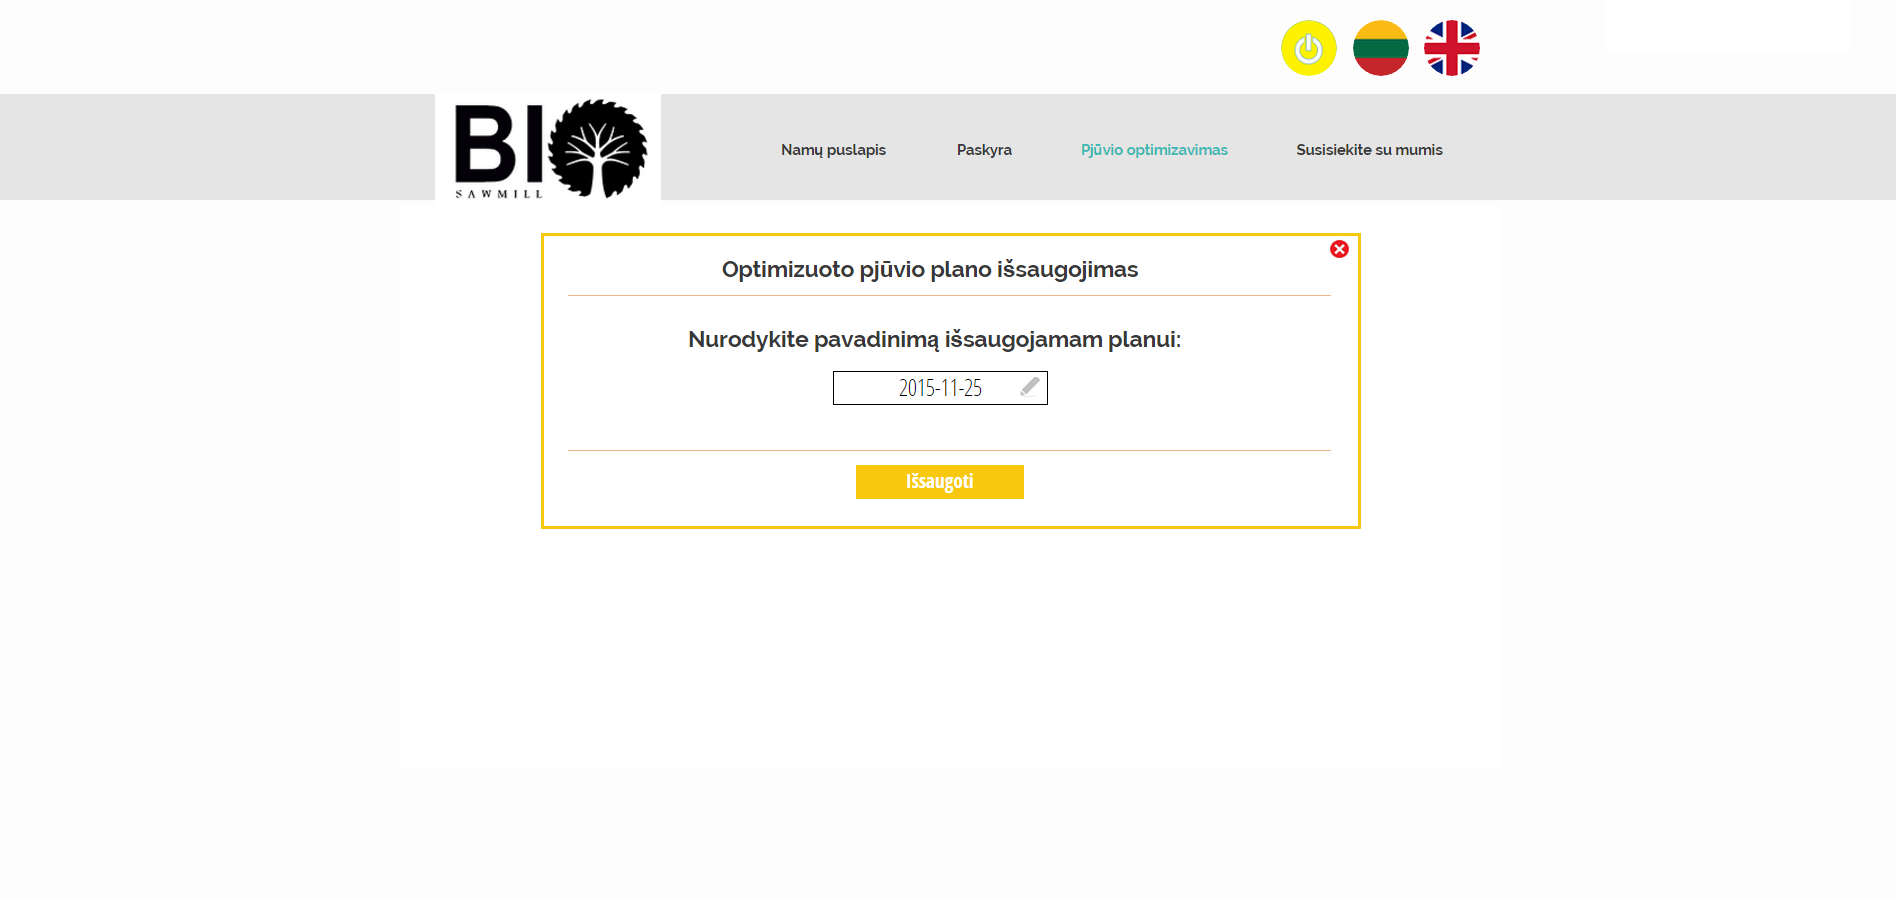
\includegraphics[scale=0.5]{interfeisai/optimizavimoPuslapisPrisijungusPasirinktoPlanoIsaugojimas}

\subsection{Optimizavimo puslapis - pasirinkto plano išsaugojimas (su klaida)}
\hspace{-2cm}
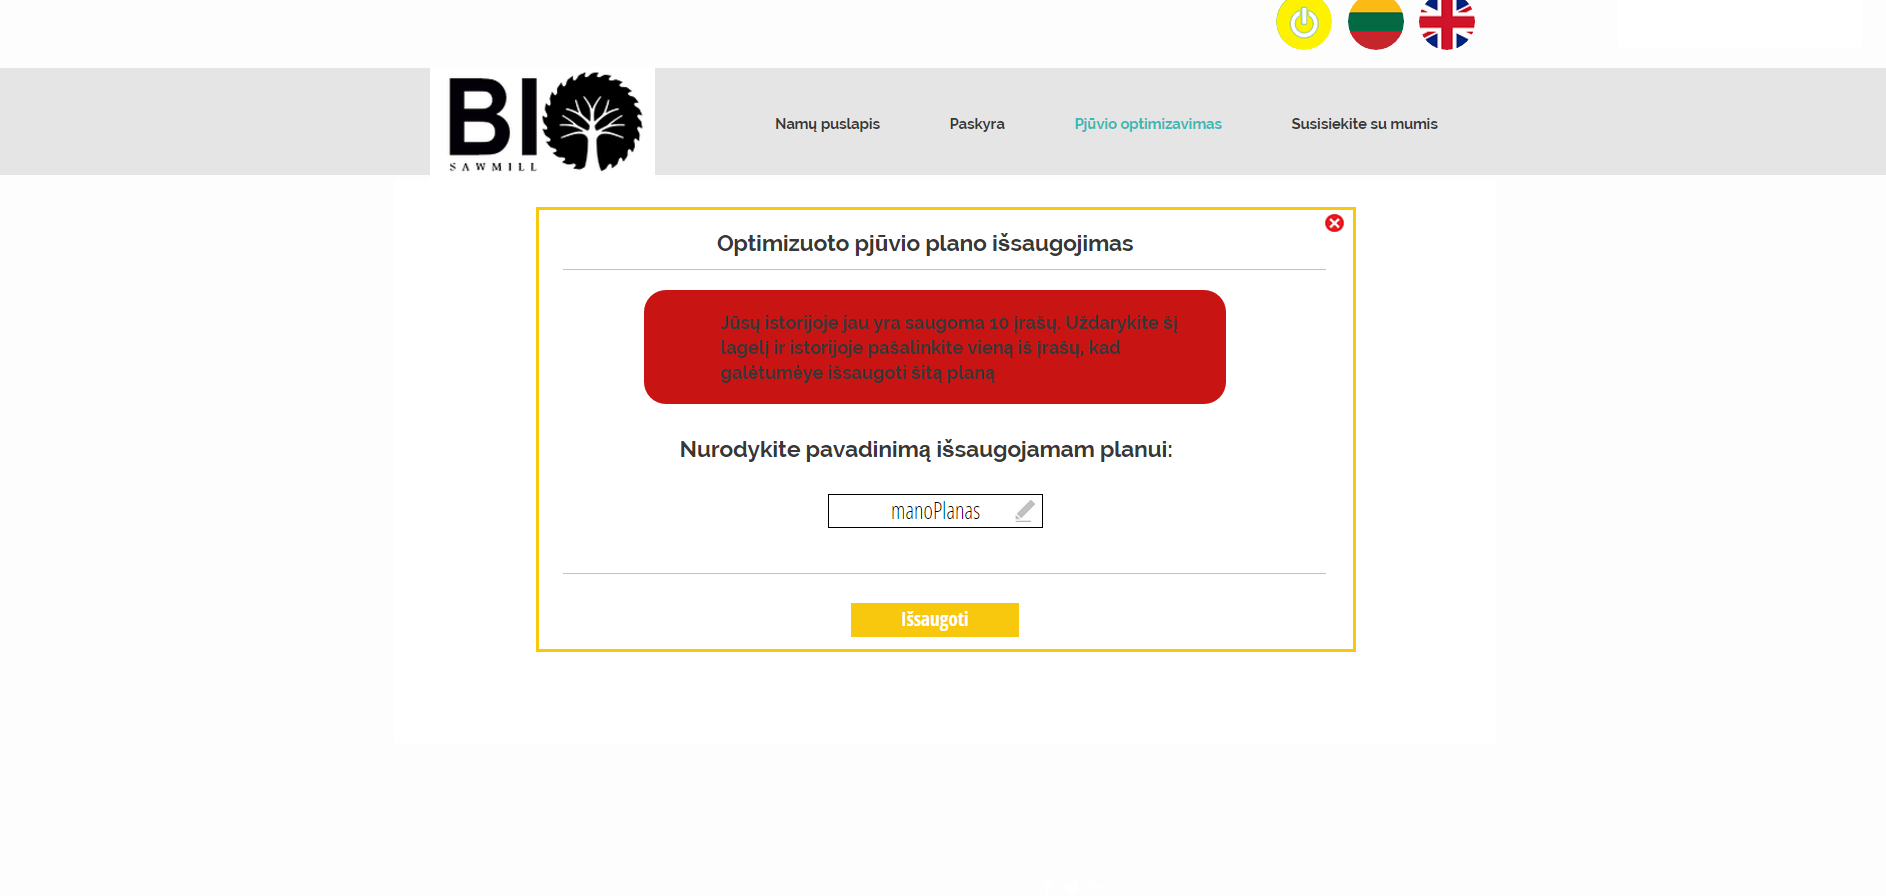
\includegraphics[scale=0.5]{interfeisai/optimizavimoPuslapisPrisijungusPasirinktoPlanoIsaugojimasSuKlaida}

\subsection{Optimizavimo puslapis - istorijos peržiūra}
\hspace{-2cm}
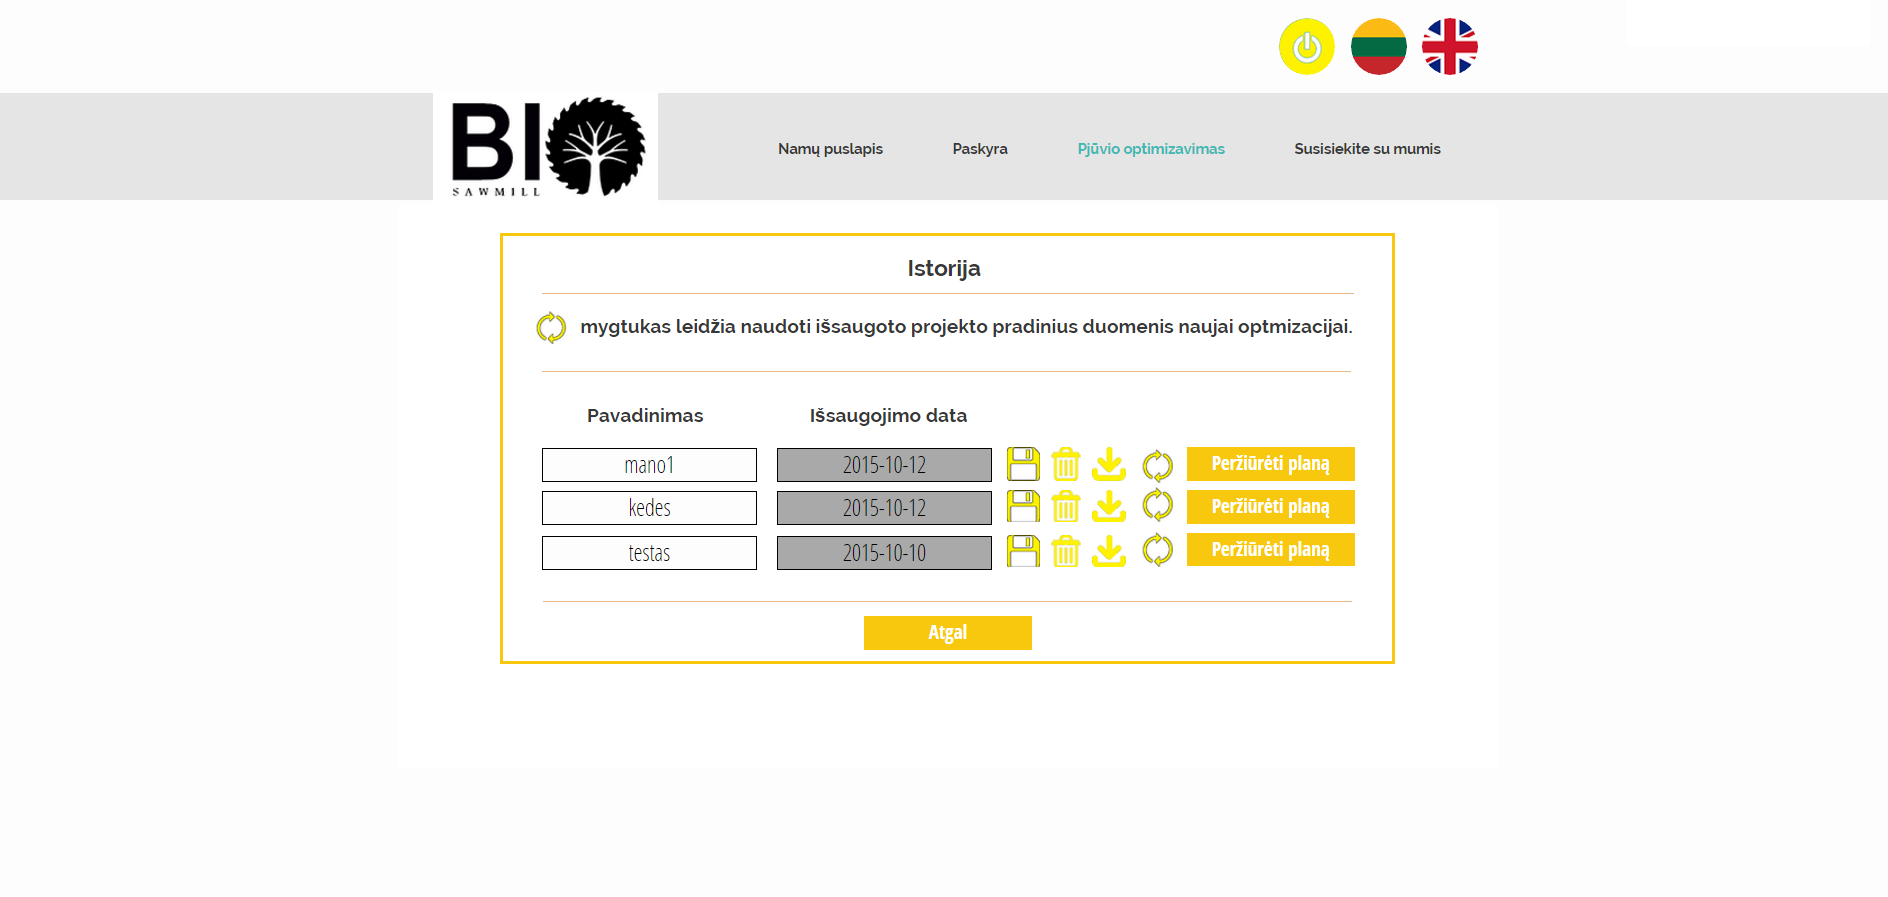
\includegraphics[scale=0.5]{interfeisai/optimizavimoPuslapisPrisijungusIstorija}

\subsection{Optimizavimo puslapis - istorijos redagavimas (su klaida)}
\hspace{-2cm}
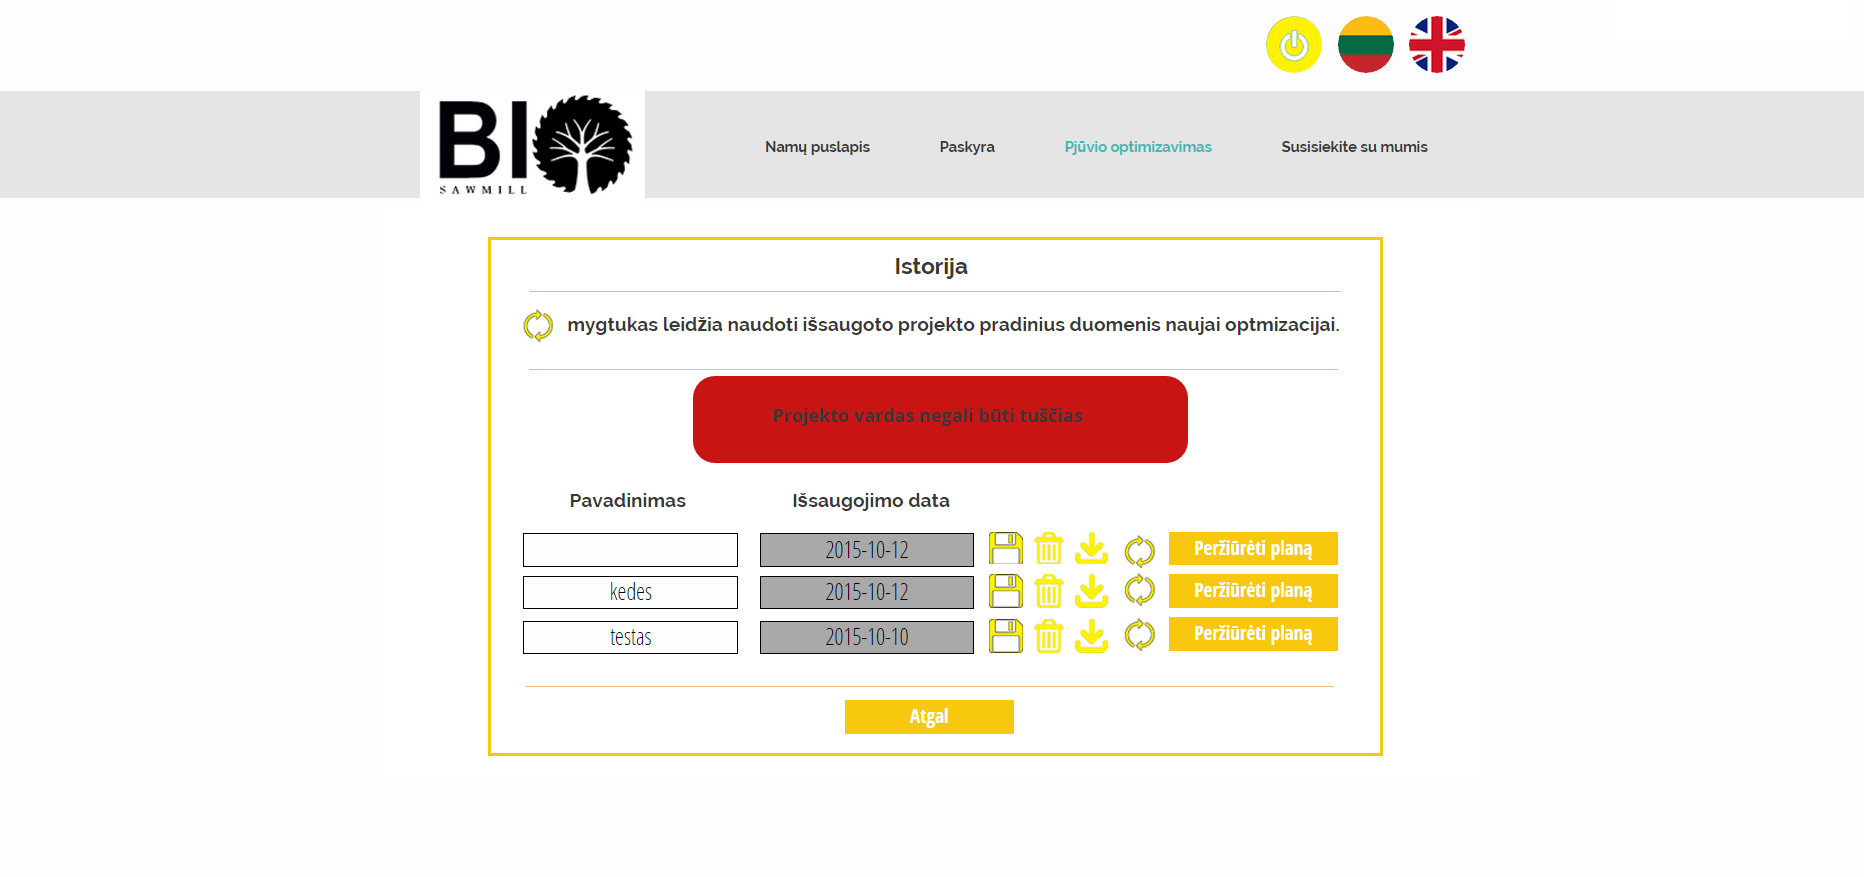
\includegraphics[scale=0.5]{interfeisai/optimizavimoPuslapisPrisijungusIstorijaSuKlaida}

\subsection{Optimizavimo puslapis - išsaugoto plano istorijoje peržiūra (iš arčiau)}
\hspace{-2cm}
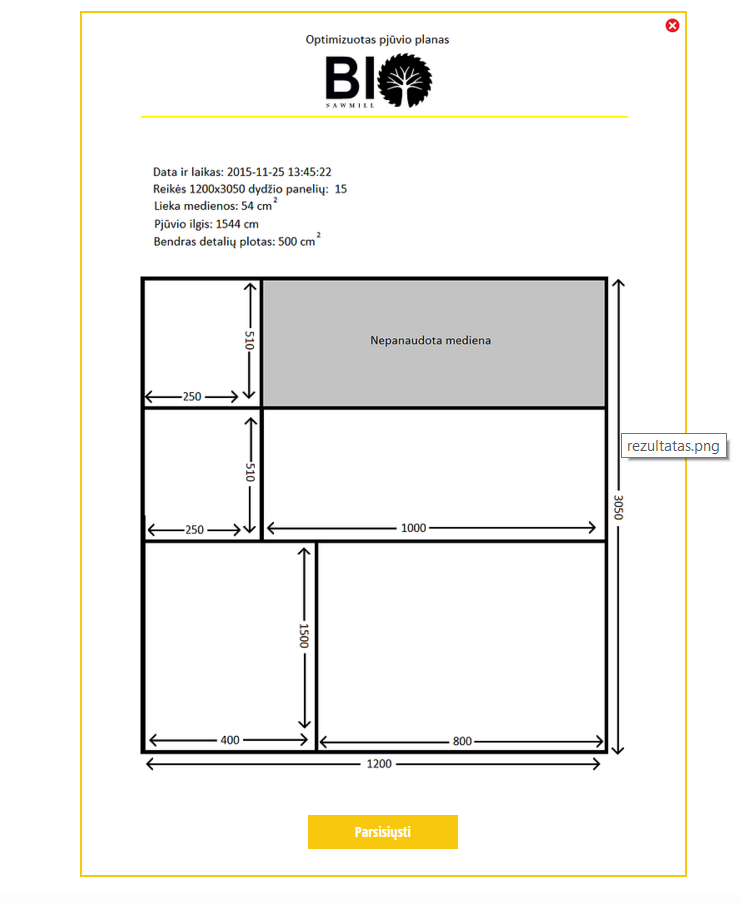
\includegraphics[scale=1.2]{interfeisai/optimizavimoPuslapisPrisijungusIsaugotasPlanas}

\subsection{Susisiekimo su mumis puslapis}
\hspace{-2cm}
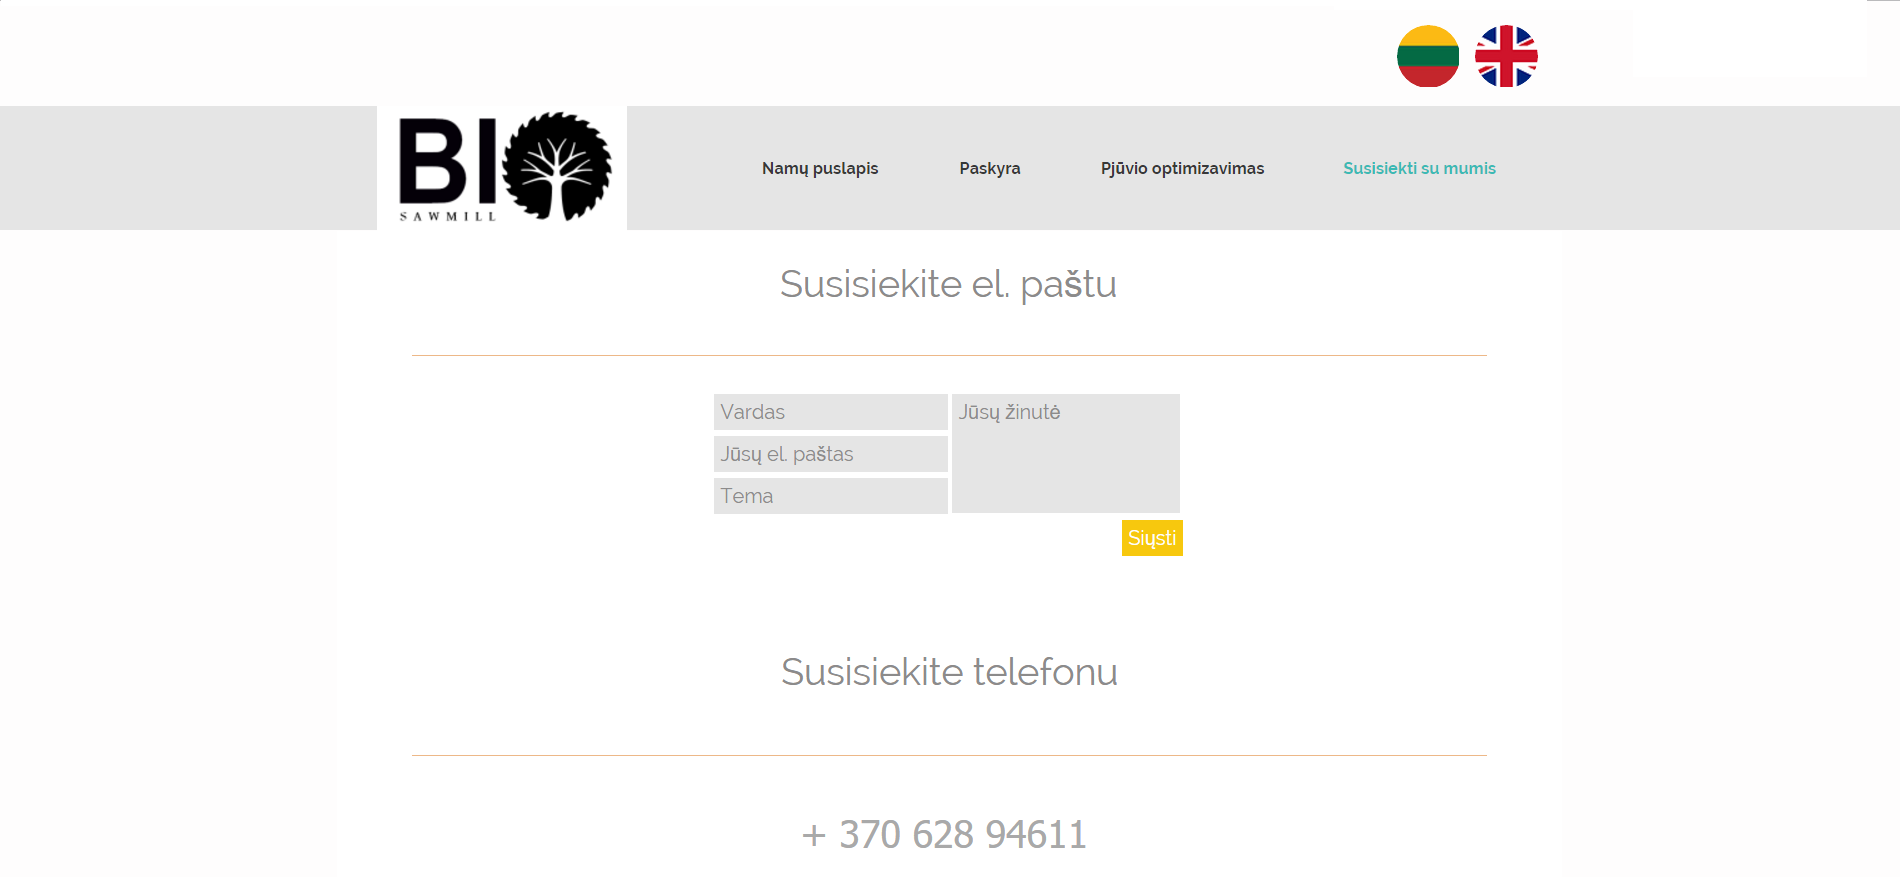
\includegraphics[scale=0.5]{interfeisai/susisiekimas}

\subsection{Susisiekimo su mumis puslapis (su klaida)}
\hspace{-2cm}
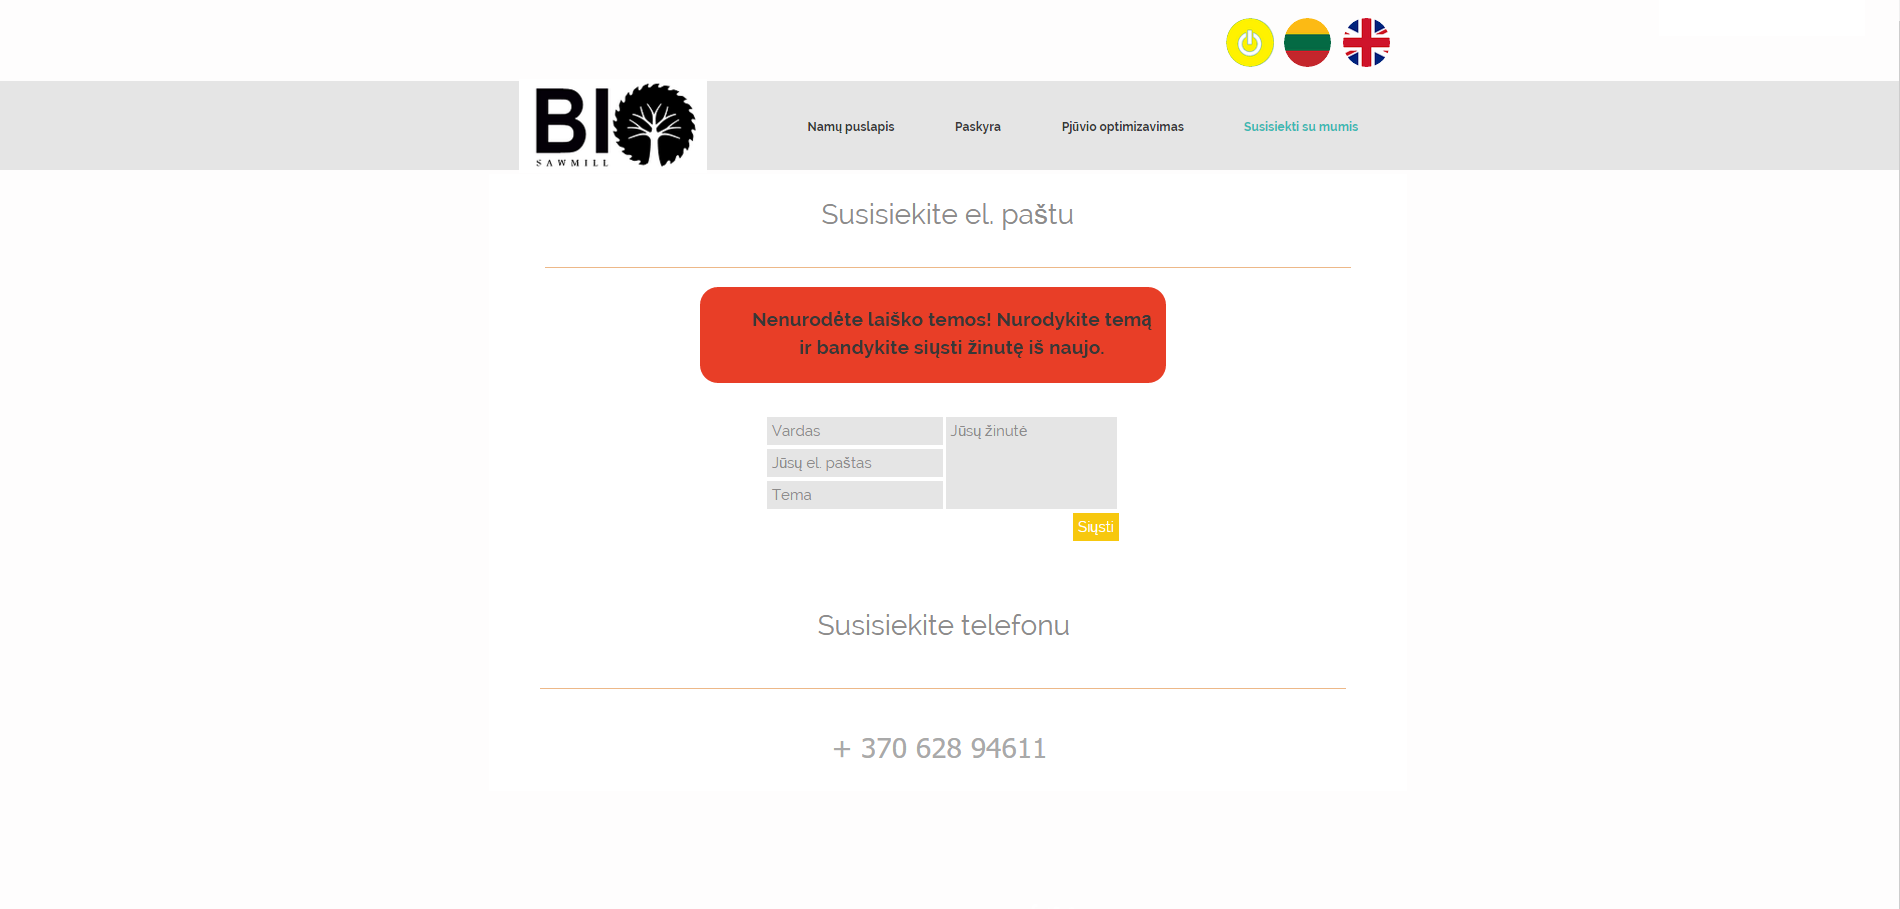
\includegraphics[scale=0.5]{interfeisai/susisiekimasSuKlaida}

% ---------------------------------- UZKOMENTUOTA, NEISTRINTI  ------------------------------
\begin{comment}
\subsection{Namų puslapis (vartotojas prisijungęs)}
\hspace{-2cm}
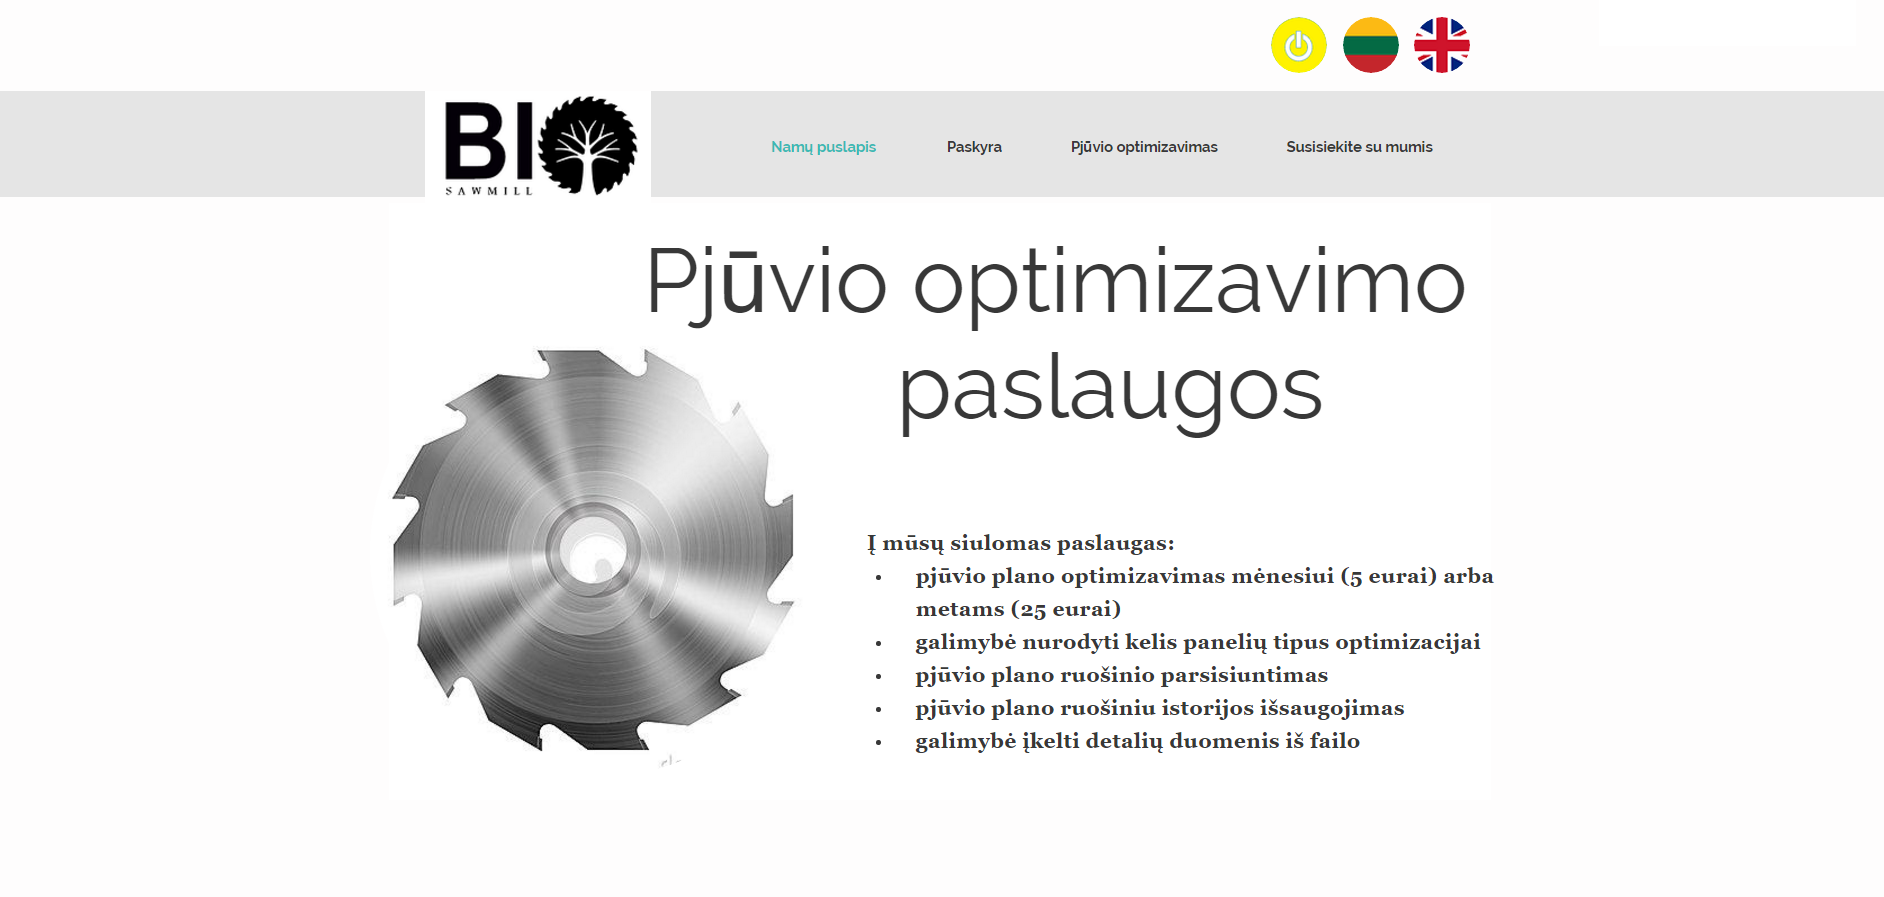
\includegraphics[scale=0.5]{interfeisai/pagrindinis}

\subsection{Vartotojo paskyros puslapis - vartotojas neprisijungęs}
\hspace{-2cm}
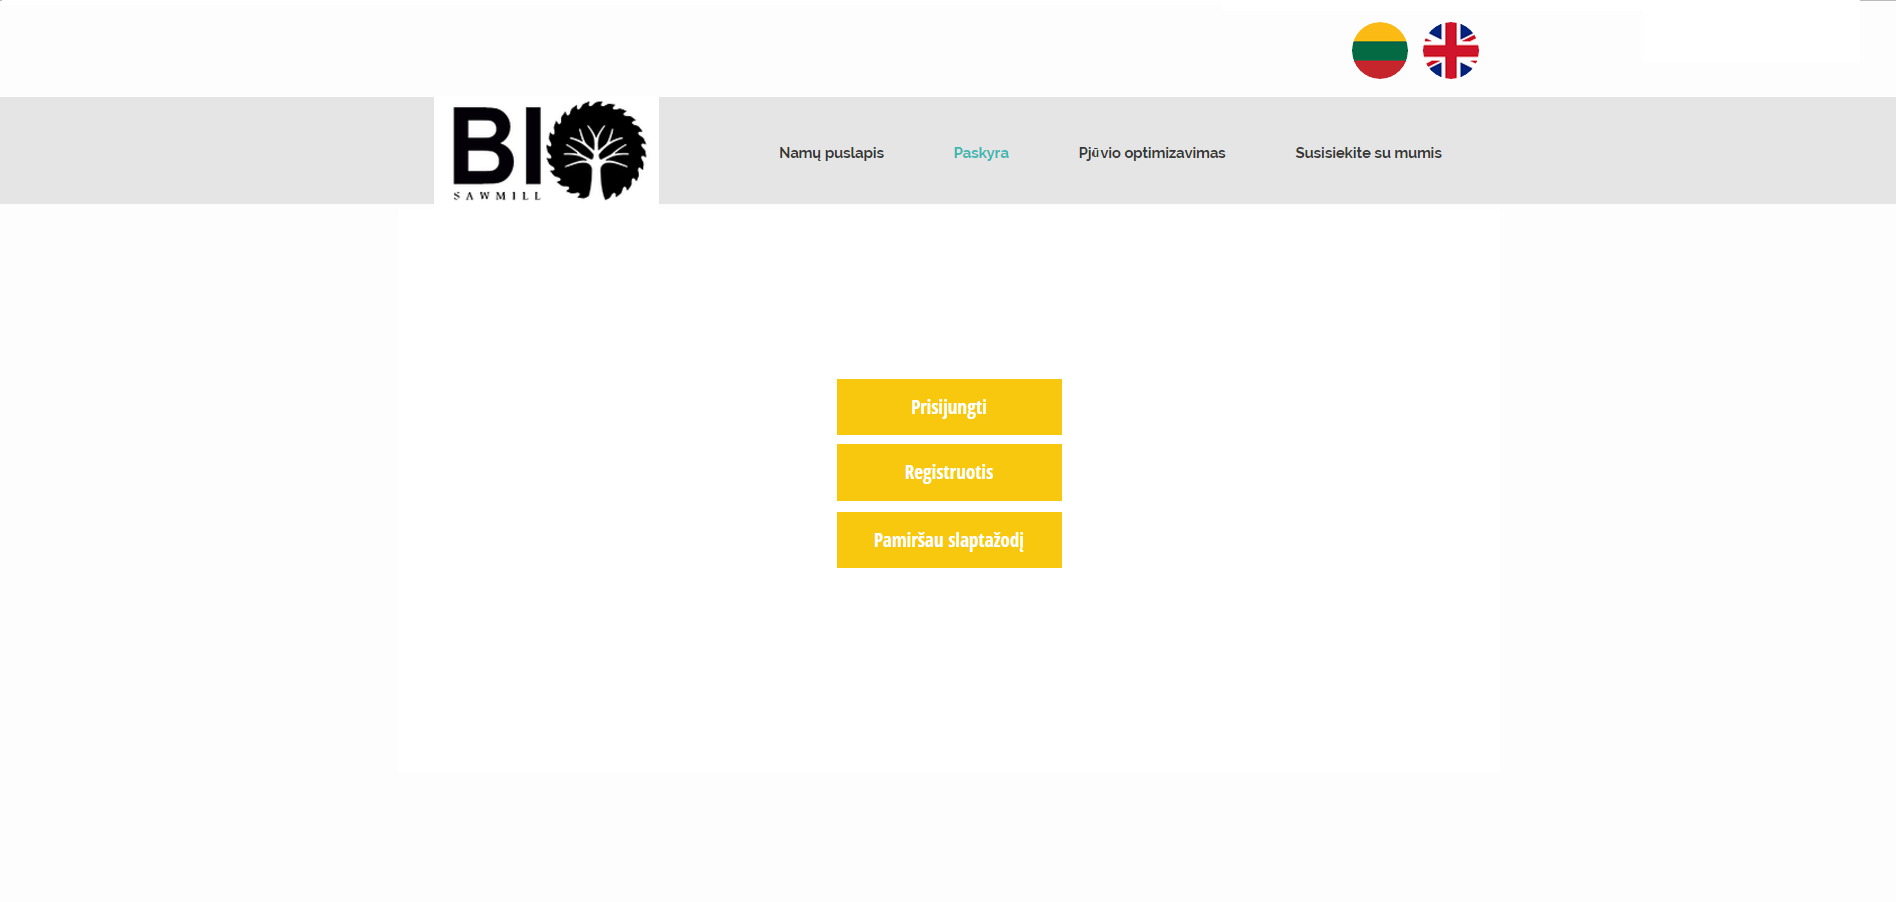
\includegraphics[scale=0.5]{interfeisai/paskyrosPuslapisNeprisijungta}

\subsection{Vartotojo paskyros puslapis - registracija}
\hspace{-2cm}
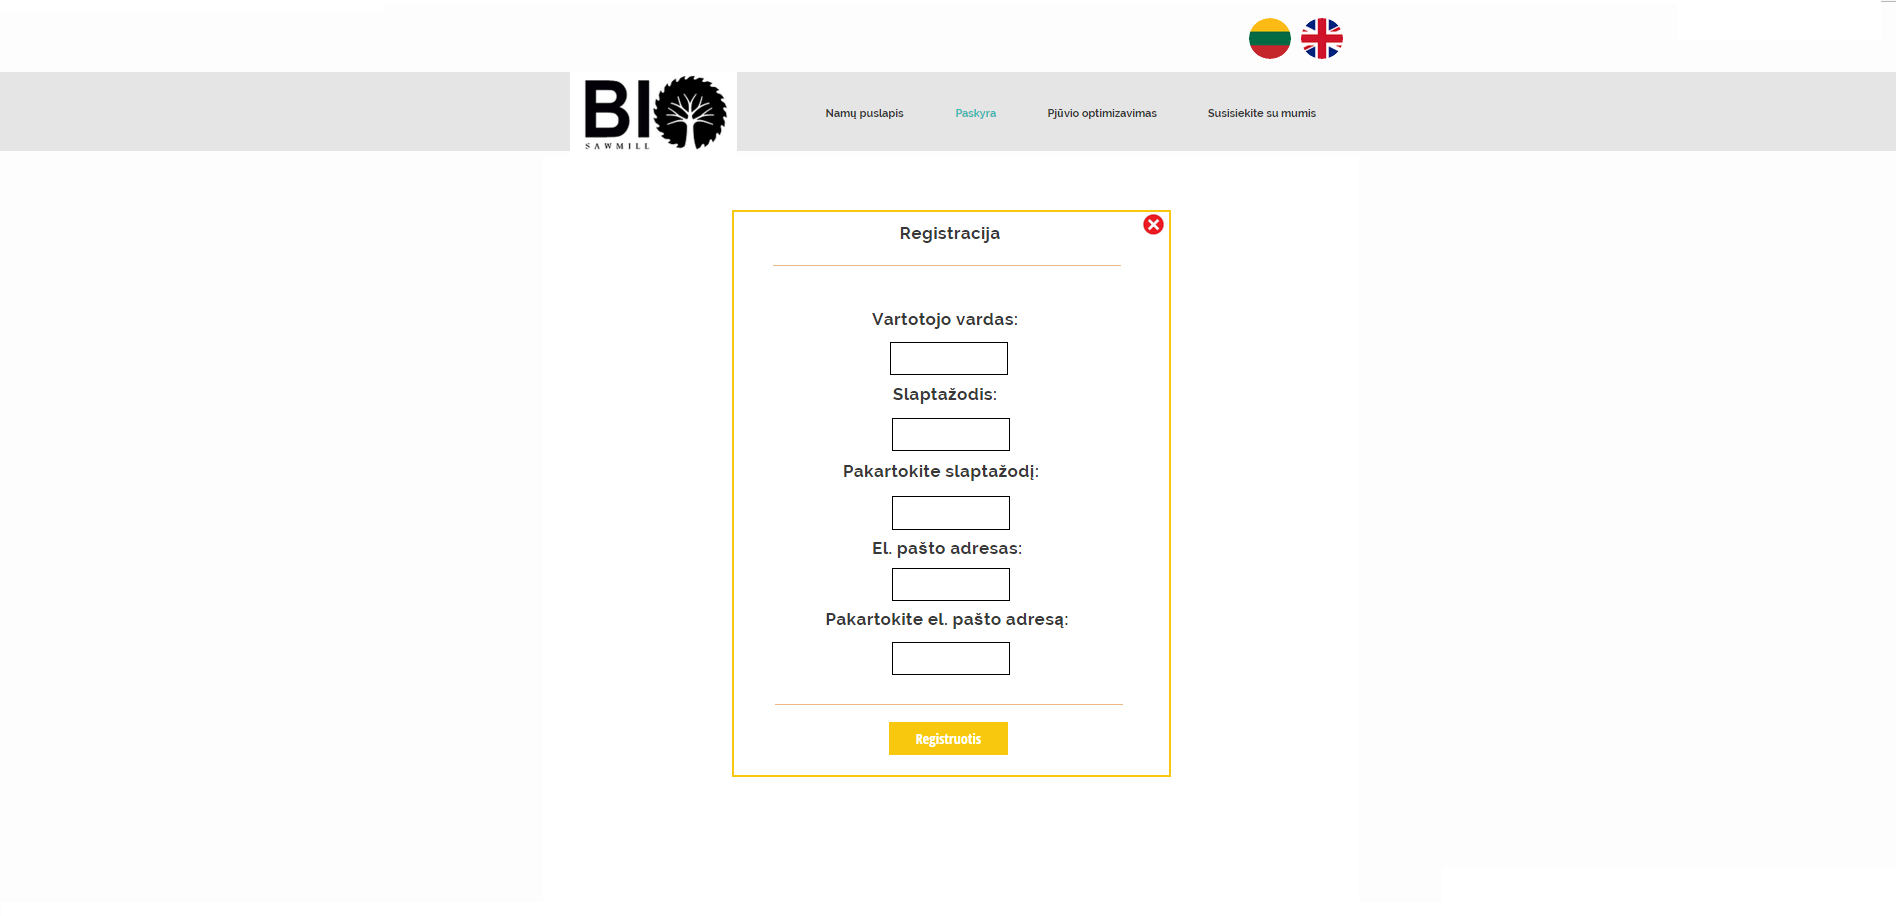
\includegraphics[scale=0.5]{interfeisai/paskyrosPuslapisRegistracija}

\subsection{Vartotojo paskyros puslapis - registracija (su klaida)}
\hspace{-2cm}
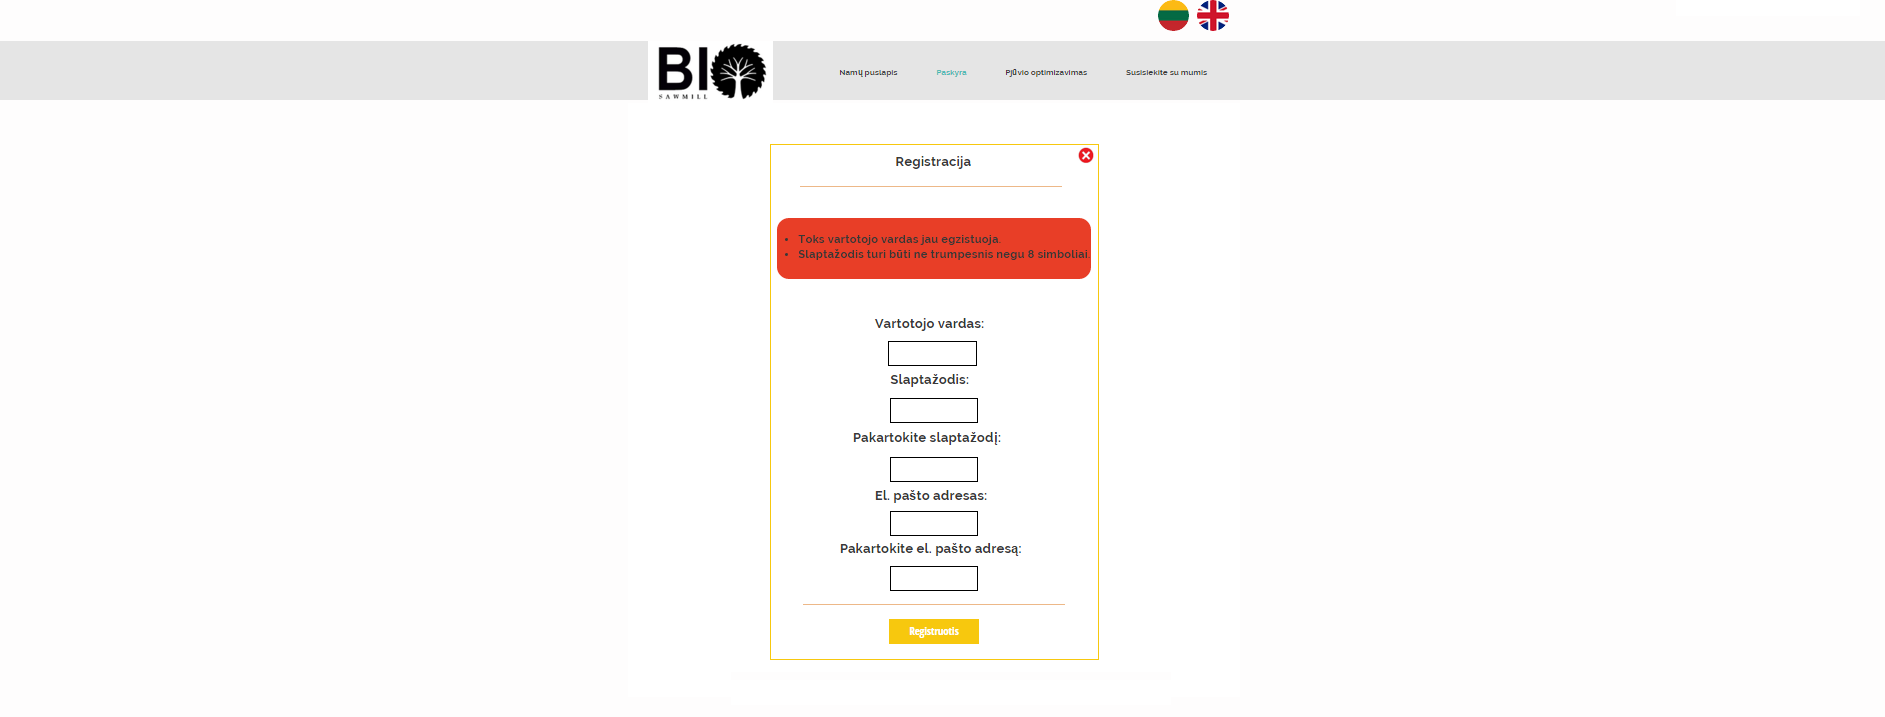
\includegraphics[scale=0.5]{interfeisai/paskyrosPuslapisRegistracijaSuKlaida}

\subsection{Vartotojo paskyros puslapis - sėkminga registracija}
\hspace{-2cm}
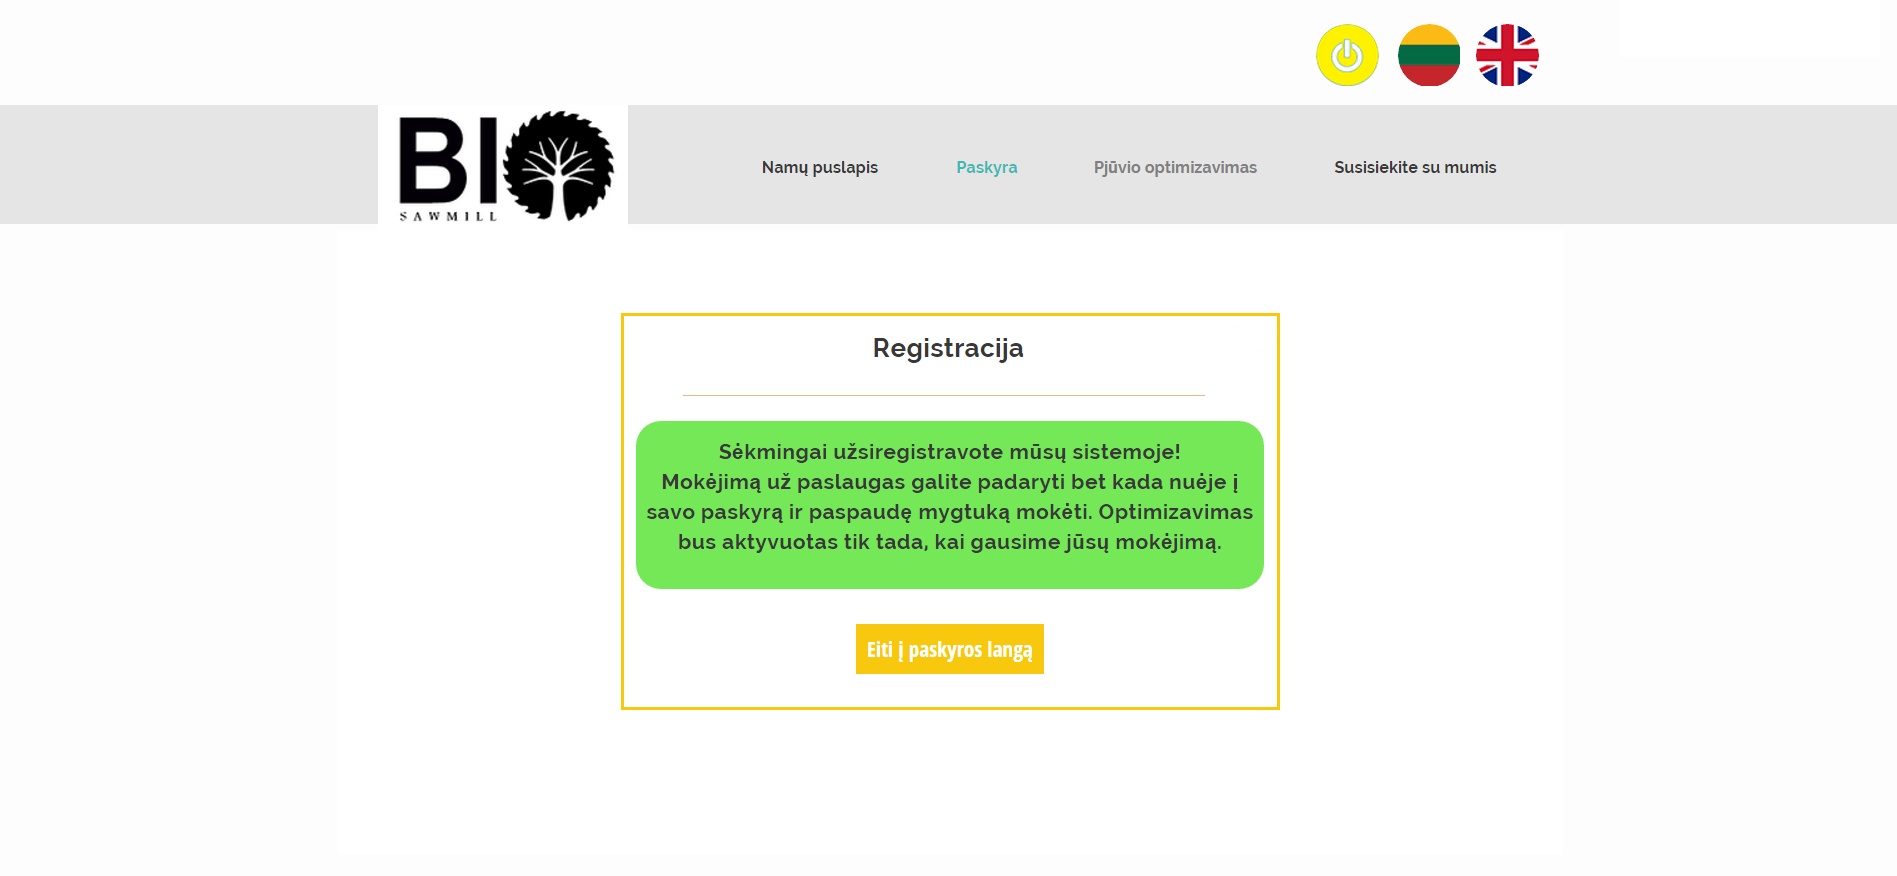
\includegraphics[scale=0.5]{interfeisai/paskyrosPuslapisRegistracijaSekminga}

\subsection{Vartotojo paskyros puslapis - prisijungimas}
\hspace{-2cm}
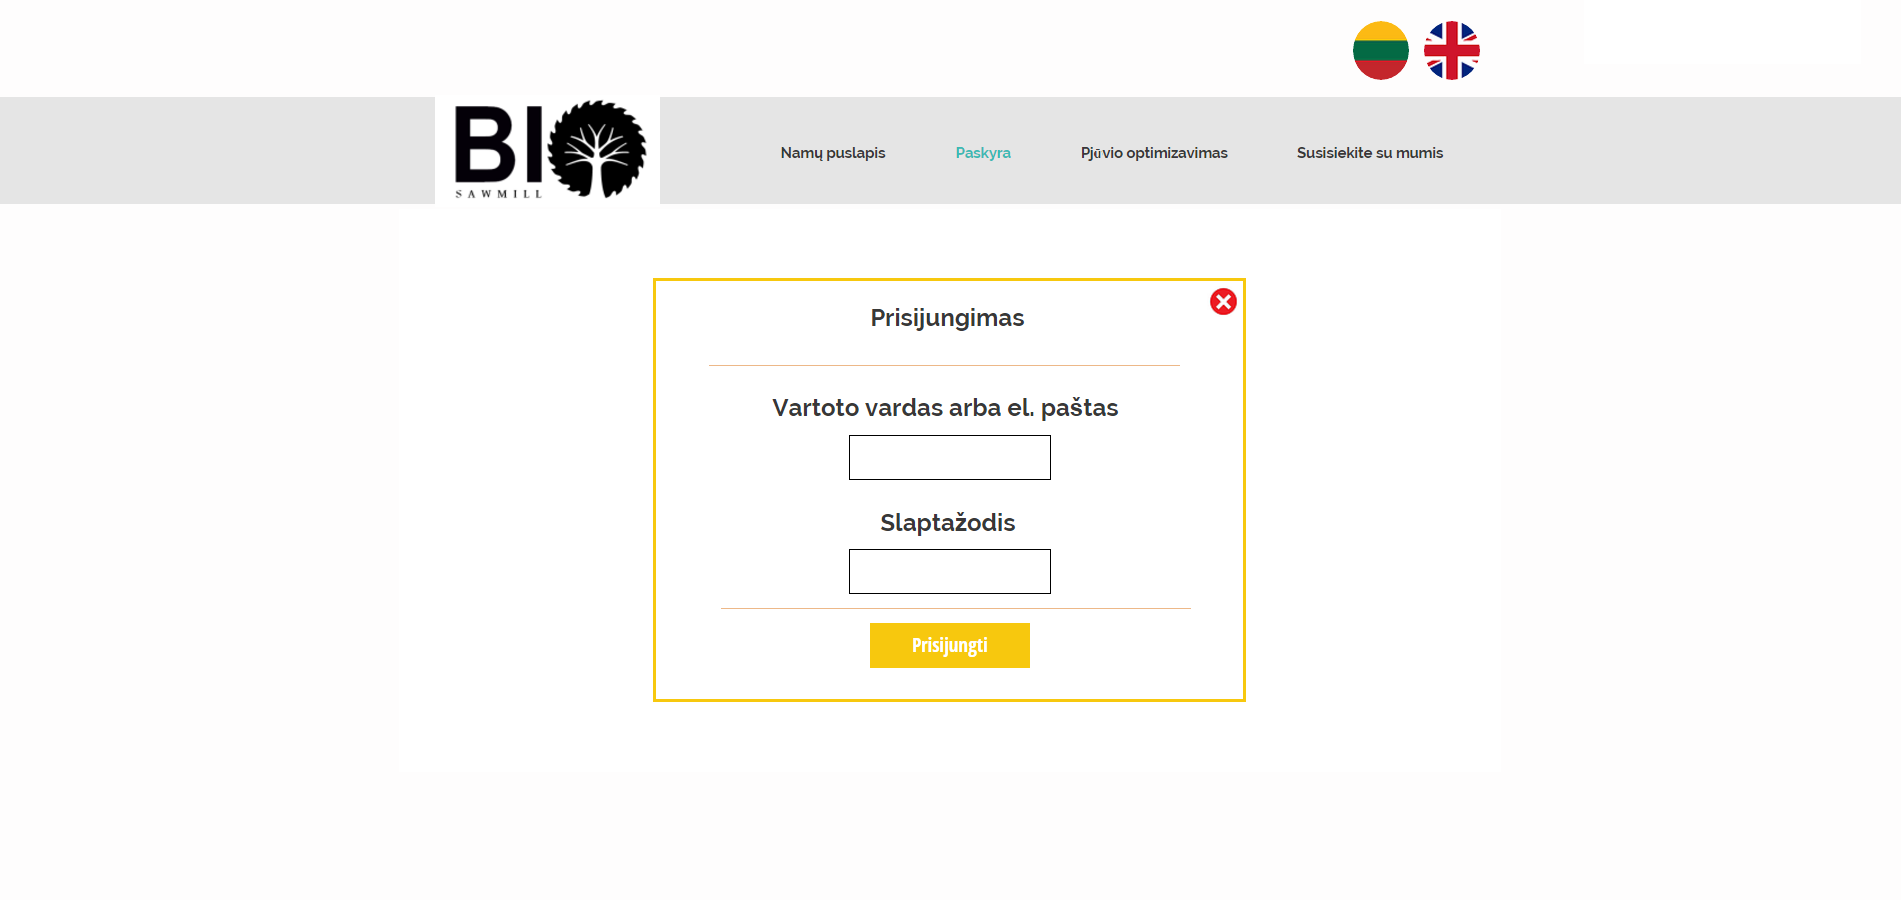
\includegraphics[scale=0.5]{interfeisai/paskyrosPuslapisPrisijungimas}

\subsection{Vartotojo paskyros puslapis - prisijungimas (su klaida)}
\hspace{-2cm}
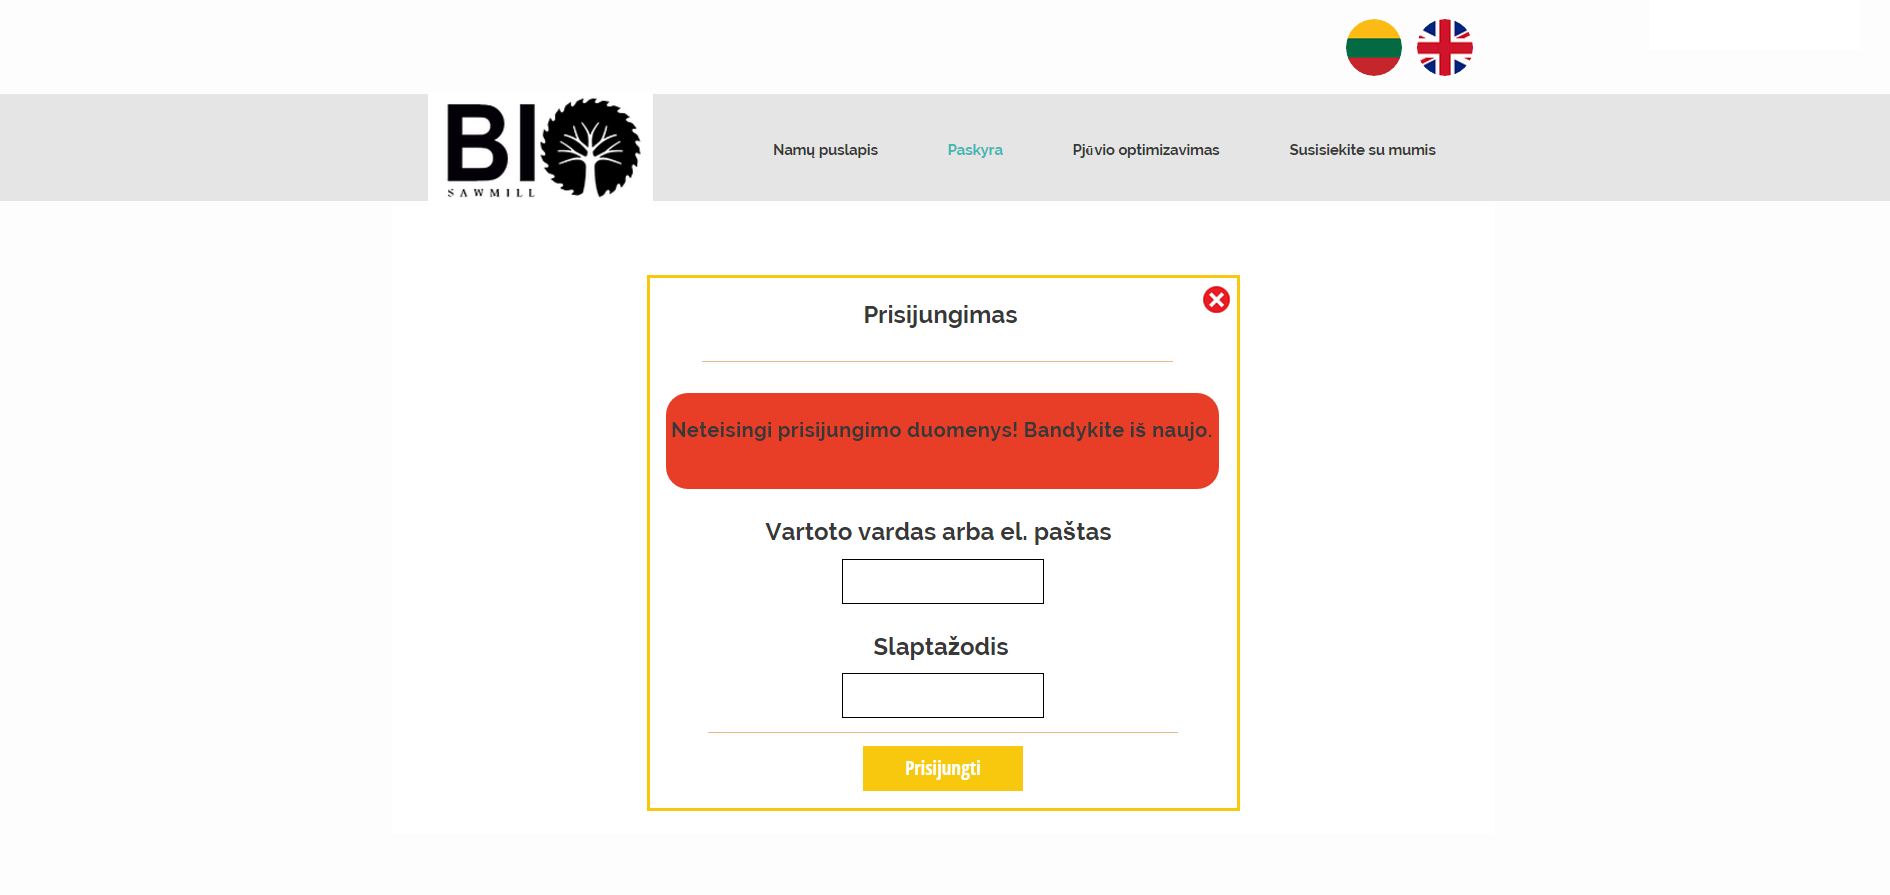
\includegraphics[scale=0.5]{interfeisai/paskyrosPuslapisPrisijungimasSuKlaida}

\subsection{Vartotojo paskyros puslapis - pamirštas slaptažodis}
\hspace{-2cm}
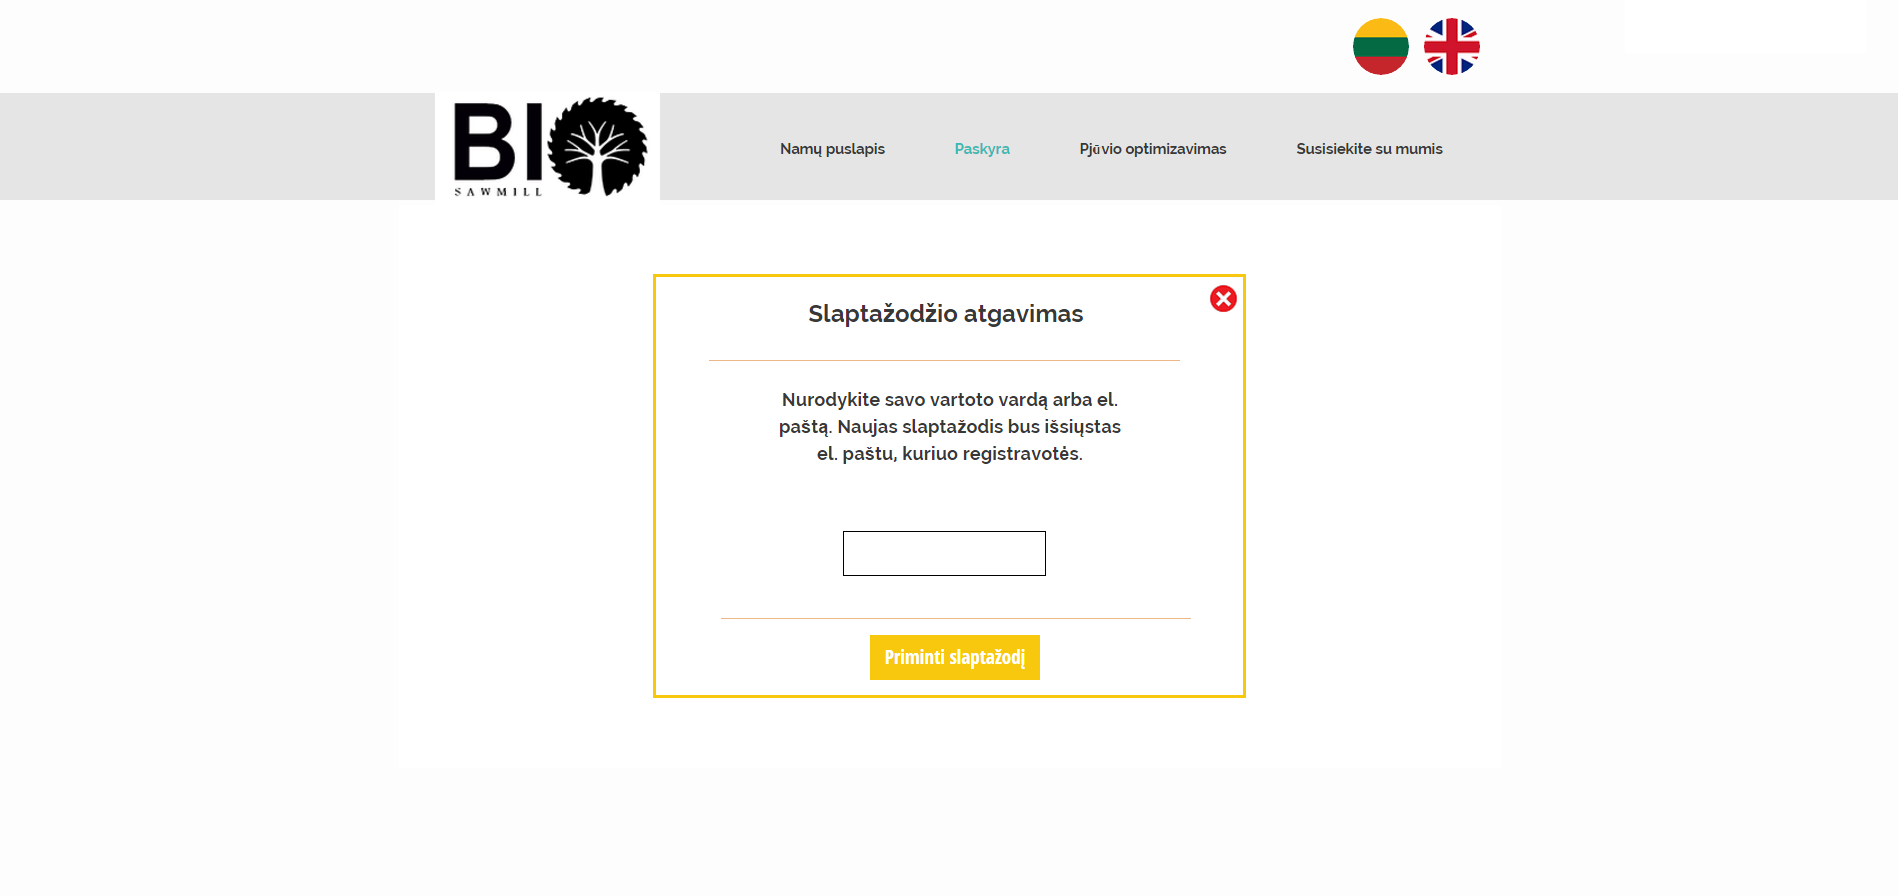
\includegraphics[scale=0.5]{interfeisai/paskyrosPuslapisPamirstasSlaptazodis}

\subsection{Vartotojo paskyros puslapis - pamirštas slaptažodis 2}
\hspace{-2cm}
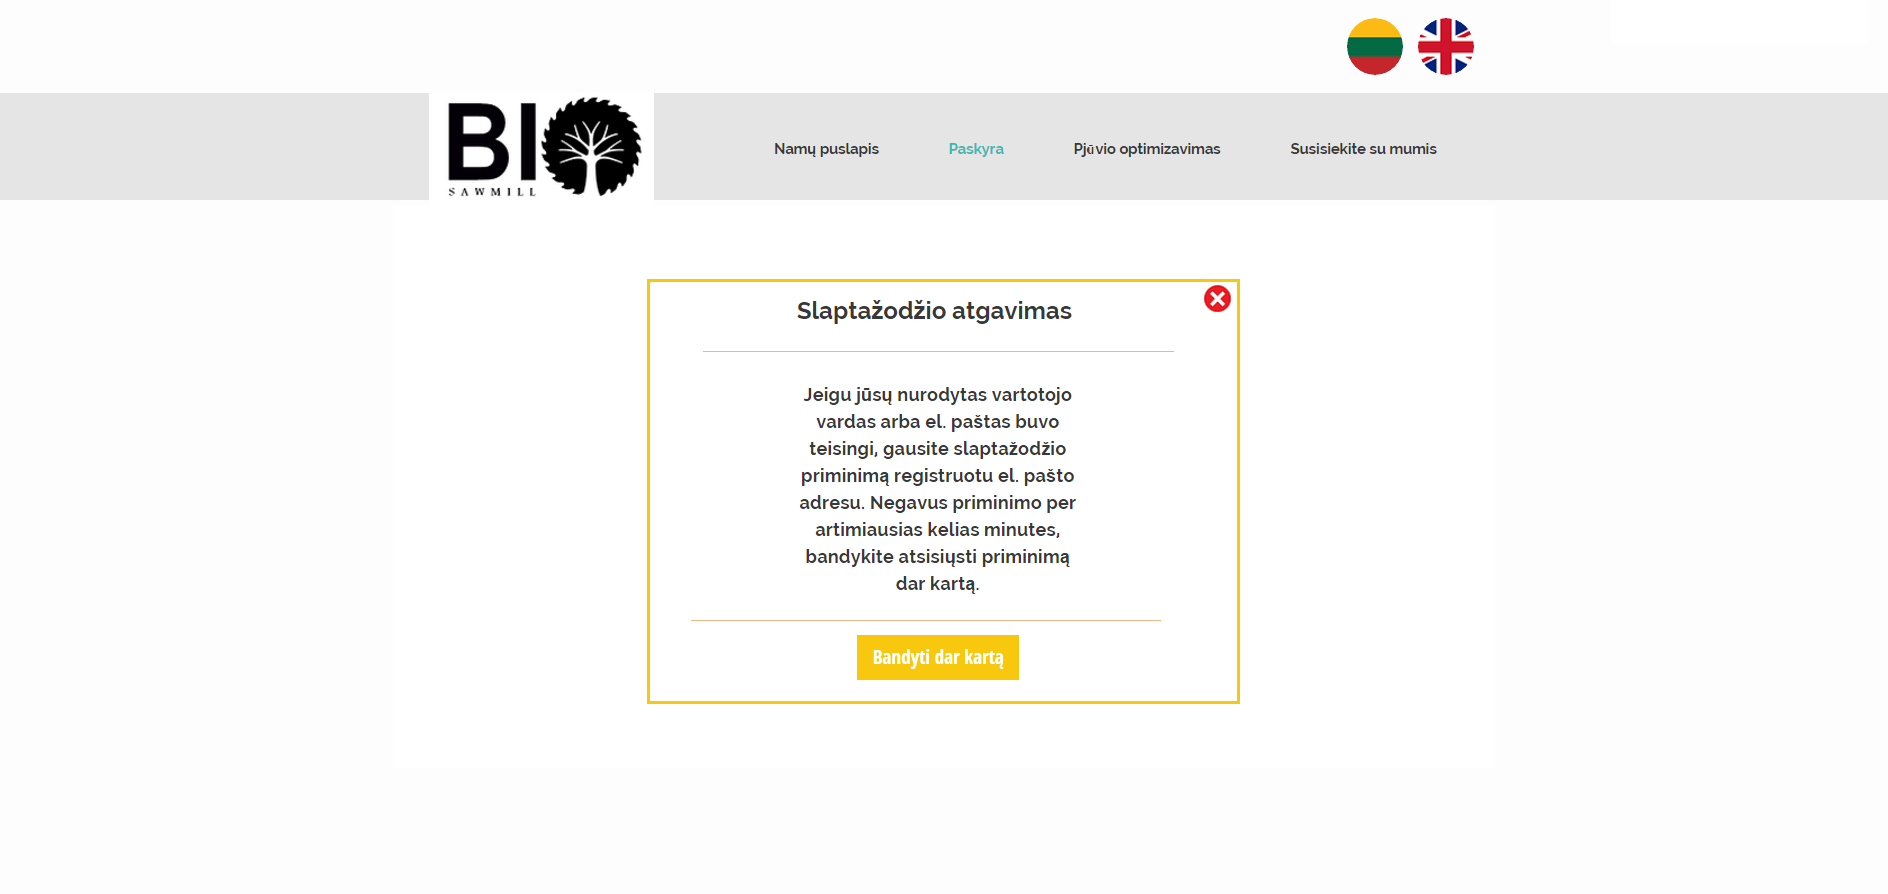
\includegraphics[scale=0.5]{interfeisai/paskyrosPuslapisPamirstasSlaptazodis2}

\subsection{Vartotojo paskyros puslapis - prisijungus (neapmokėta už paslaugas)}
\hspace{-2cm}
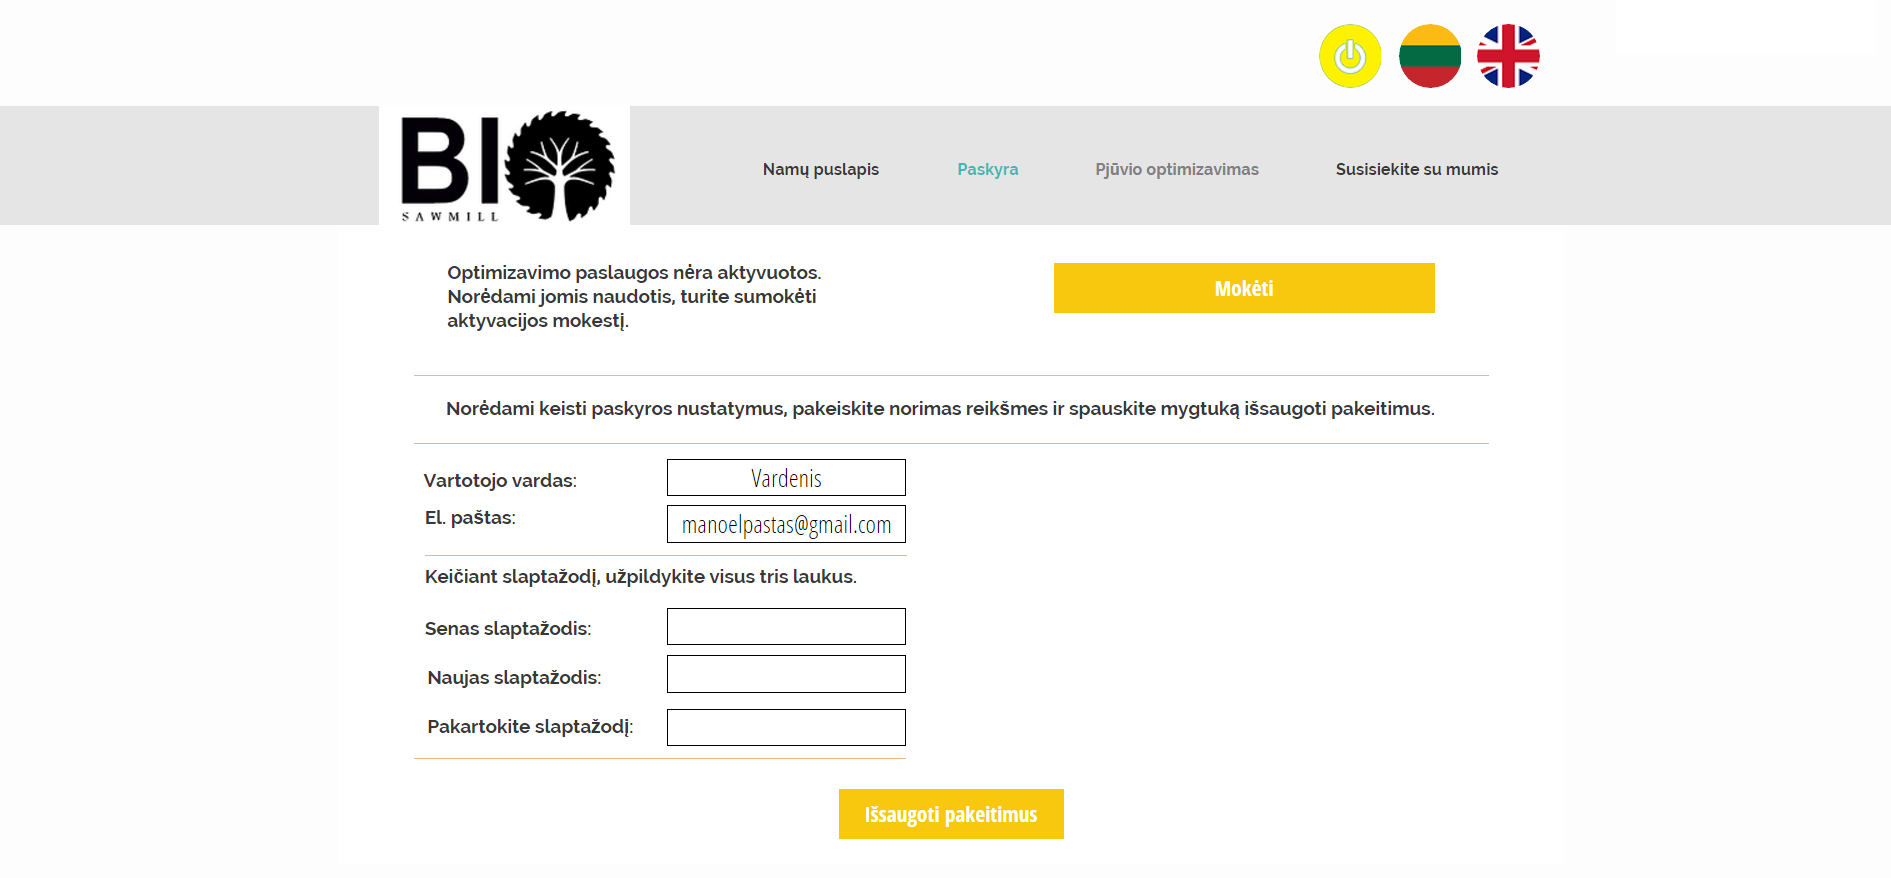
\includegraphics[scale=0.5]{interfeisai/paskyrosPuslapisVartotojasNeapmoketas}

\subsection{Vartotojo paskyros puslapis - prisijungus (apmokėta už paslaugas)}
\hspace{-2cm}
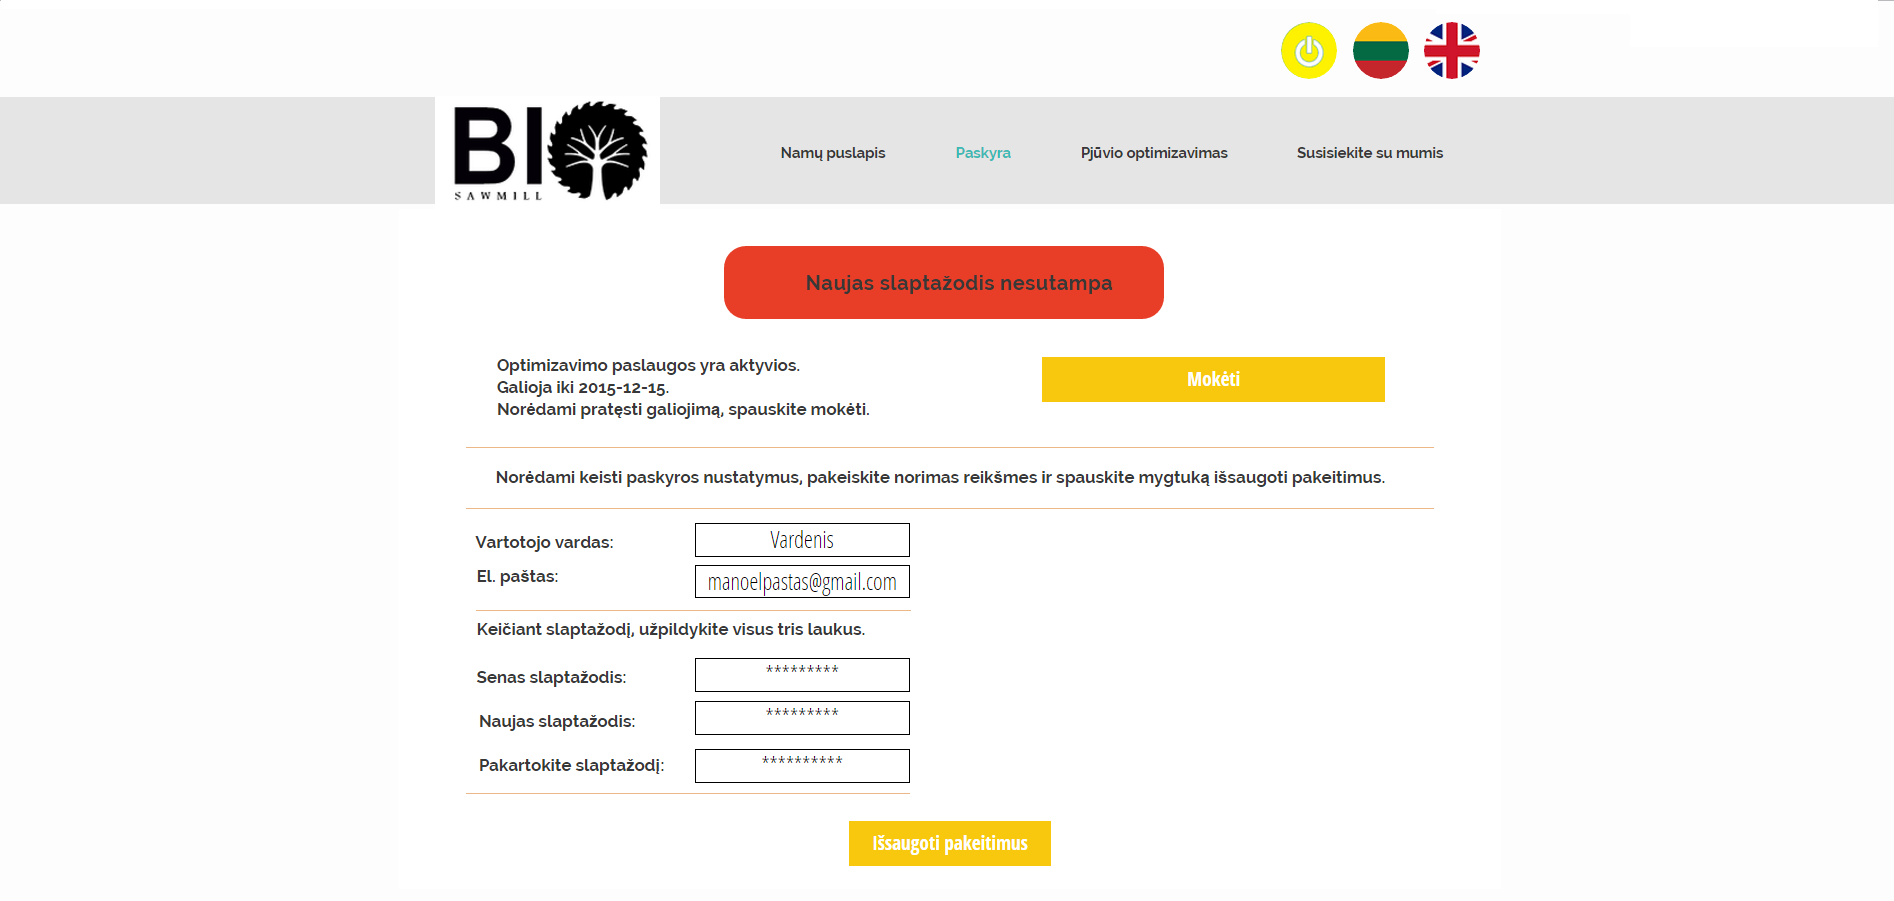
\includegraphics[scale=0.5]{interfeisai/paskyrosPuslapisVartotojasApmoketas}

\subsection{Vartotojo paskyros puslapis - prisijungus - mokėjimas}
\hspace{-2cm}
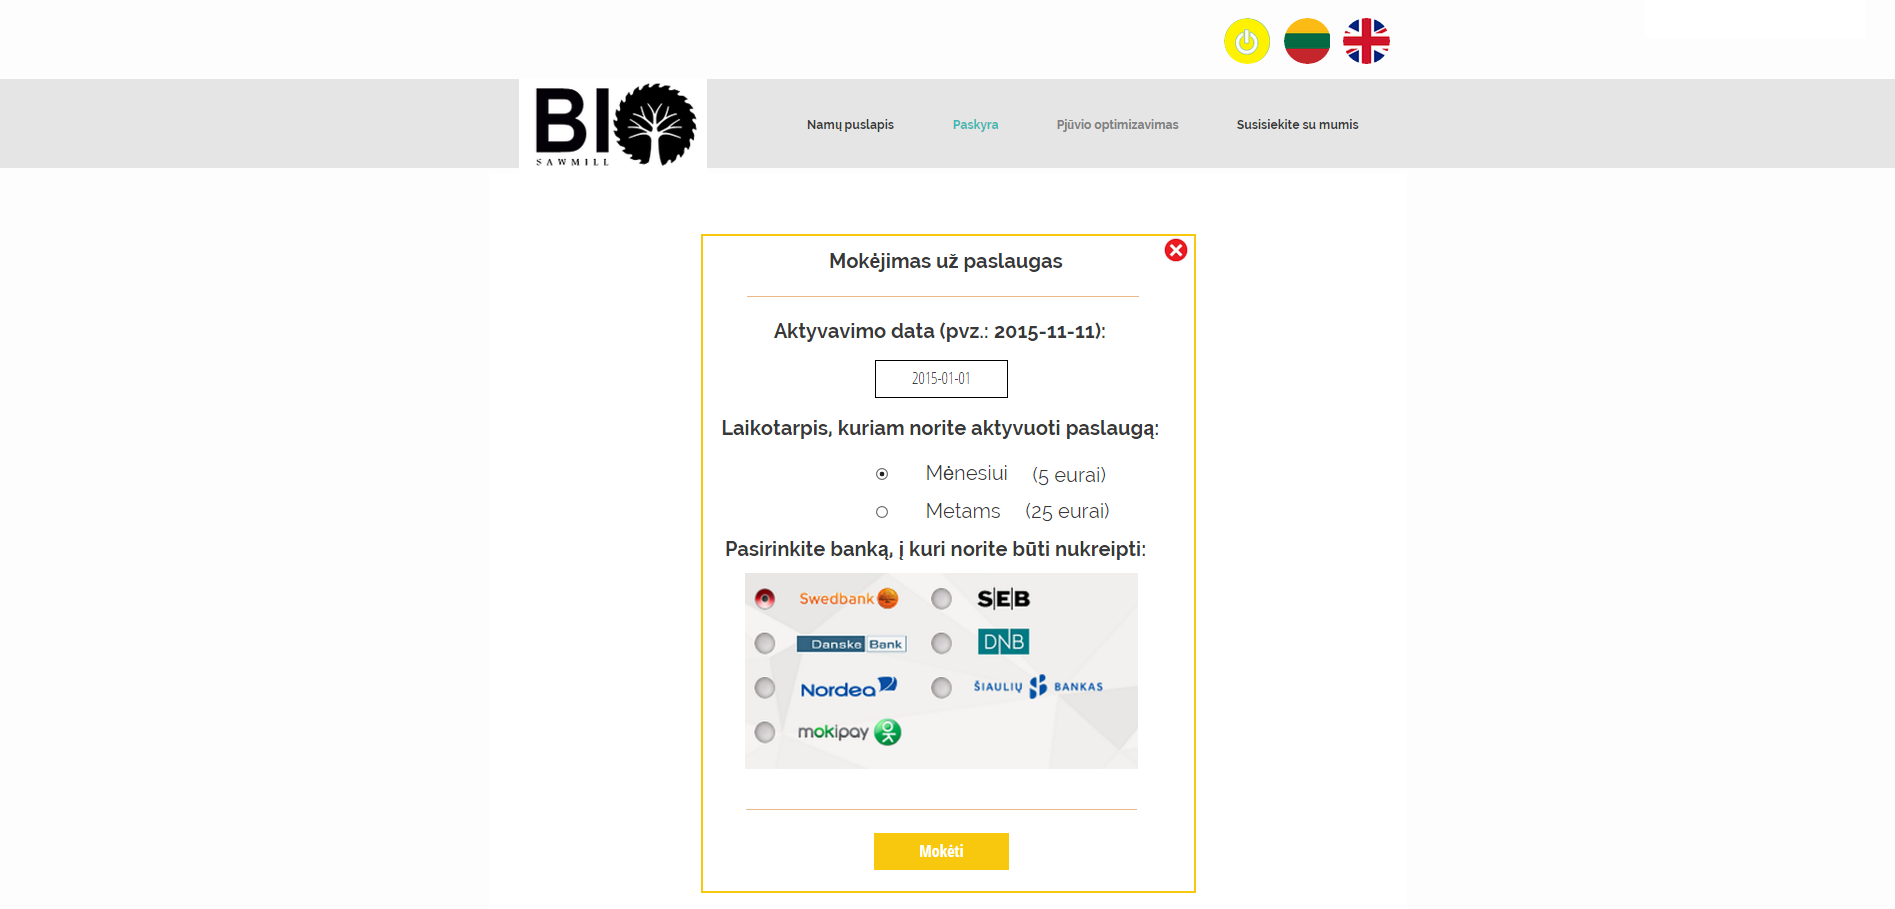
\includegraphics[scale=0.5]{interfeisai/paskyrosPuslapisVartotojasMokejimas}

\subsection{Vartotojo paskyros puslapis - prisijungus - mokėjimas (su klaida)}
\hspace{-2cm}
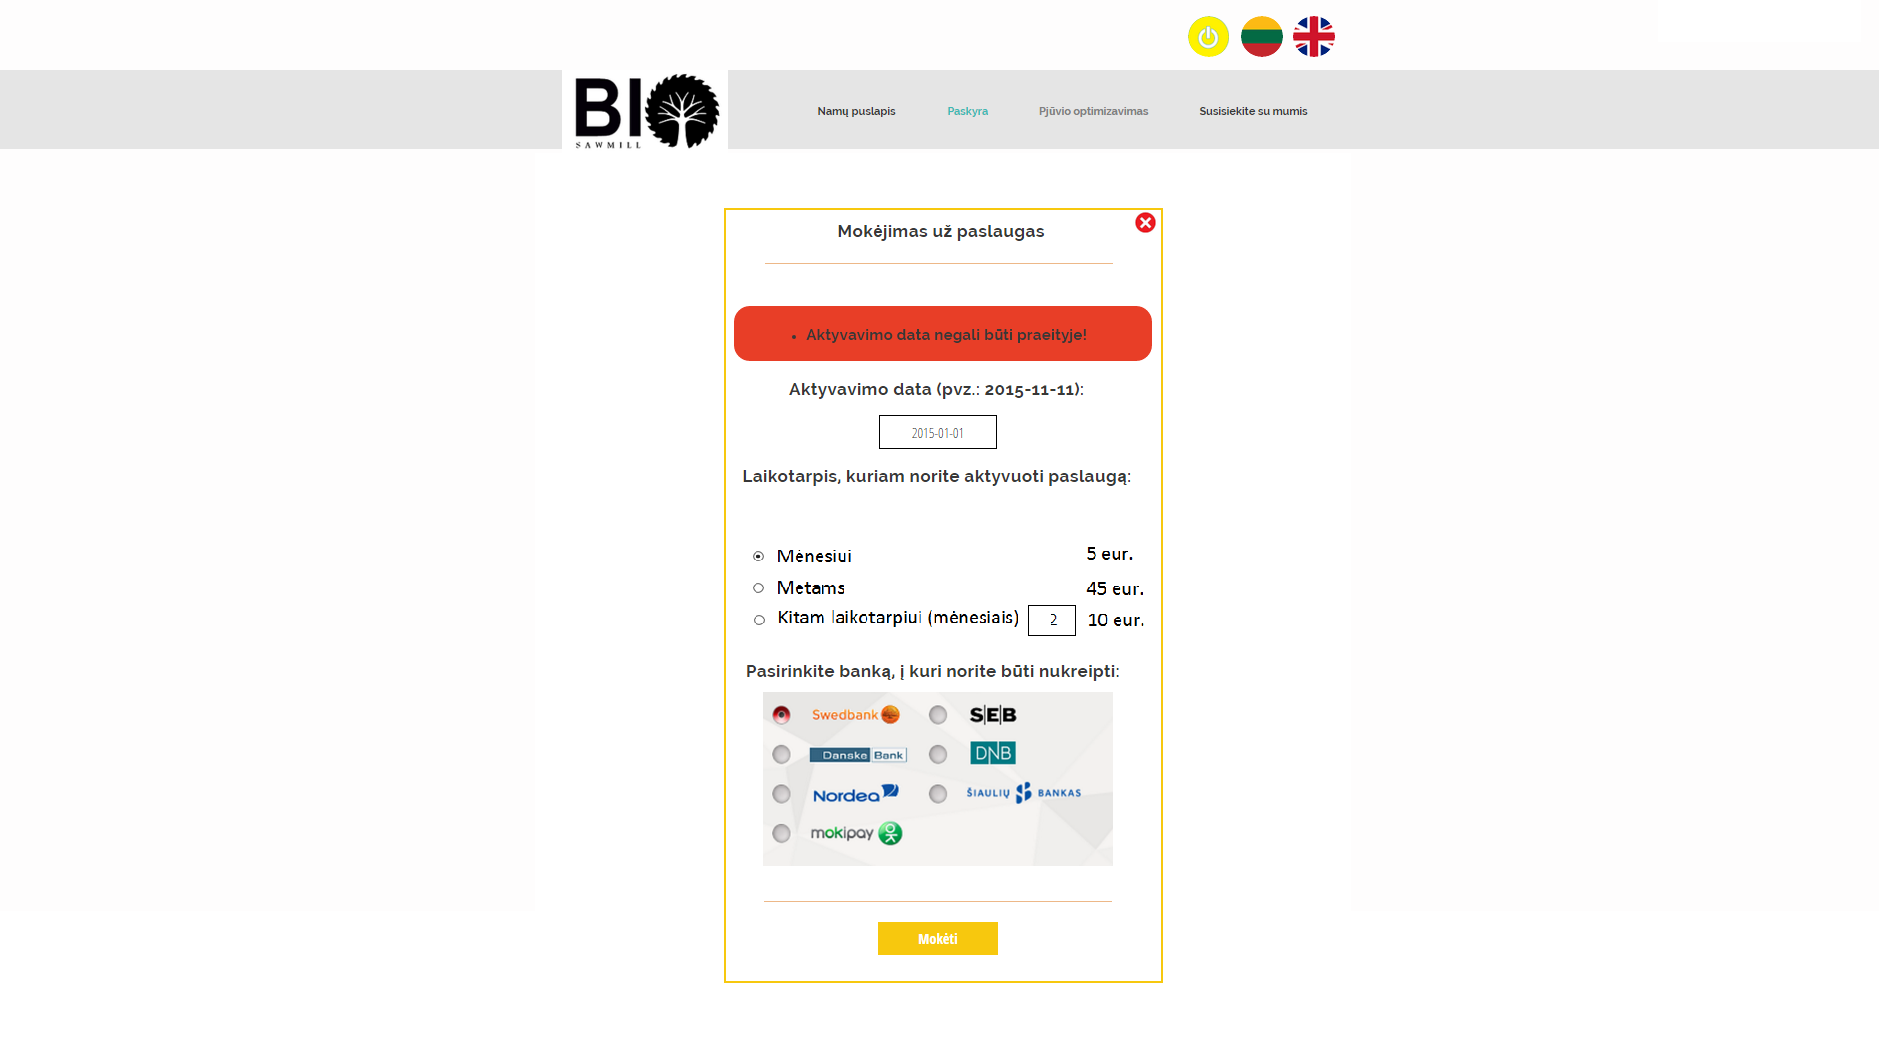
\includegraphics[scale=0.5]{interfeisai/paskyrosPuslapisVartotojasMokejimasSuKlaida}

\subsection{Vartotojo paskyros puslapis - administratorius}
\hspace{-2cm}
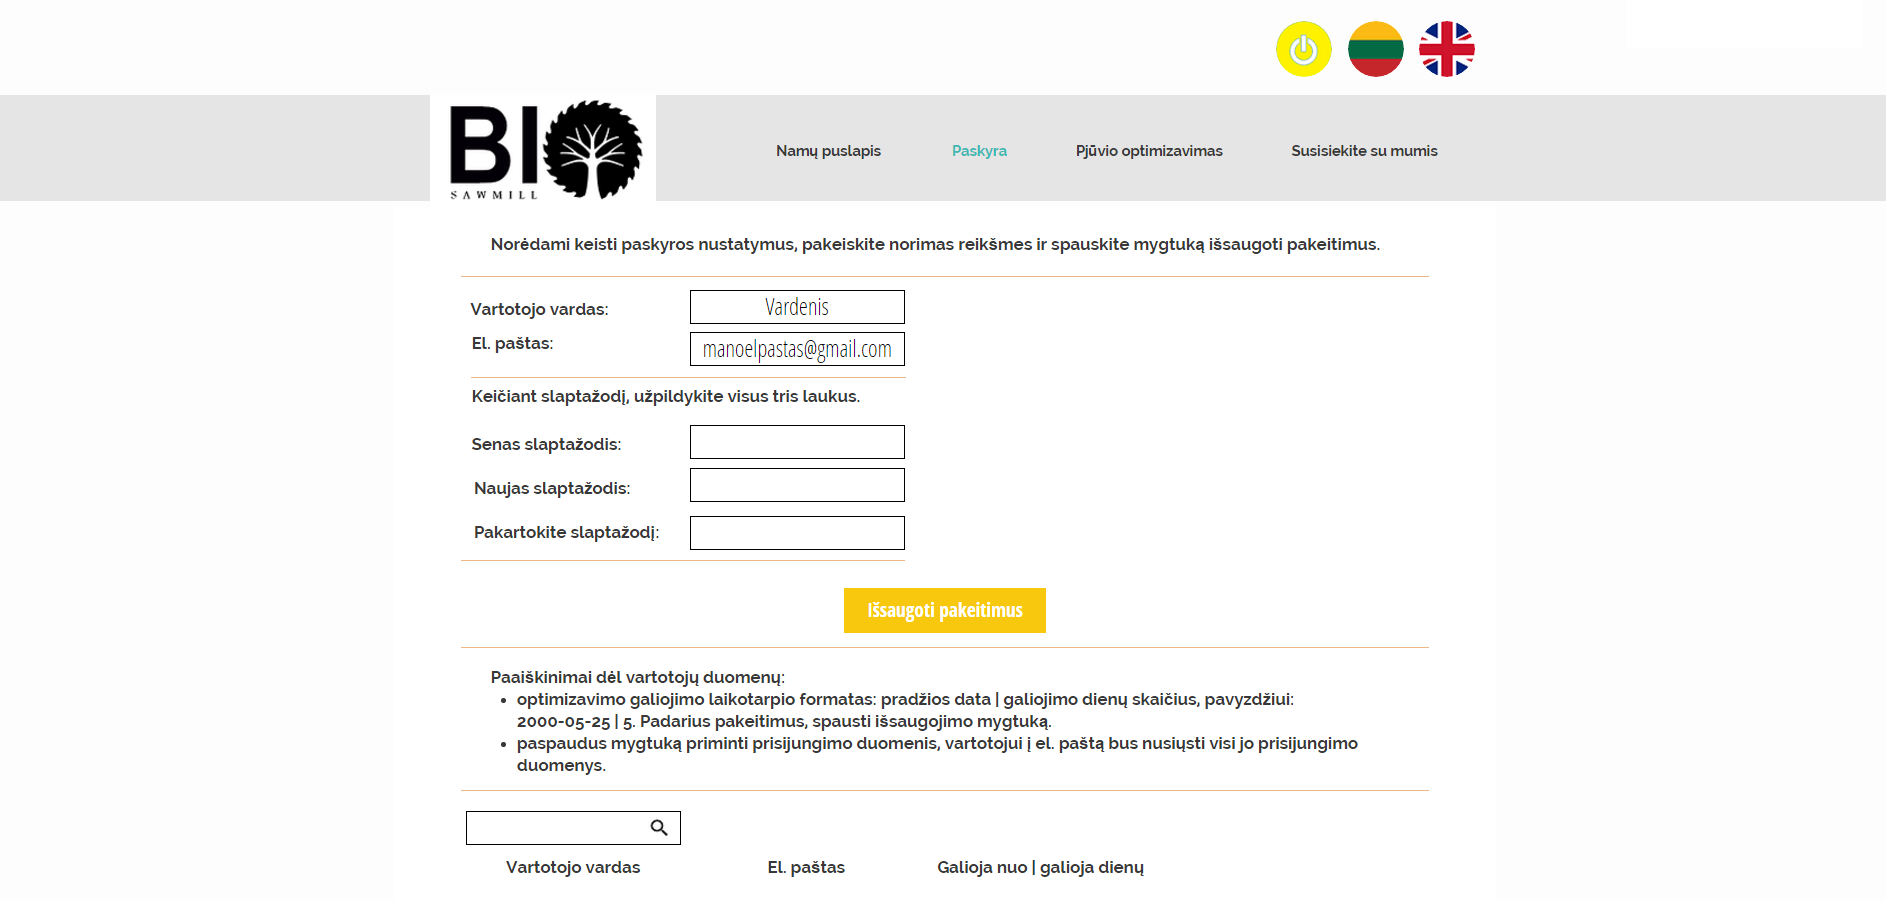
\includegraphics[scale=0.5]{interfeisai/paskyrosPuslapisAdministratorius}

\subsection{Vartotojo paskyros puslapis - administratorius (su klaida)}
\hspace{-2cm}
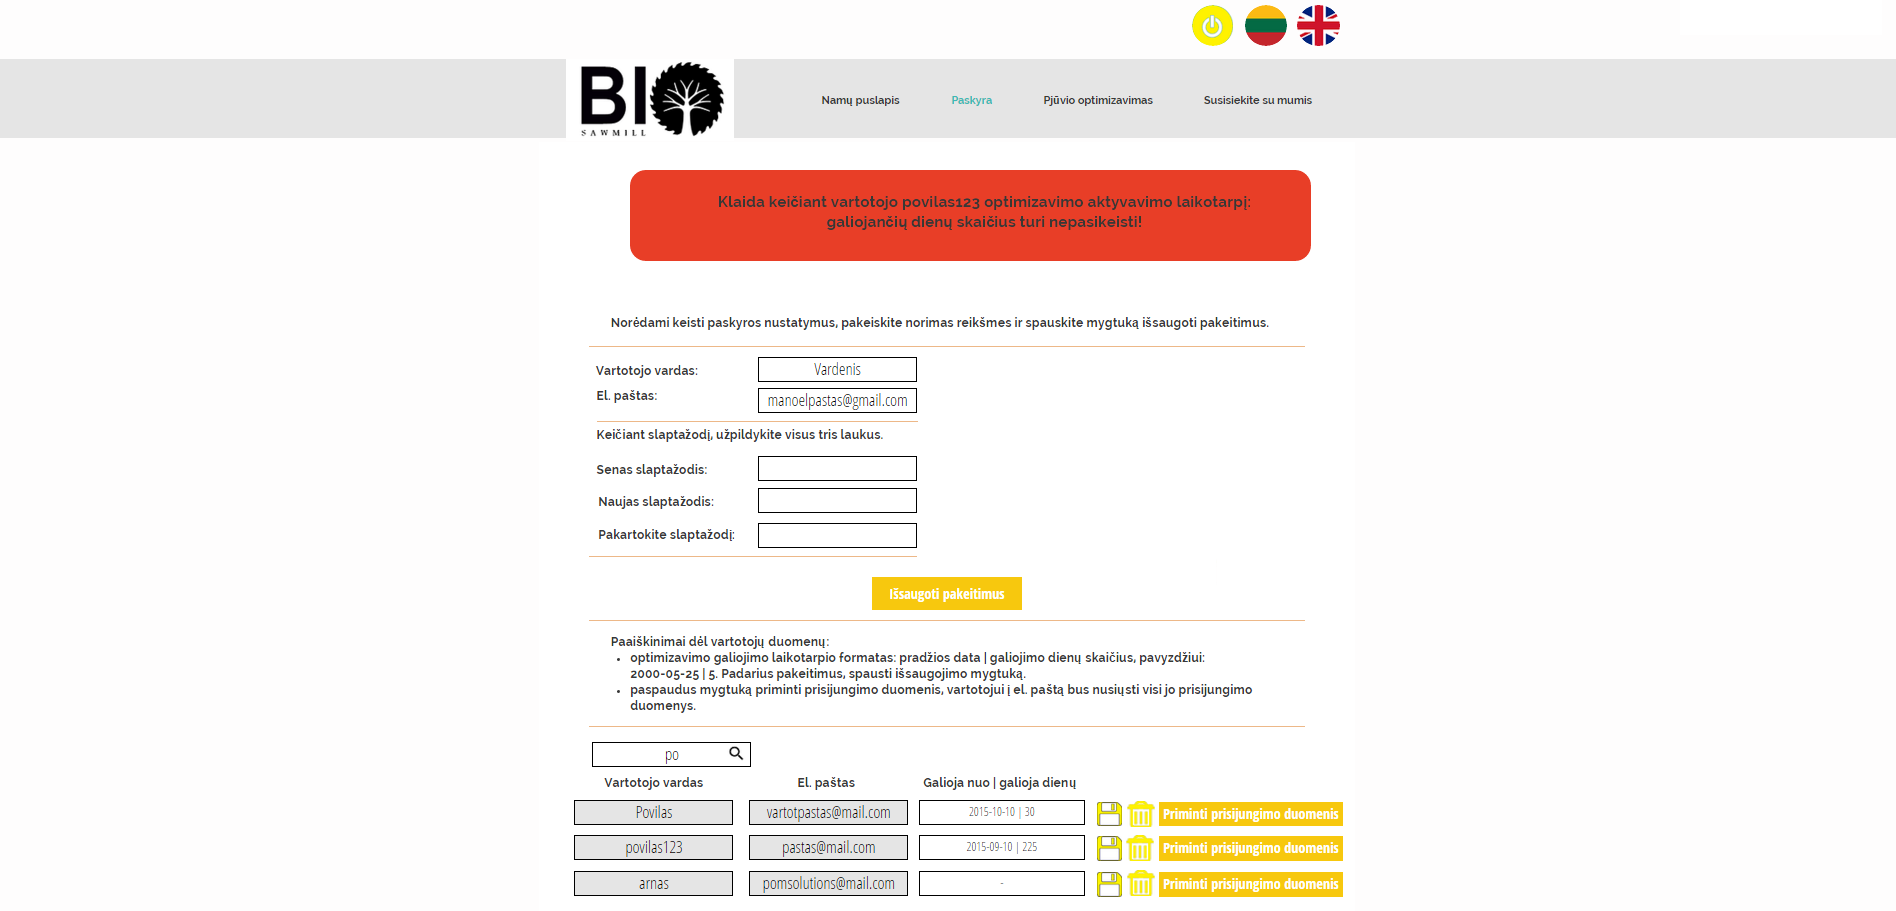
\includegraphics[scale=0.5]{interfeisai/paskyrosPuslapisAdministratoriusSuKlaida}

\subsection{Optimizavimo puslapis - neprisijungus}
\hspace{-2cm}
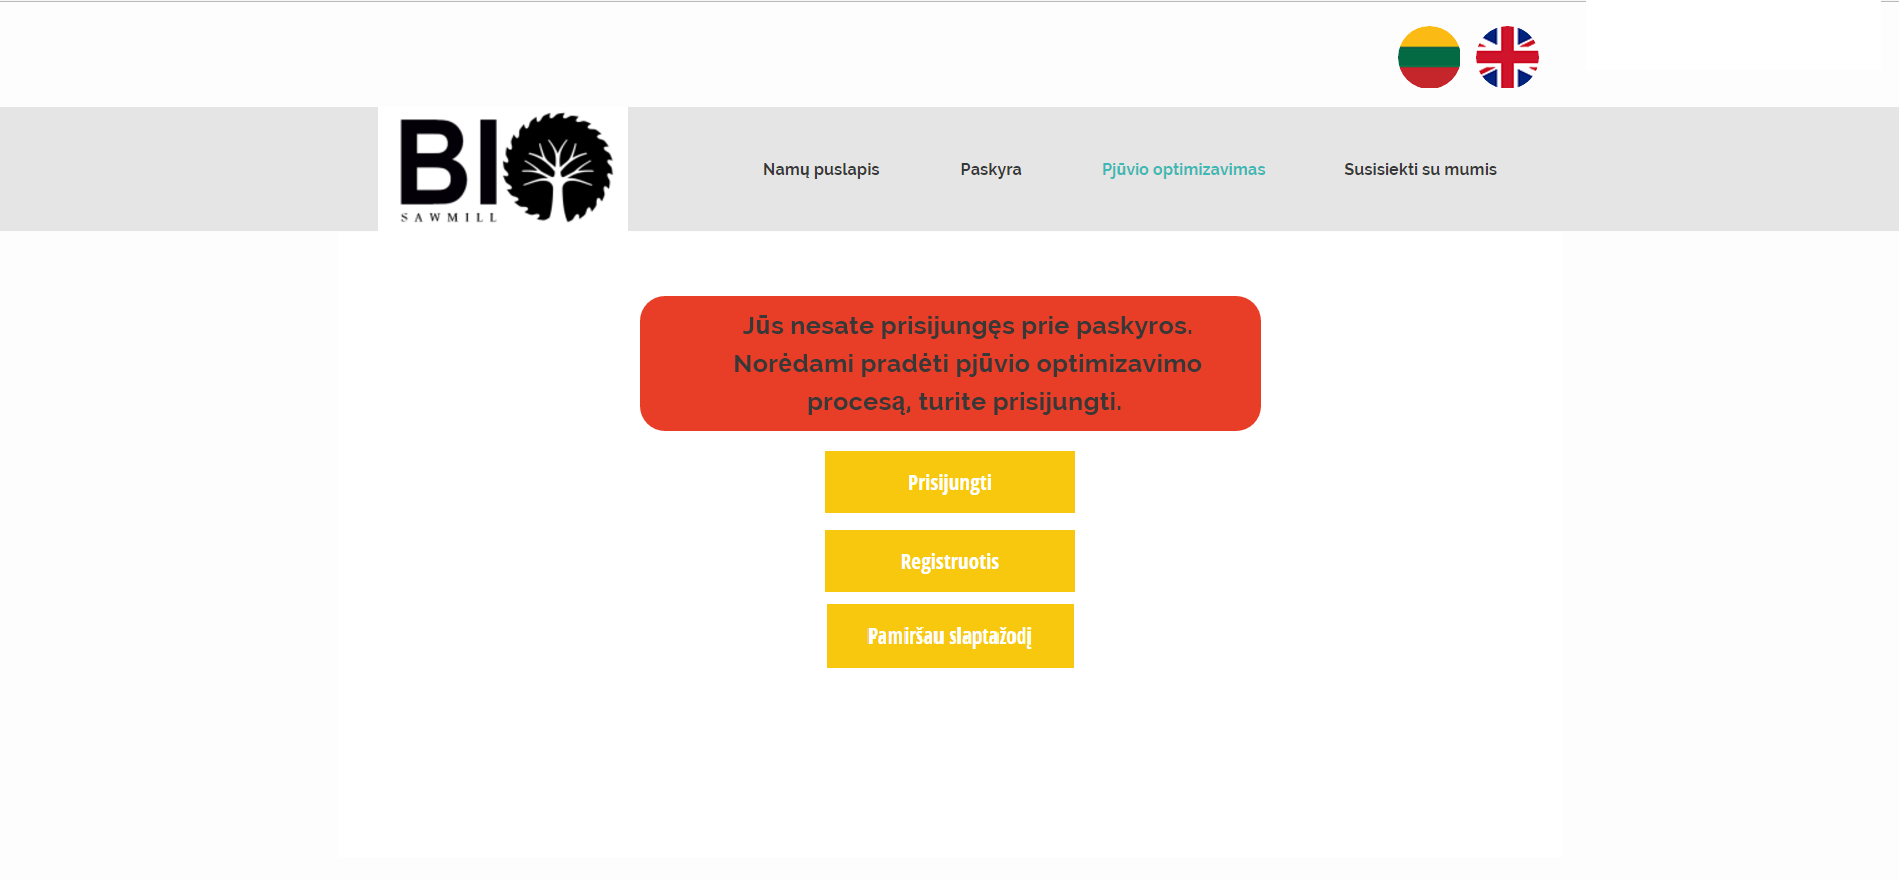
\includegraphics[scale=0.5]{interfeisai/optimizavimoPuslapisNeprisijungus}

\subsection{Optimizavimo puslapis - prisijungus}
\hspace{-2cm}
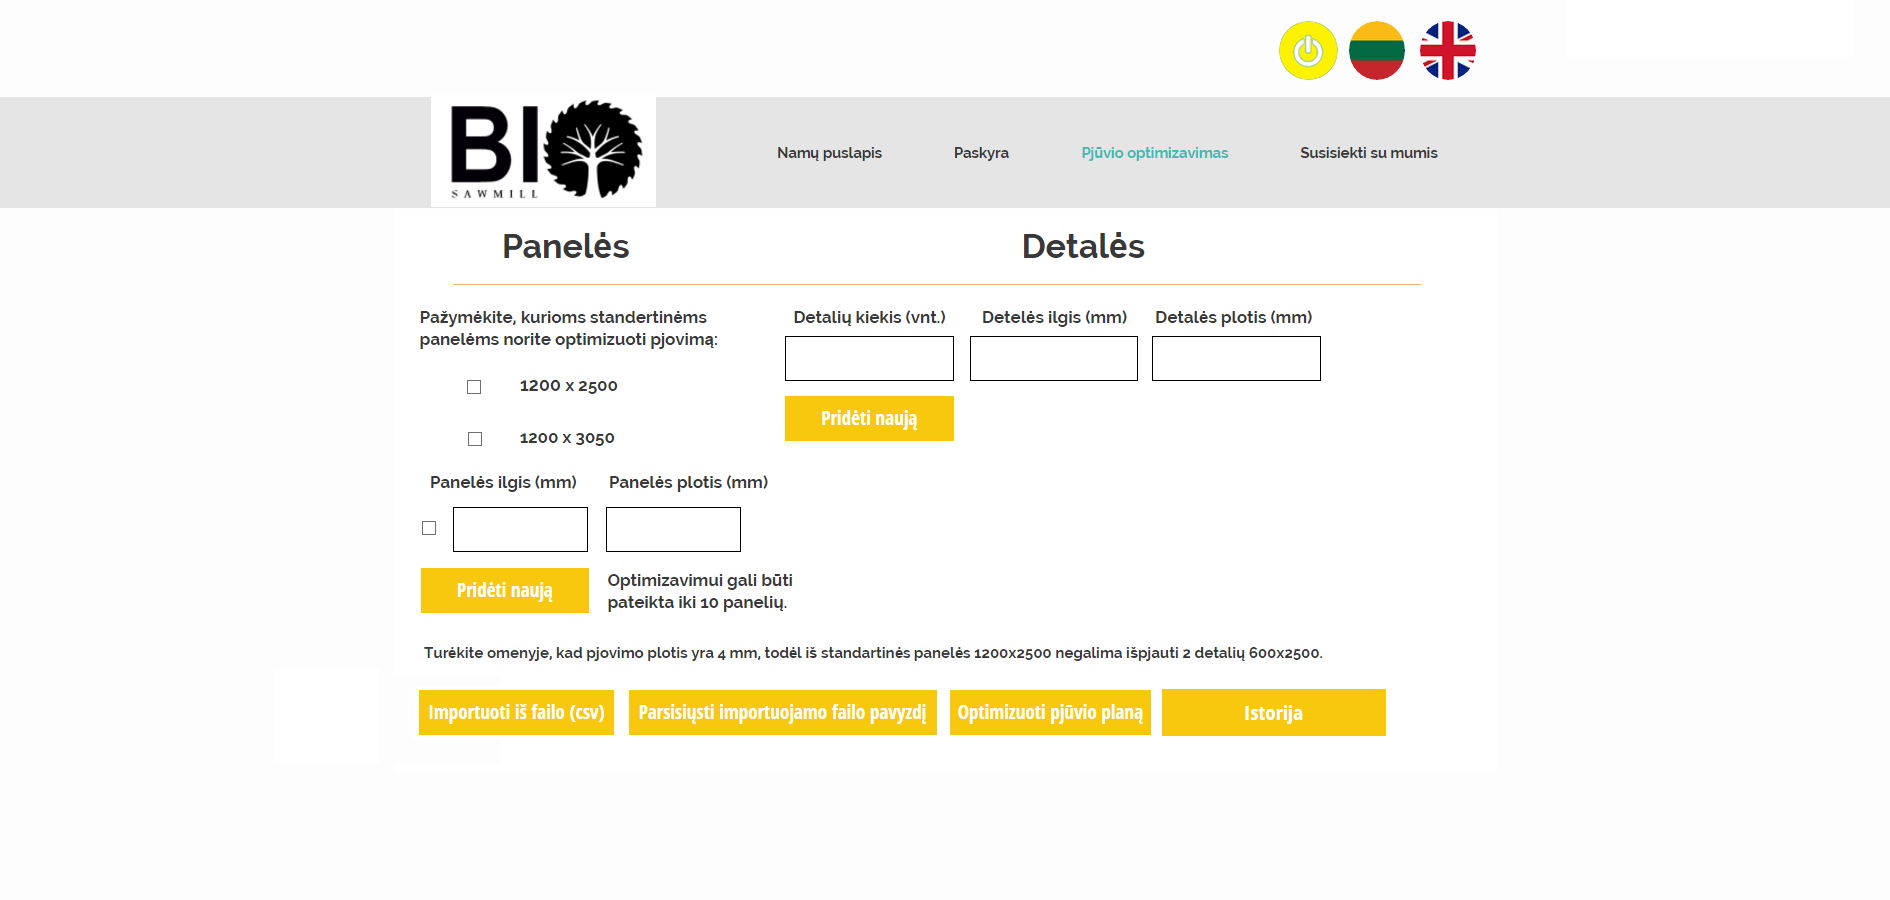
\includegraphics[scale=0.5]{interfeisai/optimizavimoPuslapisPrisijungus}

\subsection{Optimizavimo puslapis - prisijungus (su klaida)}
\hspace{-2cm}
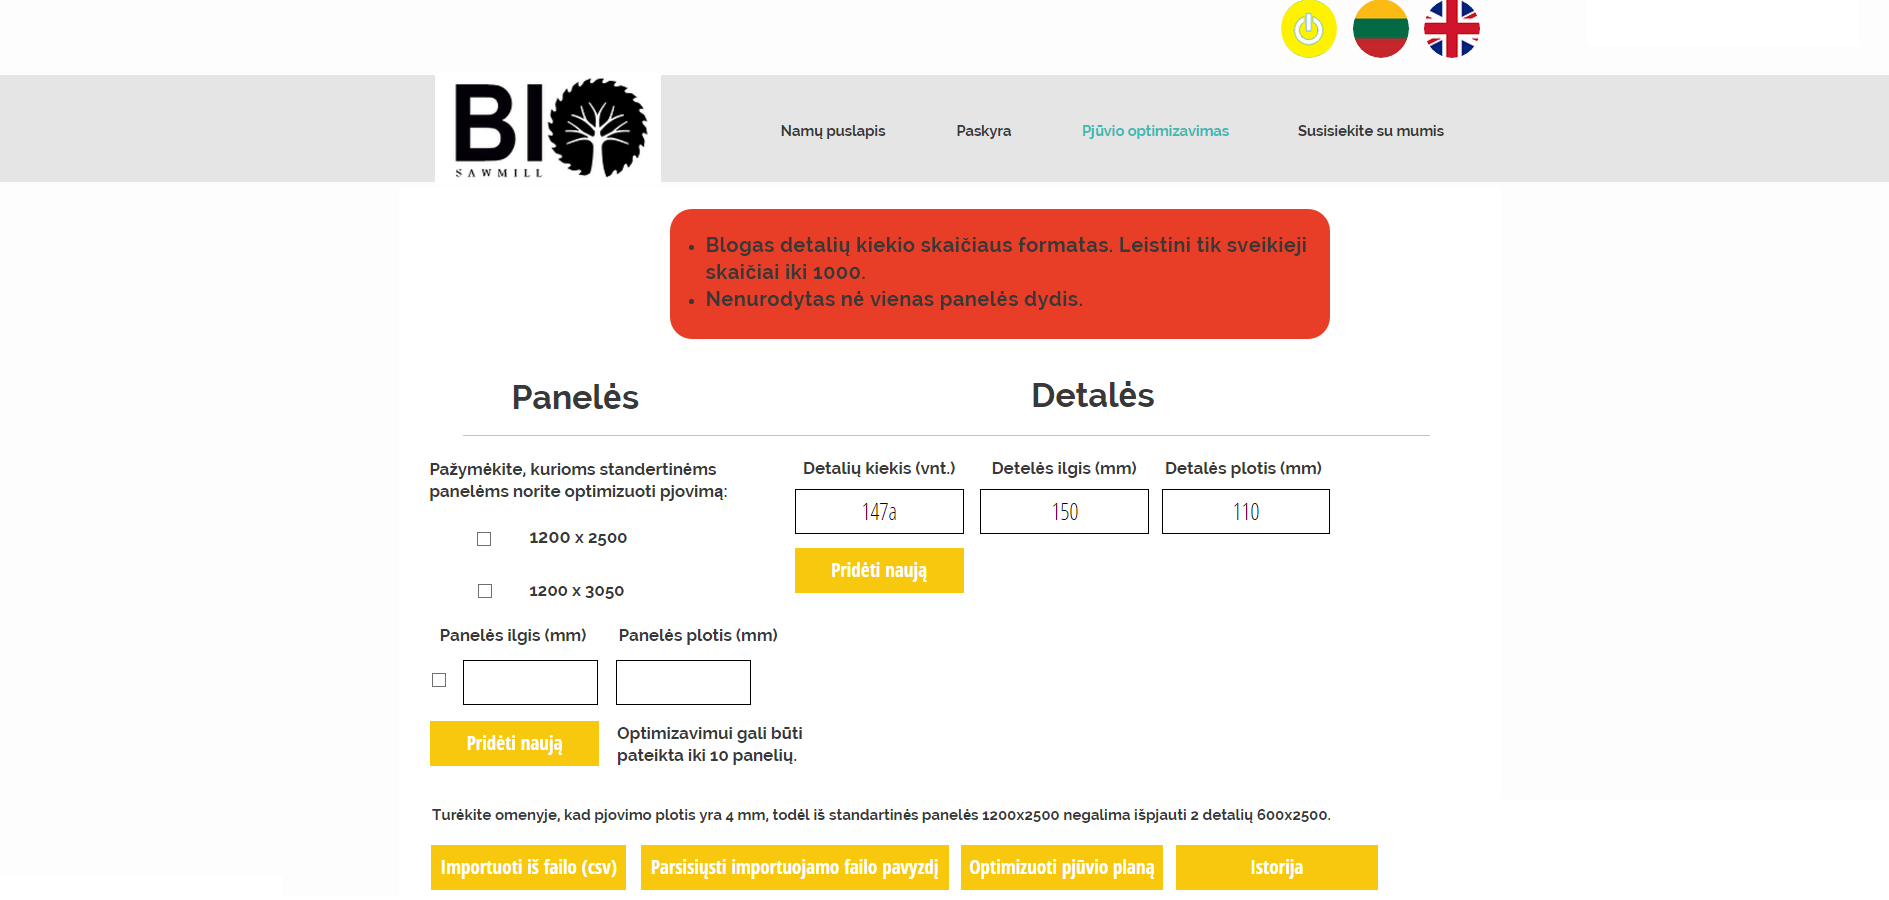
\includegraphics[scale=0.5]{interfeisai/optimizavimoPuslapisPrisijungusSuKlaida}

\subsection{Optimizavimo puslapis - po optimizavimo proceso}
\hspace{-2cm}
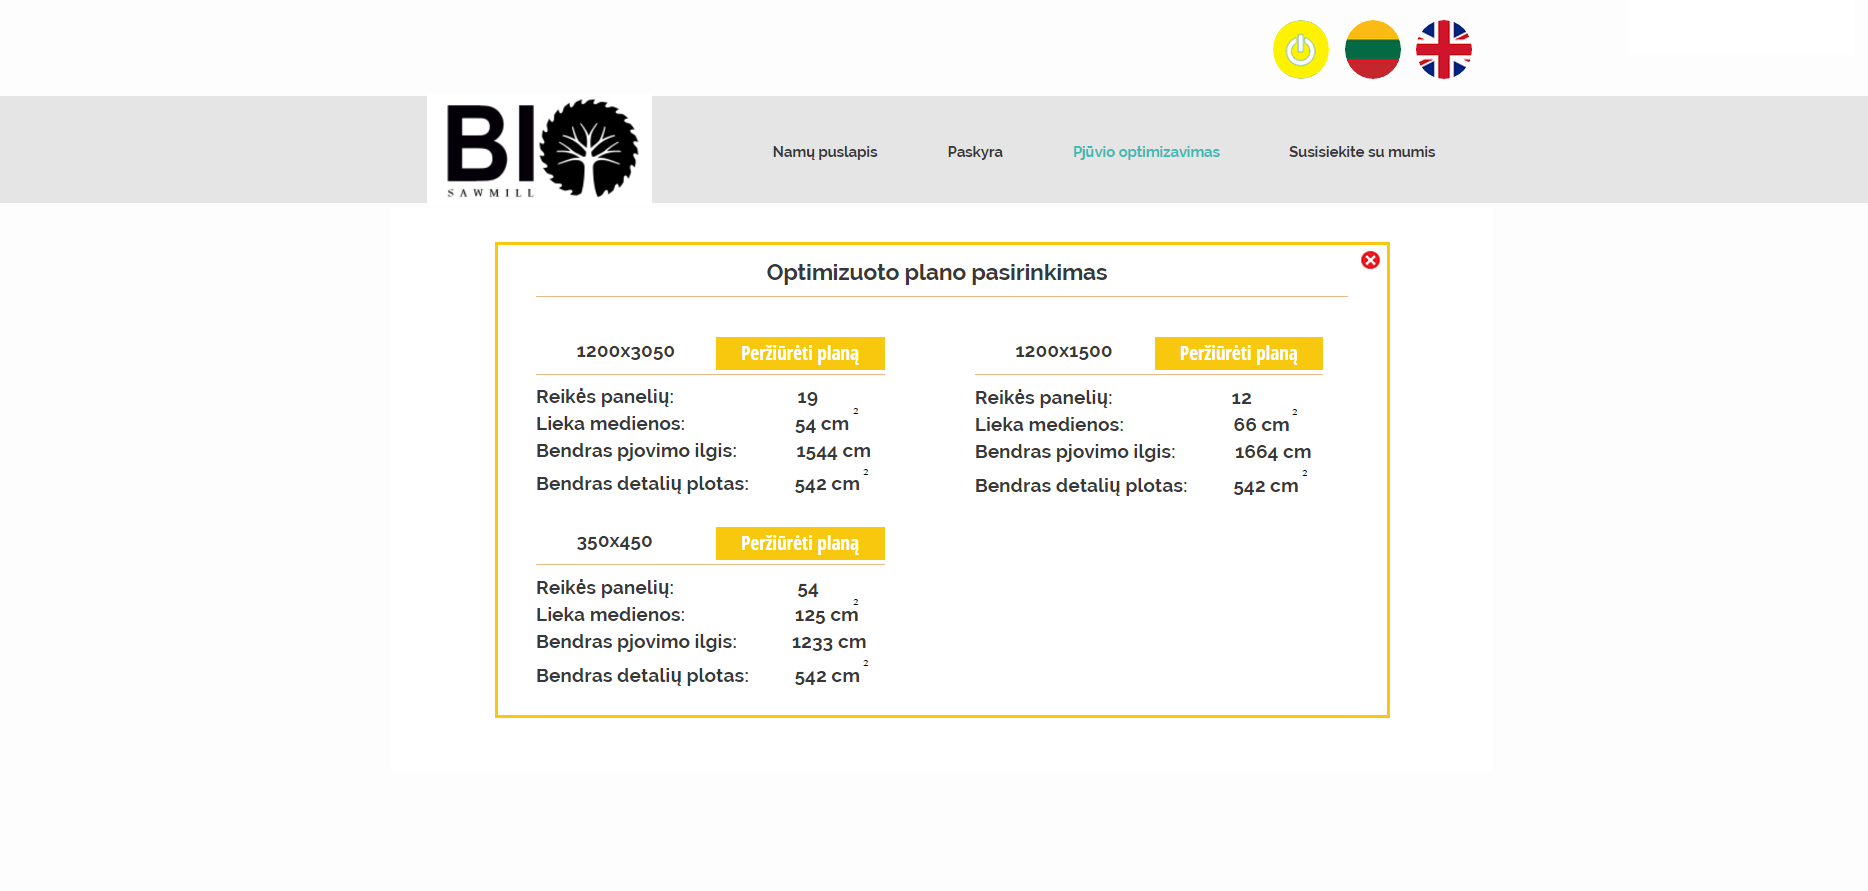
\includegraphics[scale=0.5]{interfeisai/optimizavimoPuslapisOptimizuotiPlanai}

\subsection{Optimizavimo puslapis - po optimizavimo, pasirinkus vieno iš planų peržiūrą}
\hspace{-2cm}
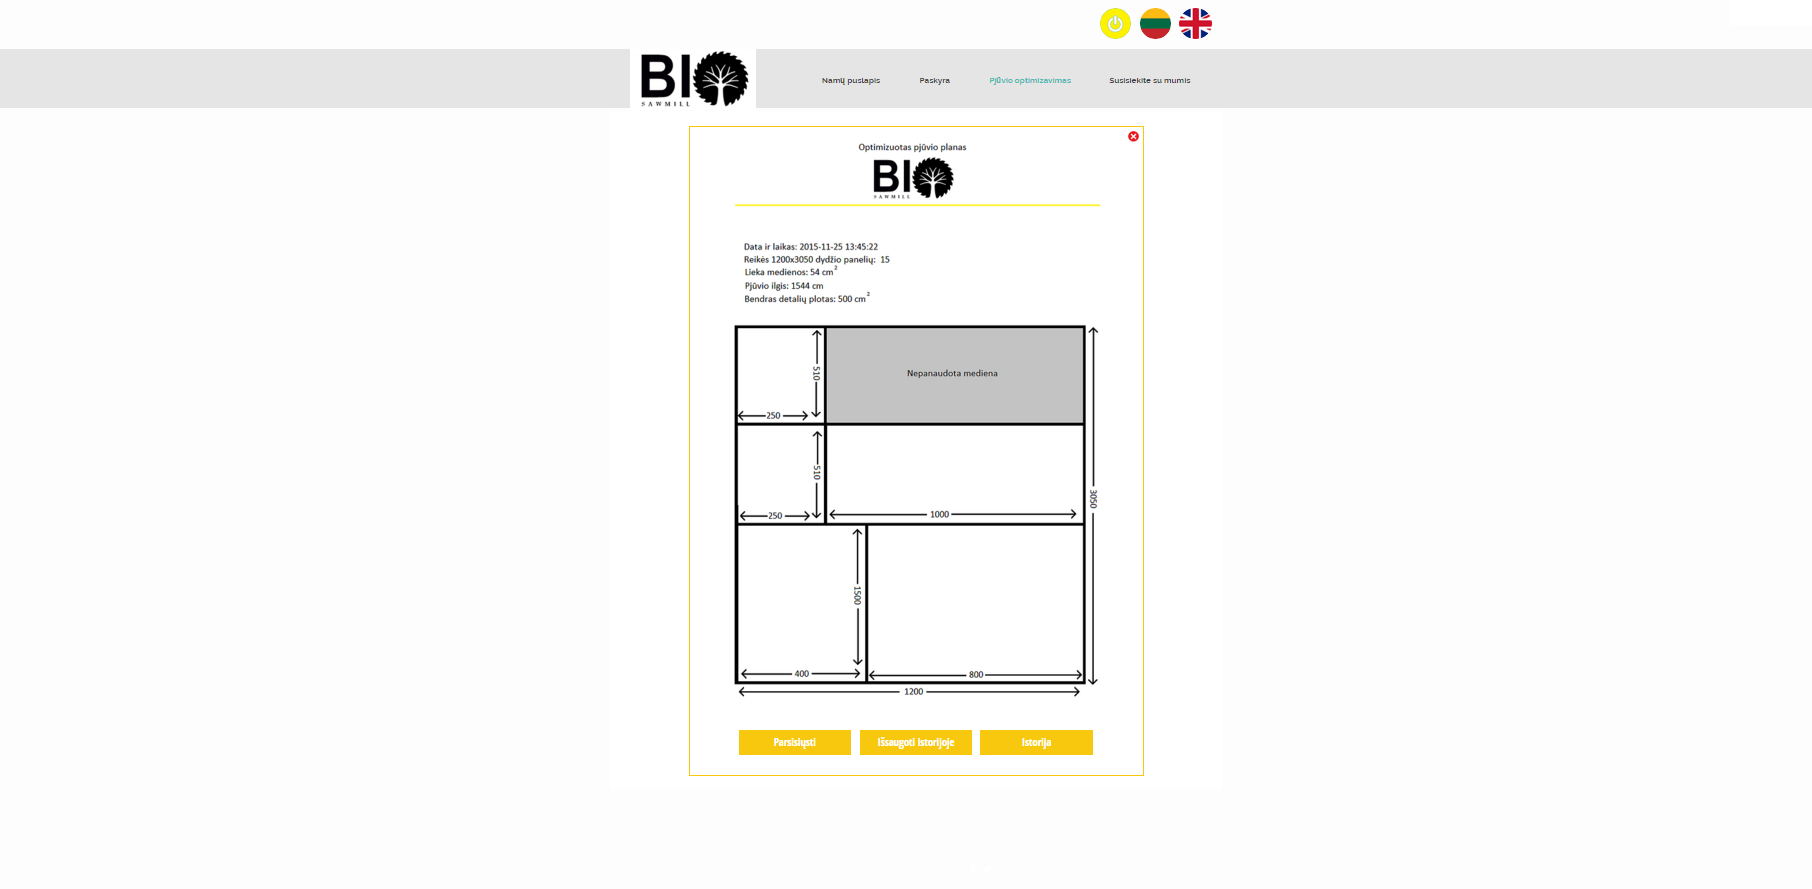
\includegraphics[scale=0.5]{interfeisai/optimizavimoPuslapisPrisijungusPasirinktoPerziura}

\subsection{Optimizavimo puslapis - po optimizavimo, pasirinkus vieno iš planų peržiūrą (iš arčiau)}
\hspace{-2cm}
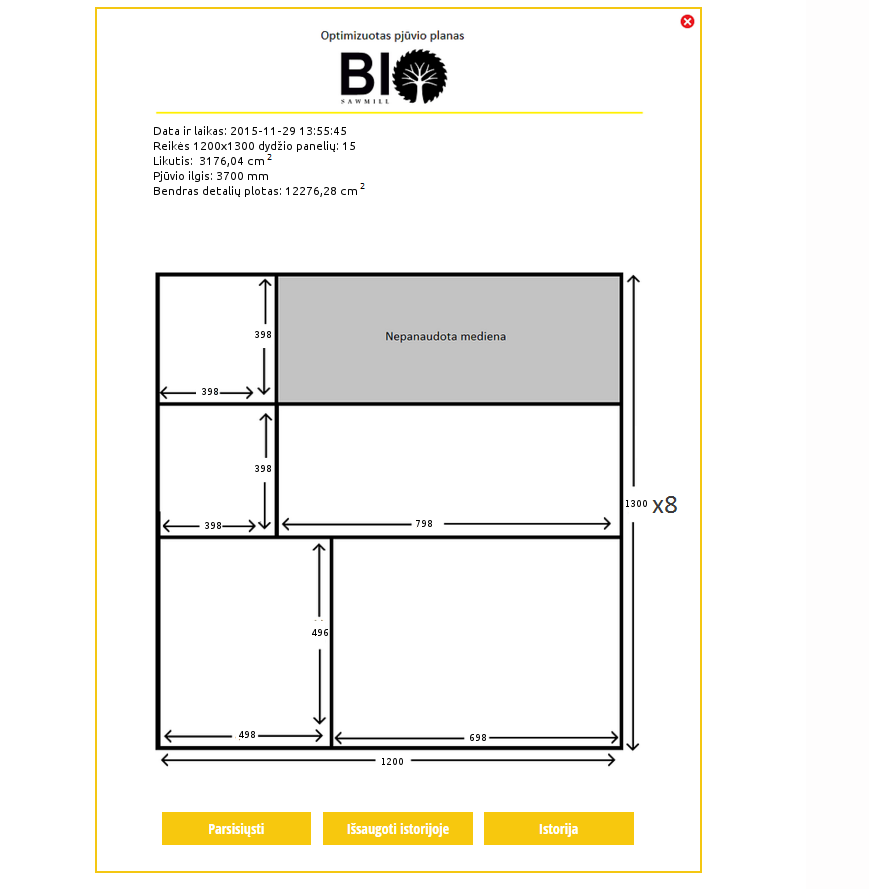
\includegraphics[scale=1.2]{interfeisai/optimizavimoPuslapisPrisijungusPasirinktoPerziura2}

\subsection{Optimizavimo puslapis - pasirinkto plano išsaugojimas}
\hspace{-2cm}
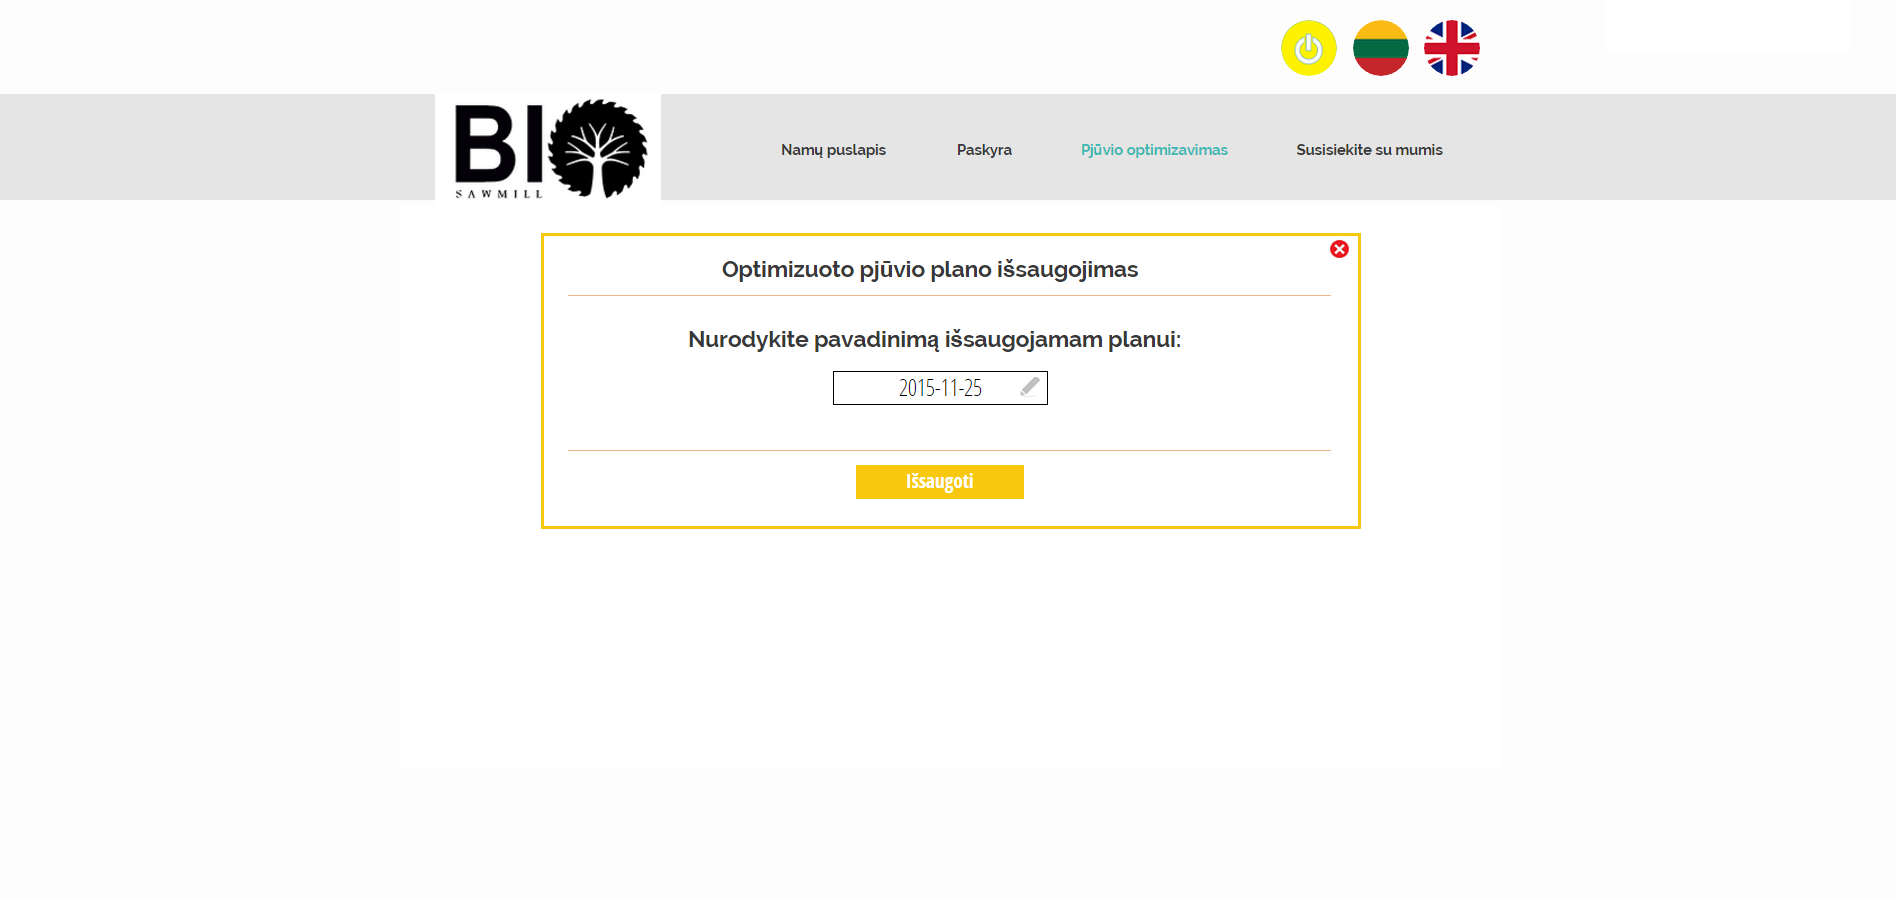
\includegraphics[scale=0.5]{interfeisai/optimizavimoPuslapisPrisijungusPasirinktoPlanoIsaugojimas}

\subsection{Optimizavimo puslapis - pasirinkto plano išsaugojimas (su klaida)}
\hspace{-2cm}
\includegraphics[scale=0.5]{interfeisai/optimizavimoPuslapisPrisijungusPasirinktoPlanoIsaugojimasSuKlaida}

\subsection{Optimizavimo puslapis - istorijos peržiūra}
\hspace{-2cm}
\includegraphics[scale=0.5]{interfeisai/optimizavimoPuslapisPrisijungusIstorija}

\subsection{Optimizavimo puslapis - istorijos redagavimas (su klaida)}
\hspace{-2cm}
\includegraphics[scale=0.5]{interfeisai/optimizavimoPuslapisPrisijungusIstorijaSuKlaida}

\subsection{Optimizavimo puslapis - išsaugoto plano istorijoje peržiūra (iš arčiau)}
\hspace{-2cm}
\includegraphics[scale=1.2]{interfeisai/optimizavimoPuslapisPrisijungusIsaugotasPlanas}

\subsection{Susisiekimo su mumis puslapis}
\hspace{-2cm}
\includegraphics[scale=0.5]{interfeisai/susisiekimas}

\subsection{Susisiekimo su mumis puslapis (su klaida)}
\hspace{-2cm}
\includegraphics[scale=0.5]{interfeisai/susisiekimasSuKlaida}

\end{comment}
% ---------------------------------- ATKOMENTUOTA ------------------------------

\section{Klasių diagrama}


\section{Reikalavimų atsekamumų lentelė}

\end{document}
